\RequirePackage{xcolor}     % color extensions
\documentclass[fleqn]{fcup-thesis}
\usepackage{mysty}

\usepackage[english]{babel}
\usepackage{lipsum}  % dummy text
\usepackage[utf8]{inputenc}
\usepackage[T1]{fontenc}
\usepackage{lmodern}
\usepackage{amsmath,amssymb,bm}
\usepackage{mathtools}
\usepackage{graphicx}
\usepackage[separate-uncertainty=true]{siunitx}    % SI units
\usepackage[version=3]{mhchem}  				   % checmial formular
\usepackage{wasysym}
\usepackage[final]{microtype}
\usepackage[hang,multiple]{footmisc}
\let\newfloat\relax
\usepackage{float}
\usepackage{placeins}
\usepackage{xkvltxp}
\usepackage{fixme} 						           % add fixme to draft documents
\usepackage{color}
\usepackage{rotate}
\usepackage{rotating}
\usepackage{listings}
\usepackage{booktabs}   				     	   % improved quality tables
\usepackage{threeparttable}
\usepackage{threeparttablex}     			       % Lets threeparttable work with longtable
\usepackage{longtable}
\usepackage{pdflscape}
\usepackage{datatool}			% Loading in databases into table

\usepackage{caption}
\captionsetup{labelfont=bf}
\captionsetup[table]{justification=justified,singlelinecheck=false,}

\definecolor{flatblue}{RGB}{41, 128, 185}
\definecolor{flatgrey}{RGB}{52, 73, 94}
\definecolor{flatgreen}{RGB}{44, 201, 144}
\definecolor{flatpurple}{RGB}{142, 68, 173}
\definecolor{flatorange}{RGB}{211, 84, 0}
\definecolor{flatred}{RGB}{207, 0, 15}
\usepackage{soul}  % highlight text with \hl{}, strikethrough with \st{}
\sethlcolor{flatgreen}
\setstcolor{flatred}
\usepackage{epigraph} %for quotes
\setlength\epigraphrule{0pt}

%% TODO NOTES
\usepackage{xargs}                      % Use more than one optional parameter in a new commands
\usepackage[colorinlistoftodos,prependcaption,textsize=tiny]{todonotes}
\newcommandx{\change}[2][1=]{\todo[linecolor=flatblue,backgroundcolor=flatblue!25,bordercolor=flatblue,#1]{#2}}
\newcommandx{\reference}[2][1=]{\todo[linecolor=flatgreen,backgroundcolor=flatgreen!25,bordercolor=flatgreen,#1]{#2}}
\newcommandx{\unfinished}[2][1=]{\todo[linecolor=flatorange,backgroundcolor=flatorange!25,bordercolor=flatorange,#1]{#2}}
\newcommandx{\improvement}[2][1=]{\todo[linecolor=flatpurple,backgroundcolor=flatpurple!25,bordercolor=flatpurple,#1]{#2}}
\newcommand{\red}{\color{red}}

%%%%%%%%%%% Literature %%%%%%%%%%%%%%%
% When in doubt visit this page:
% http://adsabs.harvard.edu/abs_doc/aas_macros.html
\usepackage[authoryear]{natbib}
\def\aap{A\&A}
\def\aapr{Astronomy and Astrophysics Reviews}
\def\eprint{e-prints}
\def\apj{ApJ}
\def\apjs{ApJS}
\def\apjl{ApJL}
\def\mnras{MNRAS}
\def\aj{AJ}
\def\nat{Nature}
\def\aaps{A\&A Supp.}
\def\pasp{Publications of the ASP}
\def\prd{Phys. Rev. D}
\def\prl{Phys. Rev. Lett.}
\def\araa{ARA\&A}
\def\actaa{Acta Astronomica}
\def\procspie{Proceedings of the SPIE}
\def\pasj{PASJ}
\def\icarus{Icarus}
\def\pasa{Publications of the Astron. Soc. of Australia}


\usepackage{fix-cm} % Allows increasing the f
\usepackage[colorlinks,
linkcolor=flatorange,
citecolor=flatblue,
urlcolor=flatpurple]{hyperref}

\usepackage[Lenny]{fncychap}

\usepackage[format=hang]{caption}  % Make captions indent to end of Figure X:
%%%%%%%%%%%%% new commands %%%%%%%%%%%%%%%
\newcommand{\cref}[1]{Chapter~\ref{#1}}
\newcommand{\sref}[1]{Section~\ref{#1}}
\newcommand{\tref}[1]{\tablename~\ref{#1}}
\newcommand{\fref}[1]{\figurename~\ref{#1}}
\newcommand{\aref}[1]{Appendix~\ref{#1}}
\newcommand{\eref}[1]{Equation~\ref{#1}}
\renewcommand{\epsilon}{\varepsilon}
\renewcommand{\bf}{\textbf}
\newcommand{\nicebreak}{\newline\newline\noindent}
\newcommand{\code}[1]{\texttt{#1}}
\newcommand{\object}[1]{#1}
\newcommand{\Mjup}{M_\mathrm{Jup}}

%%%%%%%%%%%%%%%% Math %%%%%%%%%%%%%%%%%%%%
\newcommand{\F}{\mathcal{F}}
\newcommand{\tm}[1]{\textnormal{#1}}
\newcommand{\pd}[2]{\frac{\partial #1}{\partial #2}}
\newcommand{\dd}[2]{\frac{\mathrm{d} #1}{\mathrm{d} #2}}

%%%%%%%%%%%%% Layout %%%%%%%%%%%%%%%%%%%%%
\setcounter{secnumdepth}{3}
\setcounter{tocdepth}{3}

%% A&A stuff
\DeclareRobustCommand{\ion}[2]{\textup{#1\,\textsc{\lowercase{#2}}}}
\newcommand*\element[1][]{%
	\def\aa@element@tr{#1}%
	\aa@element
}

%% SI units
\DeclareSIUnit\photons{photons}


%% word shortcuts
\newcommand{\thar}{Th-Ar}  
\newcommand{\nir}{nIR}
\newcommand{\logg}{logg}
\newcommand{\feh}{$\textrm{[Fe/H]}$}
\newcommand{\teff}{T_\mathrm{eff}}






%% *** Change this example to appropriate values. ***
\degree{Doctor of Philosophy}
\department{Departamento de F\'isica e Astronomia}
\gradyear{2018}
\author{Jason James Neal}
\title{Towards the nIR detection of exoplanets}


%% Make each page fill up the entire page.
\flushbottom

\listfiles

%%%%%%%%%%%%      MAIN  DOCUMENT      %%%%%%%%%%%%
% \includeonly{introduction}

\begin{document}
	
	%% This sets the page style and numbering for preliminary sections.
	\begin{preliminary}
		
		%% This generates the title page from the information given above.
		\maketitle
		\cleardoublepage
		
		
		\begin{dedication}
			\centering \huge \itshape
			To Jessica, Timothy, Amelia\\For always supporting me
		\end{dedication}
		
		
		\begin{acknowledgements}
			
			Gillian - proofreading
			
			Supervisors for guiding me
			
			\vspace{7mm}
			
			
		\end{acknowledgements}
		
		
		
		\begin{abstract}
			
			Thesis abstract
		\end{abstract}
		
		\begin{abstract-pt}
			
			Thesis abstract in Portuguese
		\end{abstract-pt}
		
		
		 %%% remove in final version
        \todototoc
		\listoftodos
        
		\tableofcontents
		\addcontentsline{toc}{chapter}{\listtablename}
		\listoftables
		\addcontentsline{toc}{chapter}{\listfigurename}
		\listoffigures
        
       
        
        
		\begin{abbreviations}		
			\begin{longtable}{ll}
				
				Carmenes & Calar Alto high-Resolution search for M dwarfs with Exoearths with Near-infrared and optical \'Echelle Spectrographs \\
				CFHT & Canada France Hawaii Telescope \\
				CRIRES & CRyogenic high-resolution InfraRed \'Echelle Spectrograph \\
				E-ELT & European-Extremely Large Telescope \\
				ESO & European Southern Observatory \\
				ESPRESSO & \'Echelle SPectrograph for Rocky Exoplanet and Stable Spectroscopic Observations\\
				FIRST & Florida InfraRed Silicon immersion grating spectromeTer \\
				HET & Hobby-Eberly Telescope \\
				HPF & Habitable Planet Finder \\
				IR & Infrared\\
				JWST & James Web Space Telescope \\
				MIR & Mid-Infrared \\
				MIRI & Mid-Infrared Instrument\\
				NASA & National Aeronautics and Space Administration \\
				NIR & Near-Infrared \\
				SPIRou & SpectroPolarim\`etre Infra-Rouge\\
				TMT & Thirty Meter Telescope\\
				TNG & Telescopio Nazionale Galileo \\
				VISIR &  VLT spectrometer and imager for the mid-infrared \\
				VLT & Very large Telescope \\
				
			\end{longtable}		
		\end{abbreviations}
		
		\begin{constants}
			\begin{longtable}{lr@{${}={}$}l}
				 % The \SI{}{} command is provided by the siunitx package, see its documentation for instructions on how to use it
				 
				 Speed of Light & $c_{0}$ & \SI{2.99792458e8}{\meter\per\second} (exact)\\
				 Astronomocal Unit & AU & 150 million km\\
				 %Constant Name & $Symbol$ & $Constant Value$ with units\\	
			\end{longtable}
		\end{constants}
		
		\begin{symbols}
				\begin{longtable}{lll}
					
					$a$ & distance & \si{\metre} \\
					$P$ & power & \si{\watt} (\si{\joule\per\second}) \\
					%Symbol & Name & Unit \\
					
					\addlinespace % Gap to separate the Roman symbols from the Greek
					\\
					$\lambda$ & wavelength & \si{\nano\metre} \\
                    \(S_{tel}\) & telescope collecting area & \si{\centi\metre\squared} \\
                    \(N_{e^{-}}\) & number of photoelectrons & \\
                    \(P_{avg}\) & average monochromatic stellar brightness & \si{\photons\per\second\per\centi\metre\squared\per\centi\metre}\\
                    \(T_{exp}\) & exposure time  & \si{\second} \\ 
          
                    \(\Lambda\) & wavelength range & \si{\nano\metre} 
				\end{longtable}
		\end{symbols}
		
	\end{preliminary}
	
	
	%% *** Include chapter files here. ***
	%!TEX root = ../thesis.tex
\chapter{Introduction}\label{cha:introduction}


\section{Towards the characterization of exoplanets}

The field of exoplanetary science is rapidly accelerating with large scientific and instrumental investments undertaken, with the ultimate goal of detecting and characterizing an Earth-like planet, with the potential for life (as we know it).
Since the very first exoplanet detection\footnote{around a Sun-like star}~\citep{mayor_jupitermass_1995} the number of confirmed\footnote{Validated by more than one detection method} exoplanets has grown to over 3790 with almost another 3000 candidates awaiting confirmation\footnote{\href{https://exoplanets.nasa.gov/}{exoplanets.nasa.govt} as of October 2018}.
However, simply detecting the presence of exoplanets is not nearly enough to satisfy our quest for knowledge.
There is an exorbitant amount to be gained through the full characterization of these known exoplanets: density, composition, internal structure, atmosphere properties, and surface temperature.

When an Earth-twin planet is suspected (there have been several false claims already \textbf{~\citep[e.g.][]{mullally_kepler_2018} \textbf{more}\todo{other dead earth-like planets} other earth like planets shown to not be earth like or redacted papers}) a full characterization is required to confirm it's habitability \textbf{(ref)}.
For instance, knowing only the mass and radius can provide an average density but not the composition or the internal structure~\textbf{ref cite {a paper about composition degeneracy}}.
The presence of an exoplanet's atmosphere will also influence the average density but can provide detectable clues on the planet's composition.
Several techniques being explored to detect and characterize exoplanet atmospheres~\citep[e.g.][]{snellen_orbital_2010, martins_reflected_2016, piskorz_evidence_2016} \textbf{a transmission spectroscopy paper} with several recent advancements.

In this chapter the common exoplanet and atmospheric detection methods will be introduced, followed by some exoplanet property distributions and the motivation for the work performed in this thesis.\\


%!TEX root = ../../thesis.tex

\section{Exoplanet detection methods}
\label{sec:detection_methods}
There are several detection methods used to build up the picture of the current understanding of exoplanet candidates.
The different detection methods are often complementary, in that they are sensitive to different parameter spaces and are able to contribute different exoplanet properties, or detect different classes of exoplanet.
The simplest example is that planetary mass and radius are obtained from the radial velocity and transit methods separately.
Also the transit and radial velocity methods are both sensitive to large planets close to the star however, the direct imaging technique cannot see planets too close to the star, as the planets image is contaminated by the stellar image and speckles.

The exoplanet detection rates for different methods since 1995 are shown in \cref{fig:detection_year_method}.
The detection rates among different methods are not uniform, with the transit method having the majority of detections due to the use of the Kepler space telescope~\citep{borucki_finding_2008}.
The radial velocity method has a fairly consistent detection rate, while direct imaging and other methods have only made a small contribution to the total number of detections so far.
Details about the various main detection methods are provided in the following sections.

\begin{figure}
    \centering
    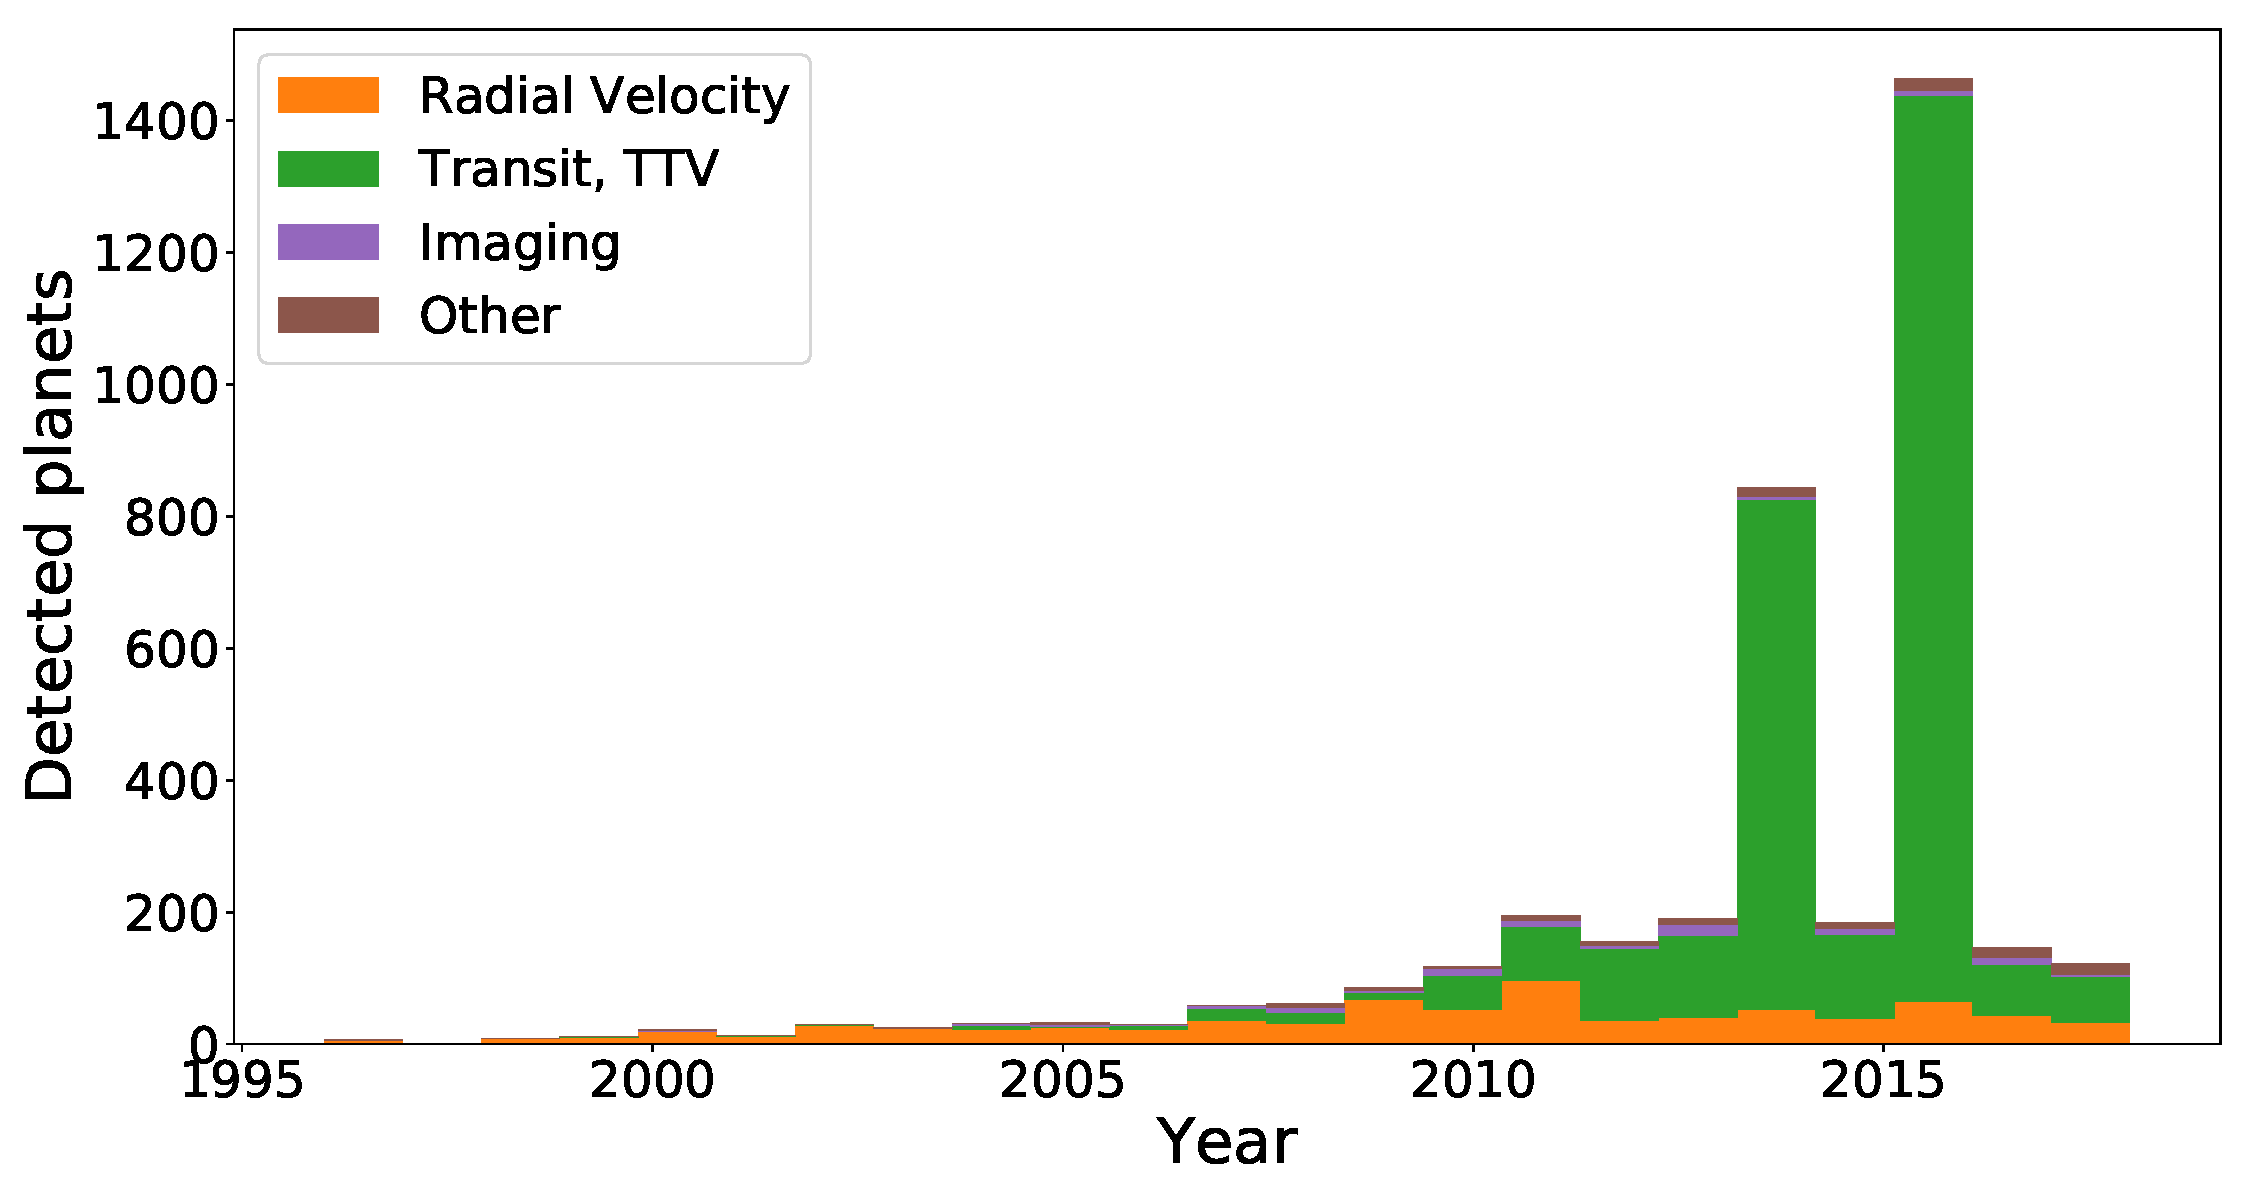
\includegraphics[width=0.7\linewidth]{./figures/introduction/exoplanetEU_year_method.pdf}
    \caption[Number of exoplanet detections per year separated by method.]{Number of exoplanet detections per year separated by method (data from \href{http://ww.exoplanet.eu}{exoplanet.eu} October 2018).}
    \label{fig:detection_year_method}
\end{figure}
\todo{Adjust figure so that can be seen in black and white, textures on bars?}
\subsection{Radial Velocimetry}
\label{subsec:radial_velocimetry}
This technique measures the radial velocity\footnote{Velocity projected along line of sight.} (RV) of the star by analysing the relative Doppler shift of its spectral lines due to the gravitational interaction with a companion.
As the star and companion orbit around their common centre of mass (barycentre) the spectrum of the star periodically oscillates, with the orbital period of the planet, due to the change in relative motion to the observer as depicted in \cref{fig:rvdiagram-mayor} (left).

\begin{figure}
    \centering
    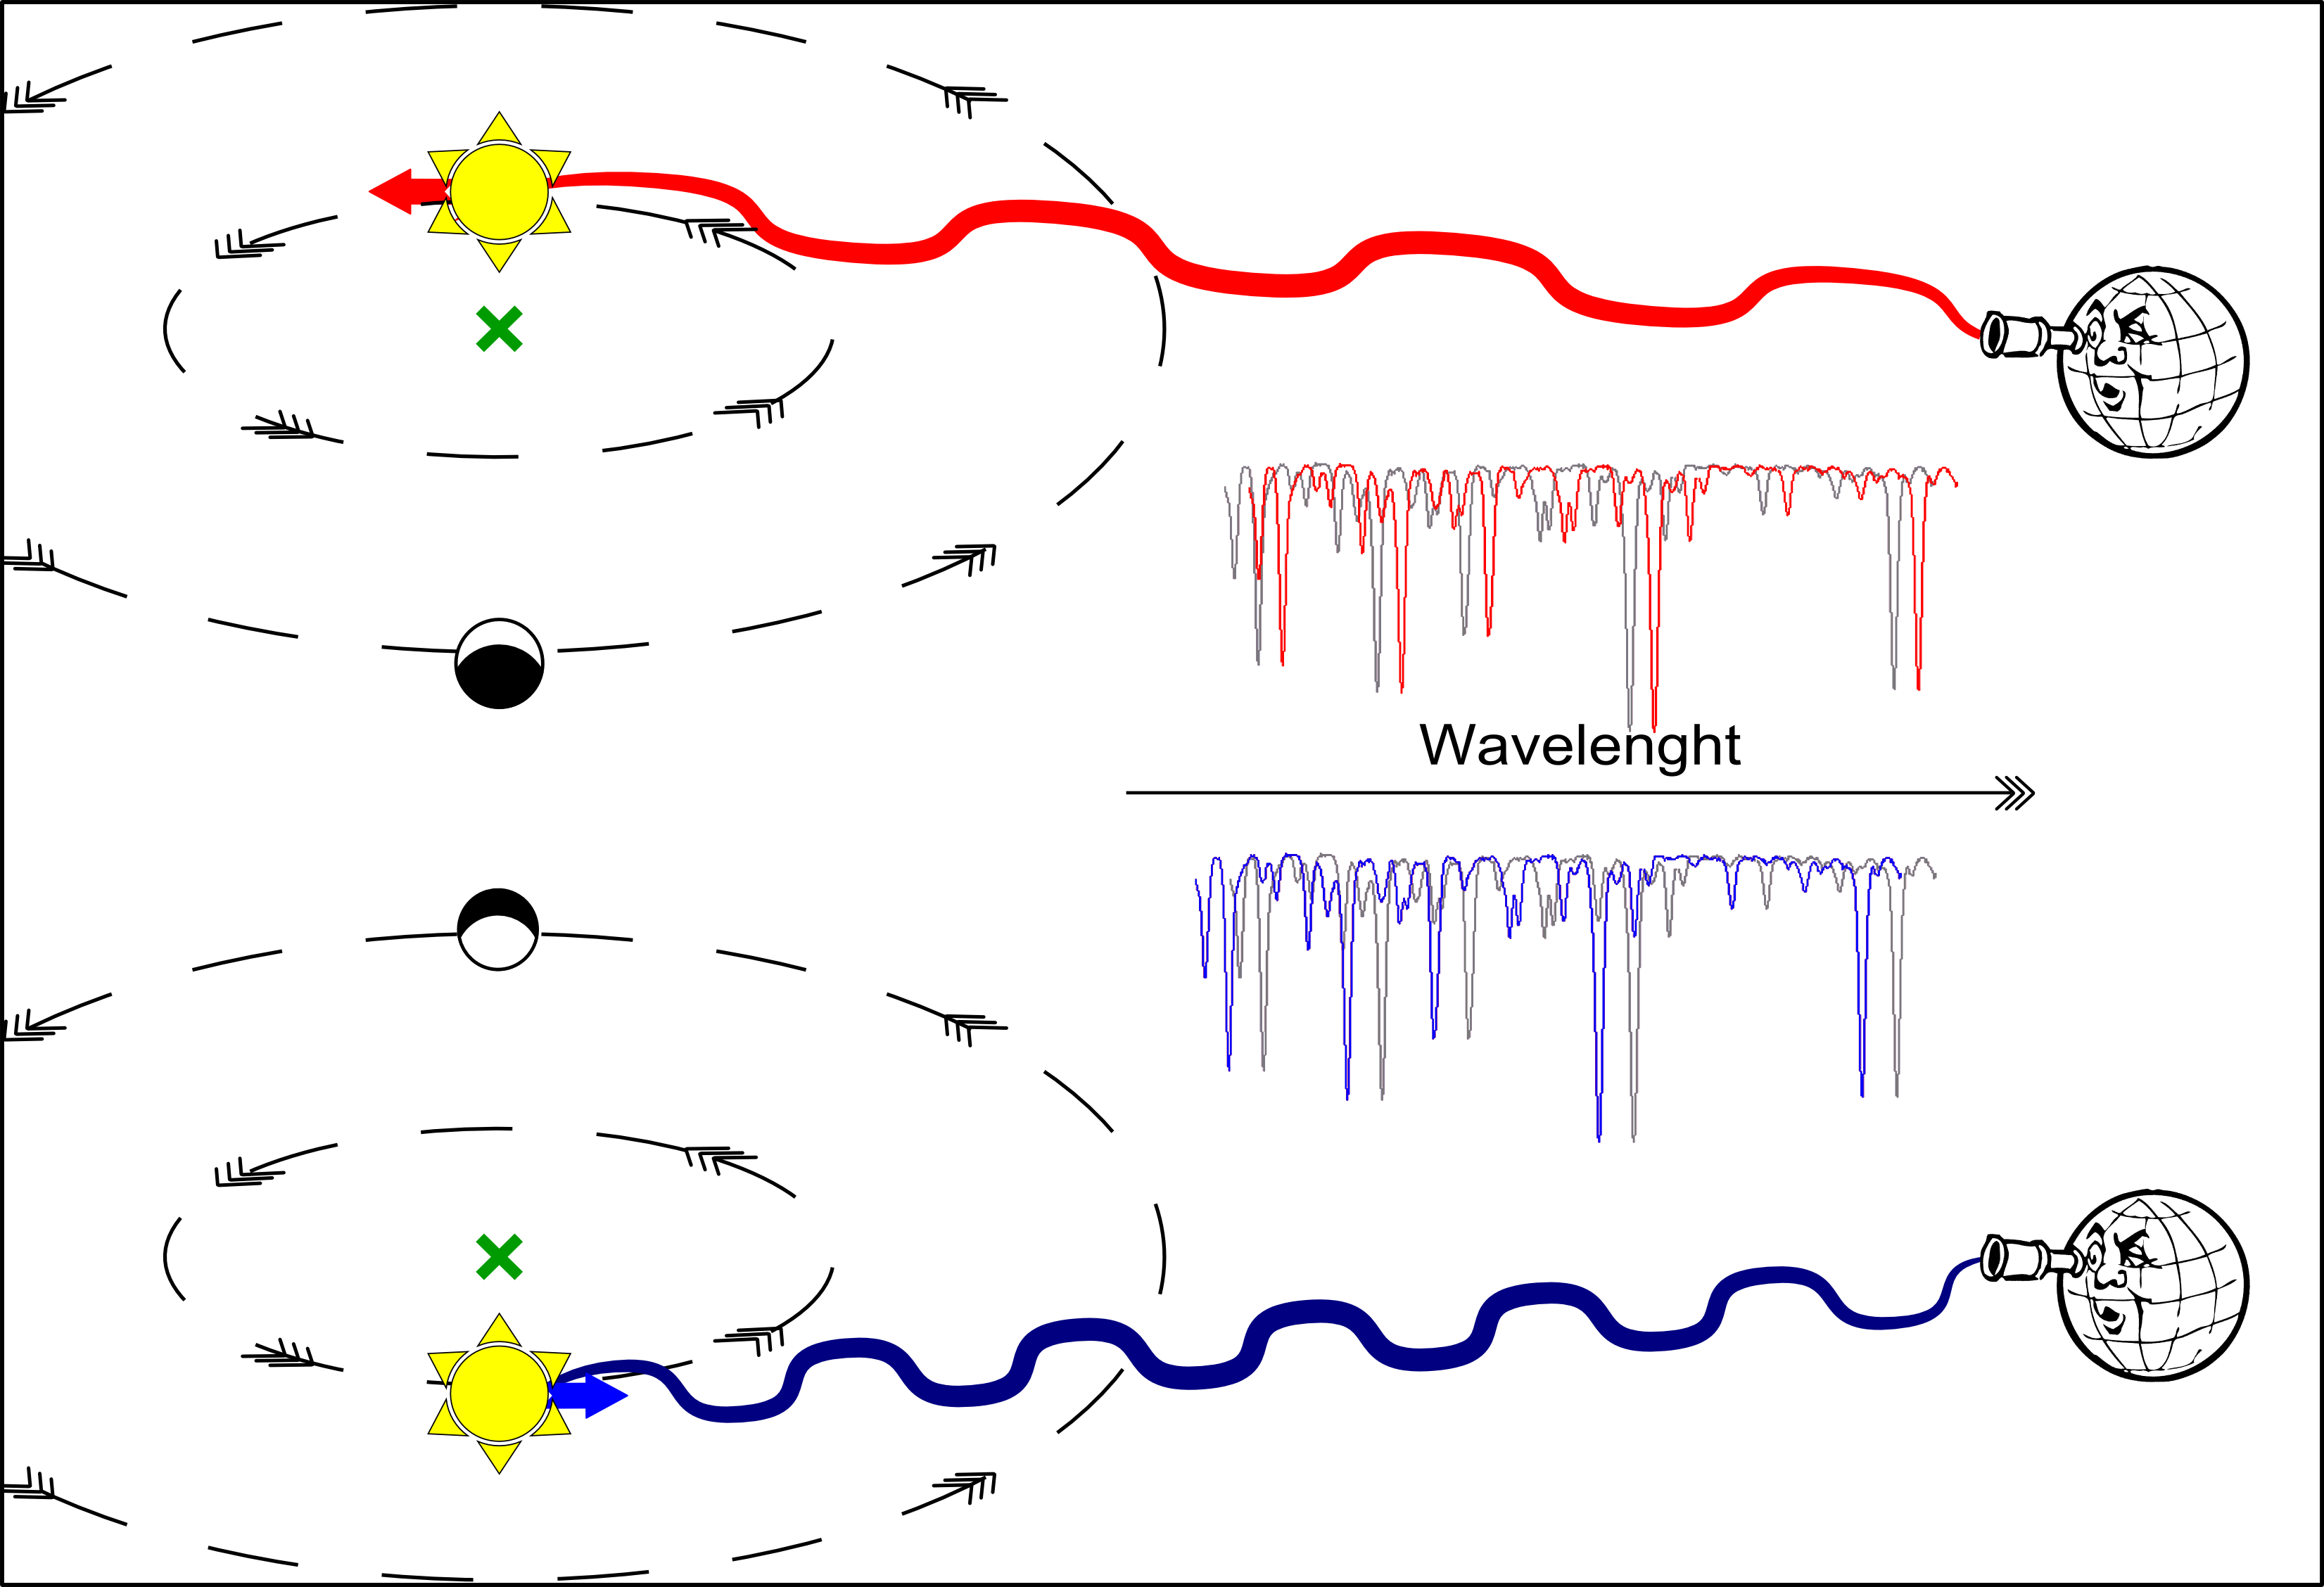
\includegraphics[height=5cm]{./figures/introduction/RV_Diagram}
    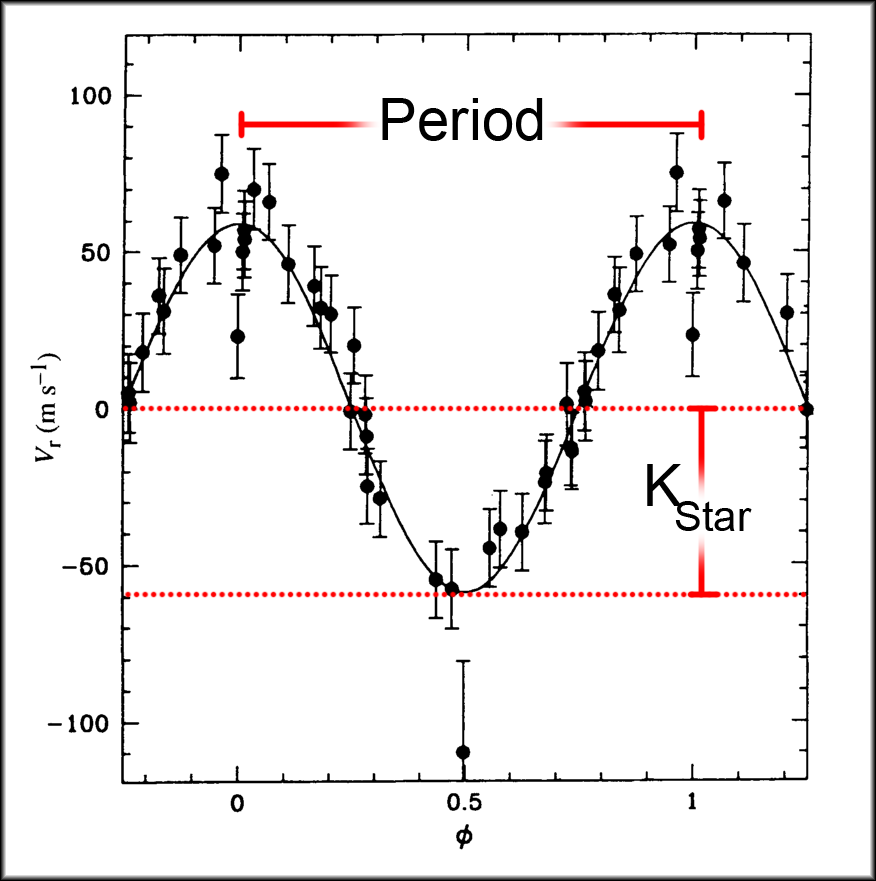
\includegraphics[height=5cm]{./figures/introduction/PhaseFolded_51Pegb_Mayor_et_al_1995}
    \caption[The {RV} method.]{Left: Diagram of {RV} method.
    Right: {RV} variation for the detection of {51 Pegasi}.
    Credit:~\citet{mayor_jupitermass_1995}}.
    \label{fig:rvdiagram-mayor}
\end{figure}

The radial velocity variation, directed along the line of sight, is given by:
\begin{equation}
\label{eqn:rv_equation_intro}
{RV} = \gamma + K [\cos{(\nu(t, P, T_0, e) + \omega)} + e\cos{(\omega)}]
\end{equation}
where \(\gamma\) is constant barycentre velocity of the system relative to the Sun\footnote{Earth's barycentre motion is well known and removed.}, \(K\) is the velocity semi-amplitude, \(e\) the eccentricity, and \(\omega\) is the argument of periastron.
The true anomaly \(\nu\), is a function of time \(t\), orbital period \(P\), and the time of periastron passage \(T_0\), and eccentricity.

The velocity amplitude $K$ of a star of mass $\Mstar$ due to a companion with mass $\Mp$ with orbital period $P$, eccentricity $e$, and inclination\footnote{Relative to a plane that is tangential to the celestial sphere, $i=90$ is edge on.} $i$ is~\citep[e.g.][]{cumming_lick_1999}:
\begin{equation}
    K = {\left(\frac{2\pi G}{P}\right)}^{1/3} \frac{\Mp{} \sin{i}}{{(\Mp{} + \Mstar)}^{2/3}} \frac{1}{\sqrt{1-{e}^{2}}}, \label{eqn:k_amplitude}
\end{equation}
where G is the gravitational constant.

The key exoplanet property determined by the amplitude {RV} technique is the companion mass, relative to the orbital inclination \Mpsini.
As the companion mass is in the numerator of \cref{eqn:k_amplitude} the {RV} technique is more sensitive to larger mass planets.
Also since $K \propto P^{-1/3}$ the amplitude is greater for short period close in orbits\footnote{From Kepler's Law ${P}^{2}\propto {a}^{3}$}.

\begin{figure}
    \centering
    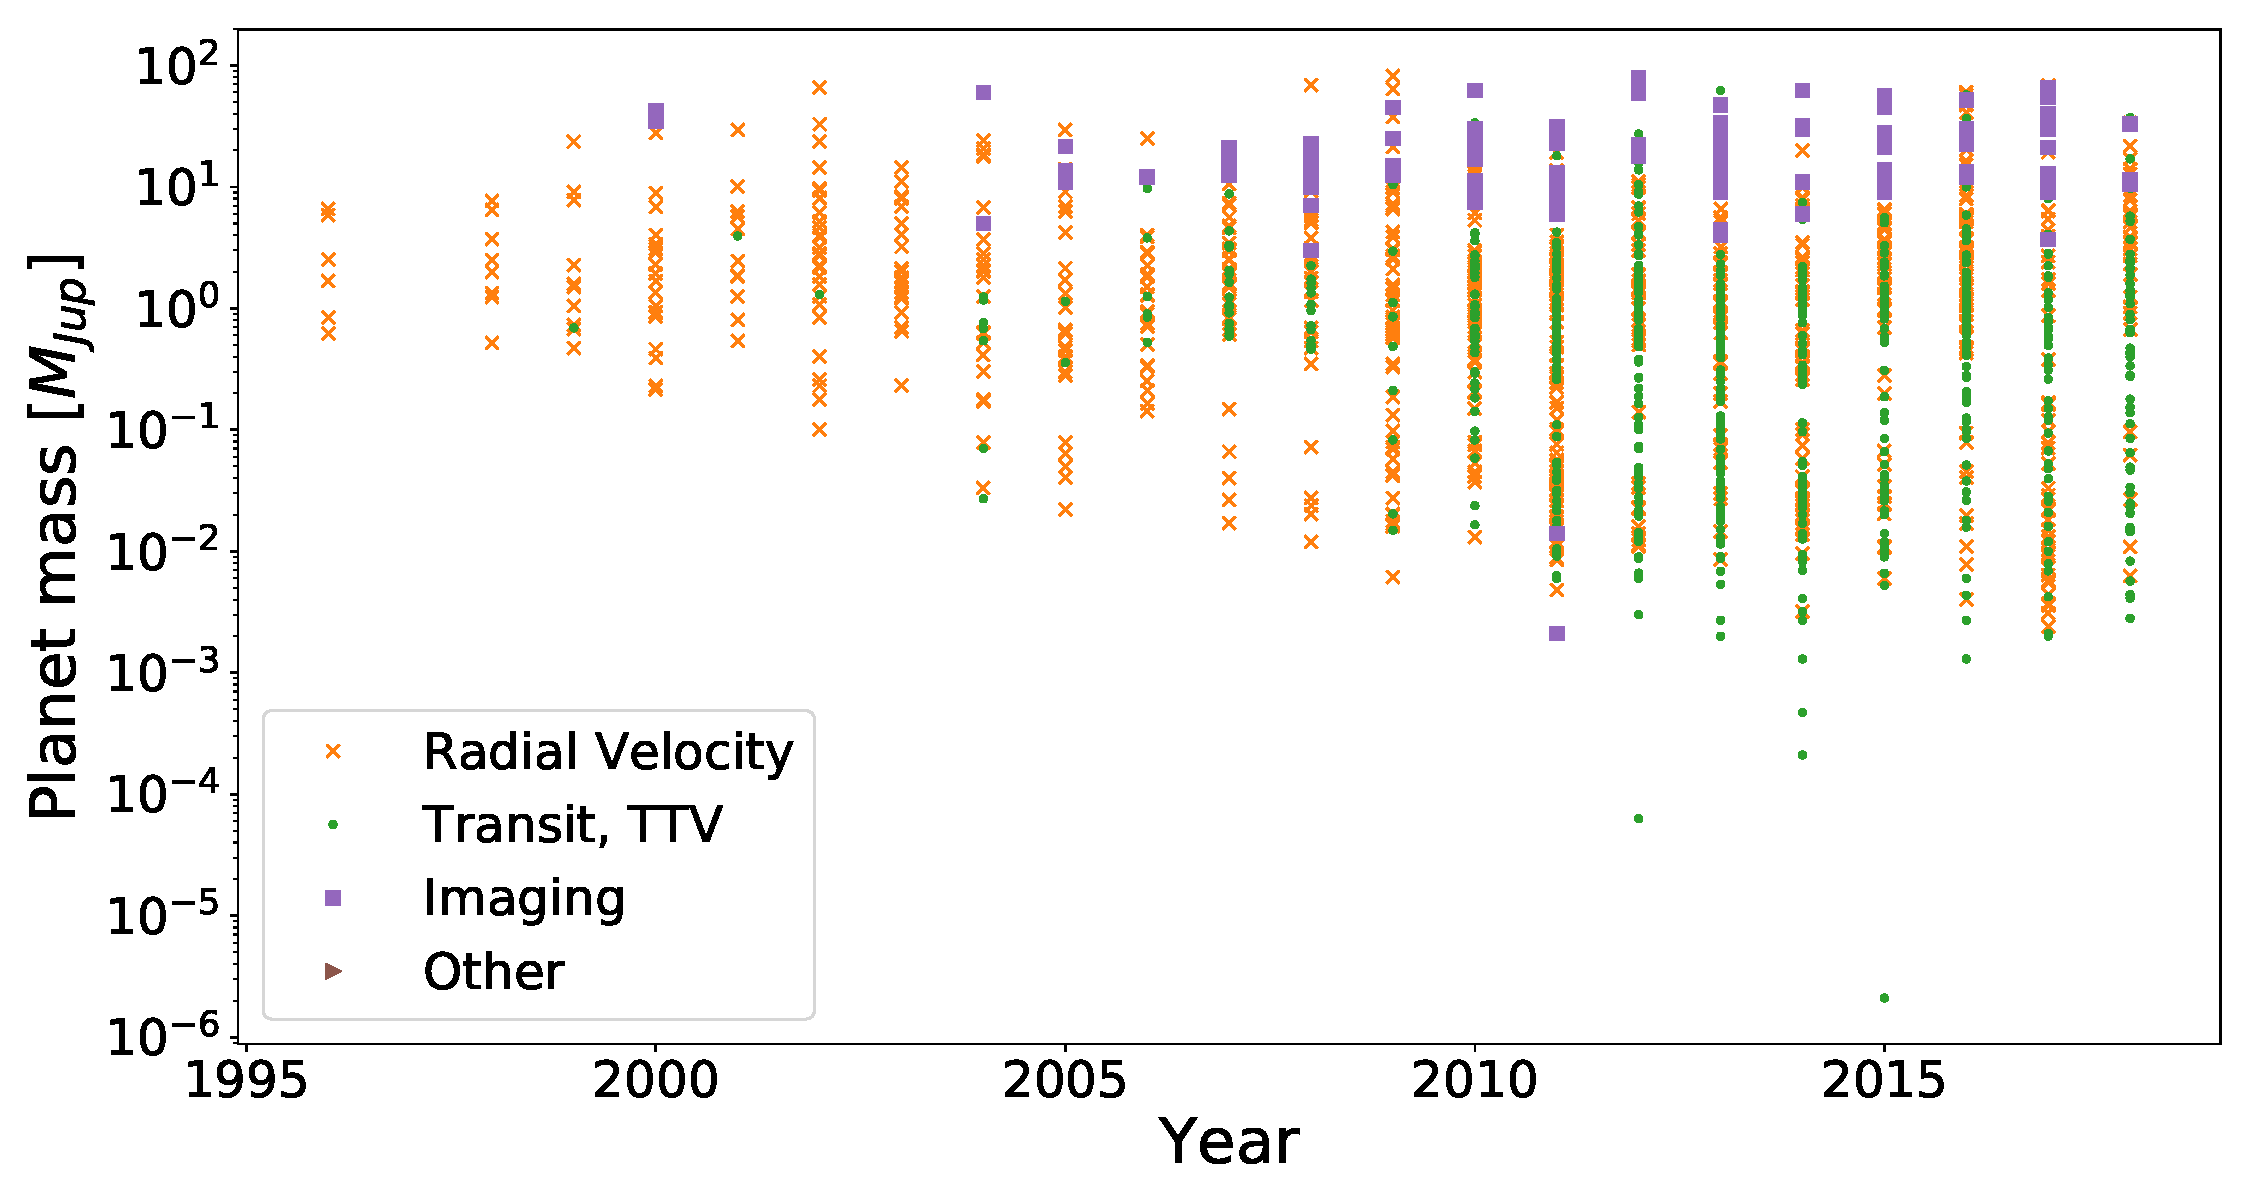
\includegraphics[width=0.7\linewidth]{figures/introduction/exoplanetEU_year_mass.pdf}
    \caption[Exoplanet discovery year verses exoplanet mass.]{Exoplanet discovery year verses exoplanet mass showing a trend towards detecting lower mass planets.
    Exoplanets without a measured mass are not shown.
    The colours indicate the initial detection method.}
    \label{fig:exoplaneteuyearmass}
\end{figure}

The {RV} method kick-started the exoplanet discipline by detecting the first exoplanet around a solar-type star {51 Pegasi}~\citep{mayor_jupitermass_1995}.
The {RV} curve for {51 Pegasi} is shown on the right side of \cref{fig:rvdiagram-mayor}.
The first discoveries were surprising as Jupiter mass planets in short period orbits\footnote{\Mpsini=0.47\,\Mjup{} orbiting at 0.05\AU{} for {51 Pegasi}} were unlike anything in our Solar System and not predicted by standard plant formation theories.
Several exoplanet discoveries followed in quick succession~\citep[e.g.][]{butler_planet_1996, marcy_planetary_1996} with many confirming the existence of the type of planets now referred to as ``hot-Jupiters''~\citep{butler_three_1997, charbonneau_detection_2000}.

The radial velocity amplitudes of the first exoplanets detected were around 60\mps{} while
the radial velocity signal of the Earth in a one year orbit around a solar-type star however is 8.9\cmps{}~\citep[e.g.][]{figueira_radial_2010}.
Dedicated spectrographs, such as HARPS~\citep{mayor_setting_2003} along with improved reduction techniques~\citep{lovis_new_2007} pushed this mass detection limit down to the \mps{} level.
ESPRESSO~\citep{pepe_espresso_2014, megevand_espresso_2014} is the next generation high precision optical spectrograph aiming to push the detection limits to 10\cmps, to detect an Earth twin.
The gradual decrease in measured mass of exoplanets over time is shown in \cref{fig:exoplaneteuyearmass}.
The different symbols indicate the detection method, not necessarily the method used to measure the exoplanet mass.

Most {RV} detection has been performed using optical spectrographs.
However, as the amplitude of {RV} signal is inversely proportional to the mass of the star (RV $\propto \Mstar^{-2/3}$), there are dedicated surveys focusing on smaller mass M-dwarf stars~\citep[e.g.][]{reiners_carmenes_2018}.
M-dwarfs are inherently cooler and thus emit a majority of their stellar output in the near-infrared.
New dedicated high-resolution \nir{} spectrographs have and are being designed and implemented to meet this demand e.g.\ {CARMENES}, {NIRPS}, {SPIRou}, {CRIRES+}.


\subsection{Transit methods}
\label{subsec:transit}
The transit method detects the presence of an exoplanet by observing the periodic dimming of the star due to the passage of the exoplanet between the star and observer, partially blocking the star.
Geometry requires the orbit of the exoplanet to be aligned edge-on to the line of sight (low inclinations) for a transit to occur.
The geometric probability, $P$, that a exoplanet transits is estimated by
\begin{equation}
P \approx \frac{\Rstar}{a (1-{e}^{2})},
\end{equation}
where \(e\) is the eccentricity of the orbit, $\Rstar$ is the star radii and \(a\) is the semi-major axis of the orbit (star-planet distance)~\citep[e.g.][]{barnes_effects_2007}.
The probability of transit increases with the size of the star but decreases with distance to the star.

The drop in stellar brightness during the transit allows the measurement of the planet/star radius ratio:
\begin{equation}
    \frac{\Delta L}{L}\sim{\left(\frac{\Rp}{\Rstar}\right)}^{2}
\end{equation}
where \(L\) is the luminosity of the star, \(\Delta L\) is the maximum luminosity variation (transit depth), and \(\Rstar\) and \(\Rp\) are the radius of the star and planet respectively.

The transit method complements {RV} measurements as the inclination, $i$, of the orbit can be determined from the transit.
This removes the {$\sin{i}$} ambiguity found in the \Mpsini{} of {RV} detections so the true mass, $\Mp$, of the exoplanet can be revealed.
The true mass along with the planet's radius provides a value for the exoplanets average density\footnote{$\rho \equiv \frac{\textrm{Mass}}{\textrm{Volume}} = \frac{3}{4\pi}\frac{\Mp}{\Rp^{3}}$}, hinting at the possible composition.

There are several other astrophysical phenomena which can mimic transiting exoplanet signals, created by configurations of two or more stars which may not involve an exoplanet.
For example a transiting low-mass or white-dwarf star, grazing binary stars, or a transit in a multi-star system~\citep[see e.g.][]{cameron_extrasolar_2012, santerne_contribution_2013}.
Follow-up {RV} observations~\citep[e.g.][]{santerne_radial_2011} are usually required to confirm the planets existence.
Statistical validation techniques are also possible, such as the PASTIS software~\citep{diaz_pastis_2014}, when follow-up can not be performed.
These techniques assess the likelihood of the planet being a true planet against the different false positive scenarios, validating or confirming the planet if the likelihood is high enough.

The transit method has the highest false positive rate among the detection methods presented here.
With {RV} follow-up,~\citet{santerne_sophie_2012} found a false positive rate as high as 35\% for short period giant planets, while~\citet{santerne_sophie_2016} found a 54.6\% false positive rate of 129 giant planets with periods less than 400 days.
These sub-sample false positive rates are however higher than the global false positive rate of 9.4\%~\citep{fressin_false_2013}/11.3\%~\citep{santerne_contribution_2013} found for Kepler.
Some of the currently known exoplanet systems with the smallest radii and lightest mass have been detected through transit and later confirmed with high-precision {RV} follow-up~\citep[e.g.][]{queloz_corot7_2009, pepe_earthsized_2013, lopez-morales_kepler21b_2016, ment_second_2018}.

The identification of unresolved multiple stars, such as a binary or an unrelated background star, can be achieved through high-resolution spectroscopy in which the spectral lines of individual stars can be separated~\citep{kolbl_detection_2015}.
This is important to measure the correct radii of exoplanets as the extra light contribution from an unresolved secondary star will reduce the transit depth, mimicking a smaller transiting planet.

The transit of a single planet can not directly determine the planetary mass.
However, in multiple planet systems, the masses and sometimes the presence of other planets in the system can be determined from perturbations in the transit time and duration~\citep[e.g.][]{holman_use_2005, holman_kepler9_2010}.
A large number of systems have been detected that show transit timing variations (TTV) and transit duration variations (TDV)~\citep[e.g.][]{holczer_transit_2016} due to the gravitational interaction between planets.
The statistical validity of multi-transiting planets is more straightforward than single planets as the probability of having multiple false positives, being the product of the individual probabilities, is lower than having multiple planets in the system~\citep{lissauer_almost_2012}, making multiple planet systems easier to validate.

The presence of star spots on the surface of a star can be observed during transit.
A star spot is a dark region on the stellar surface due to magnetic fields, which decreases the luminosity slightly.
Examples of spots can be seen in the middle of the Sun from an image of the 2012 transit of Venus in \cref{fig:transit_venus_transit_alignment} (left).
It shows several dark sunspots alongside Venus, although Venus did not cross them.
Unlike for other stars, sunspots are spatially resolved.
If an exoplanet passes in front of a spot, the luminosity decrease from the spot is temporarily hidden and a small bump occurs in the transit shape.
The presence of spots in successive transits (see \cref{fig:transit_venus_transit_alignment} (right)) can indicate the alignment of the stellar rotation to the planet orbital plane~\citep{sanchis-ojeda_starspots_2013}.
In this simulation an orbit aligned with the stellar rotation and the transit crosses the spot in four successive orbits.
In a misaligned case a spot would only be observed in one transit.

\begin{figure}
    \centering
    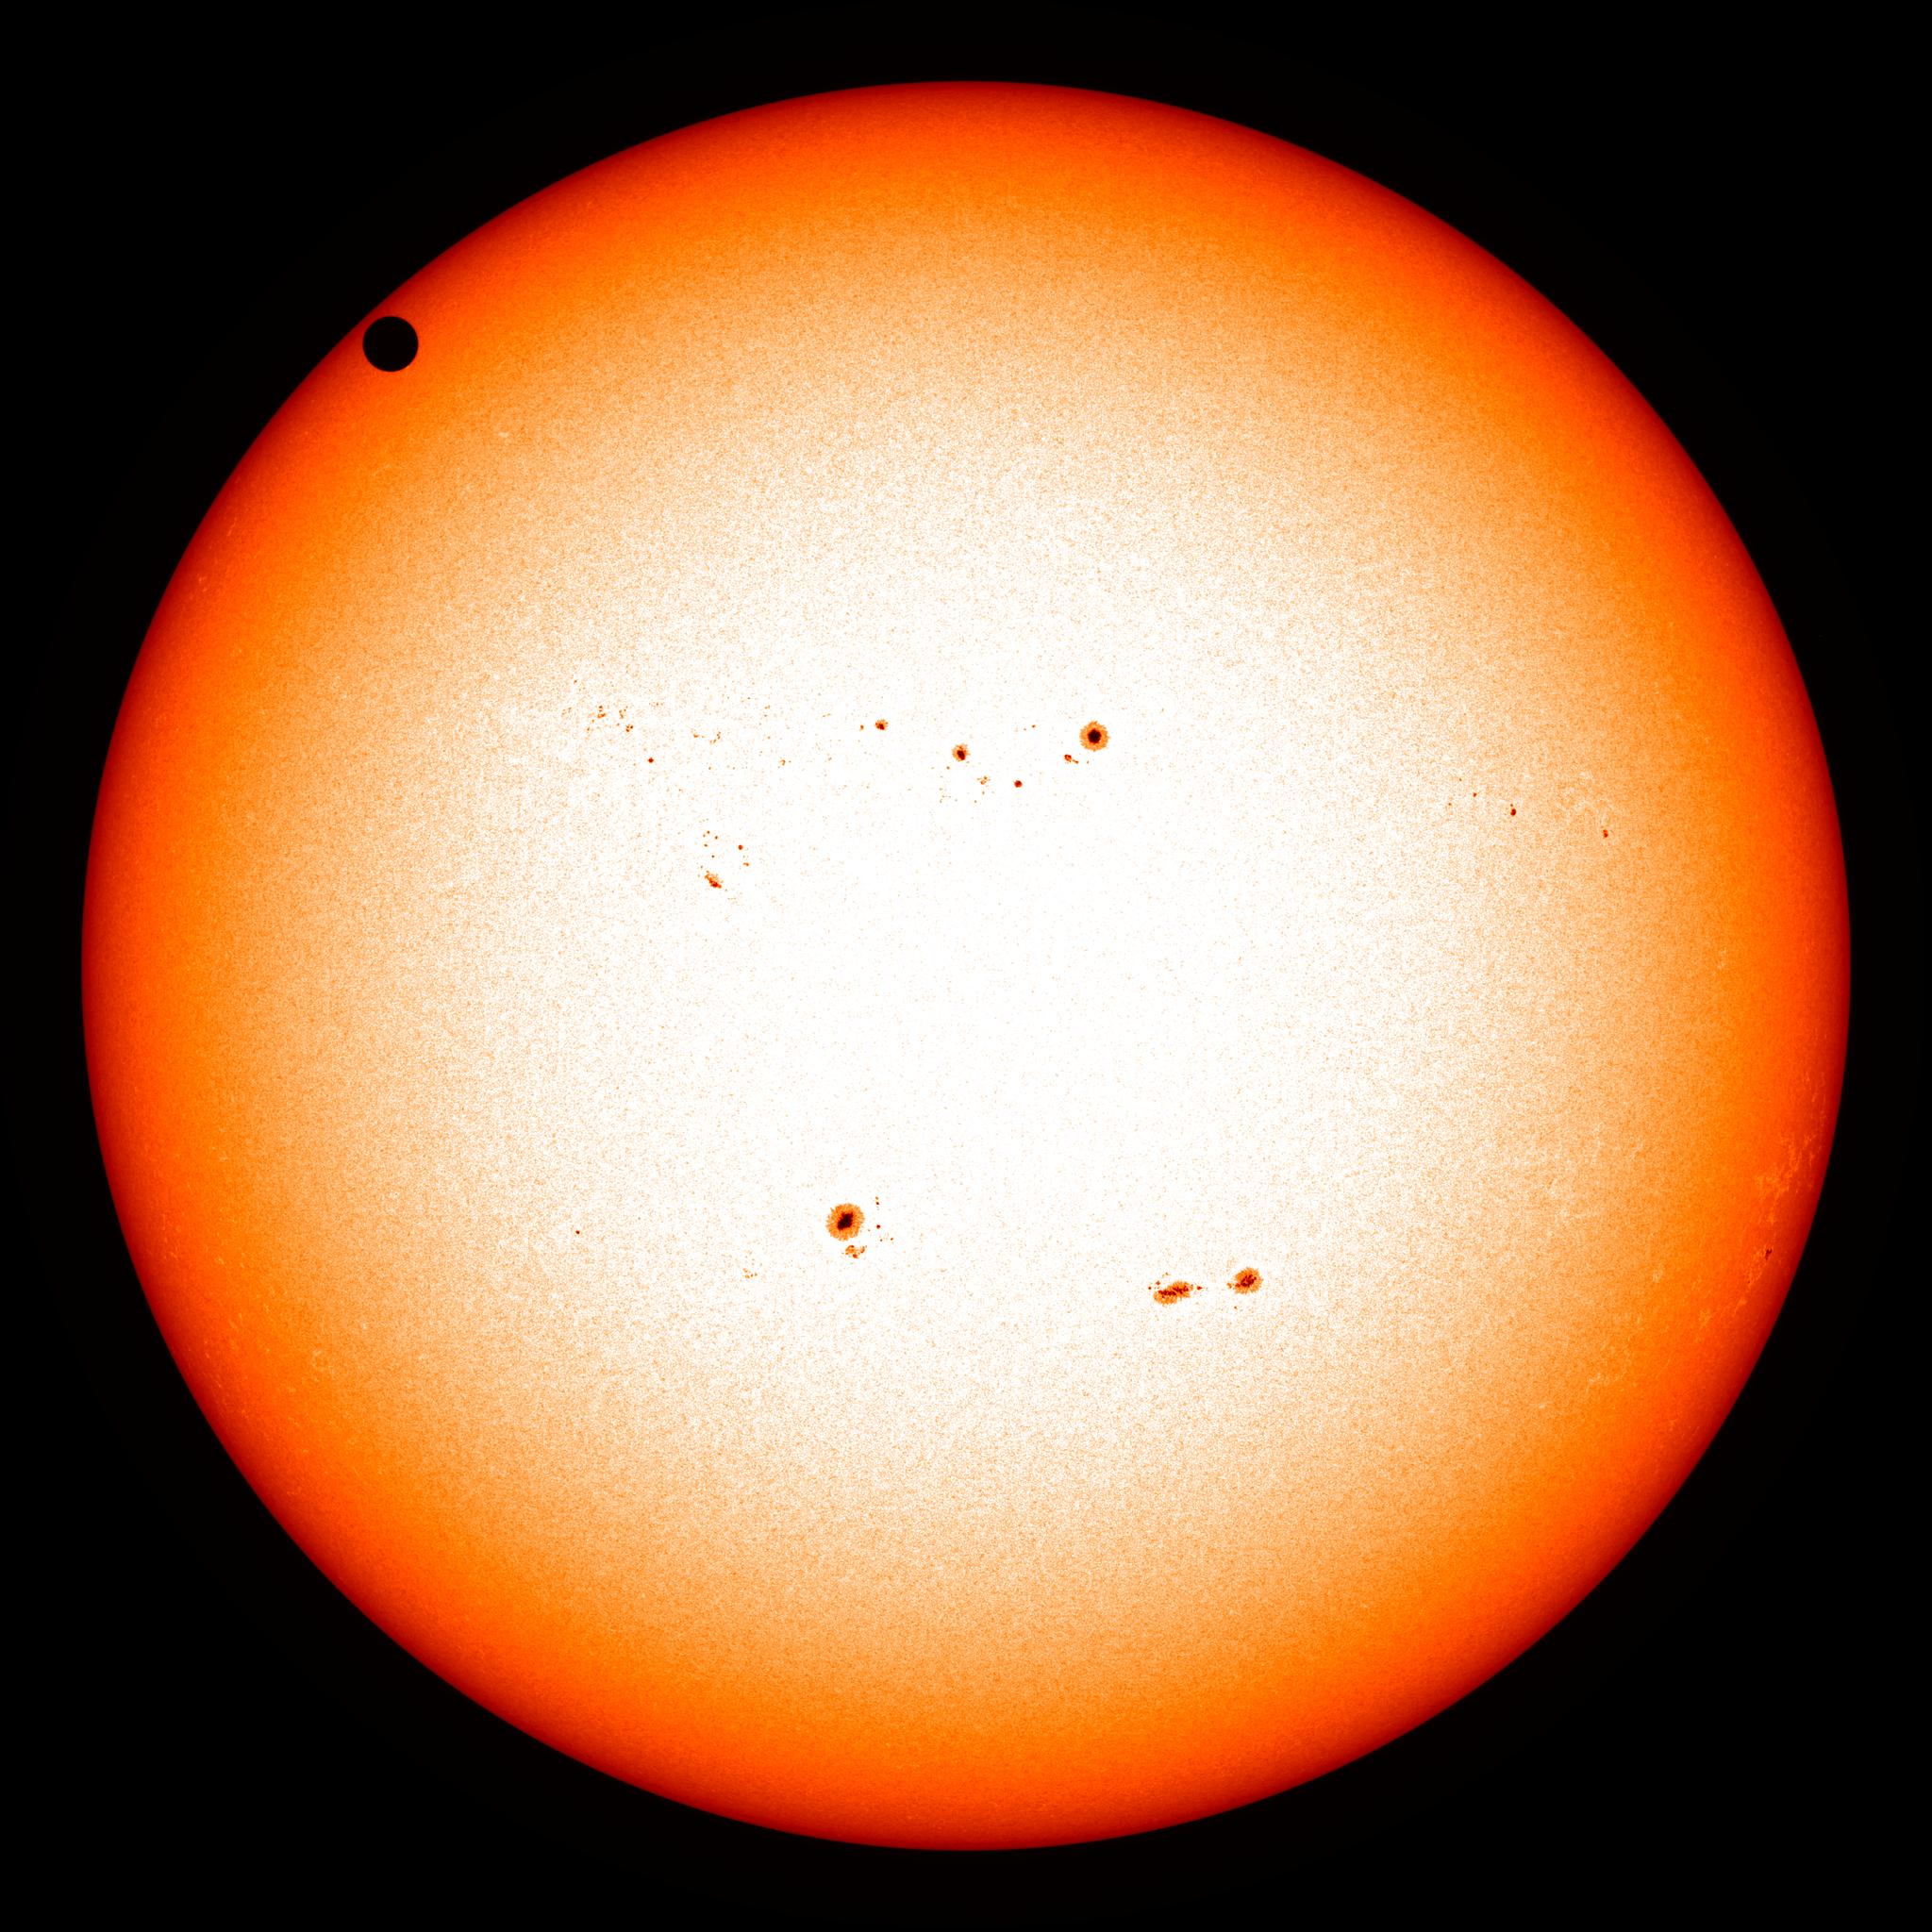
\includegraphics[height=5cm]{./figures/introduction/SDO_2012_Venus_Transit.jpg}
    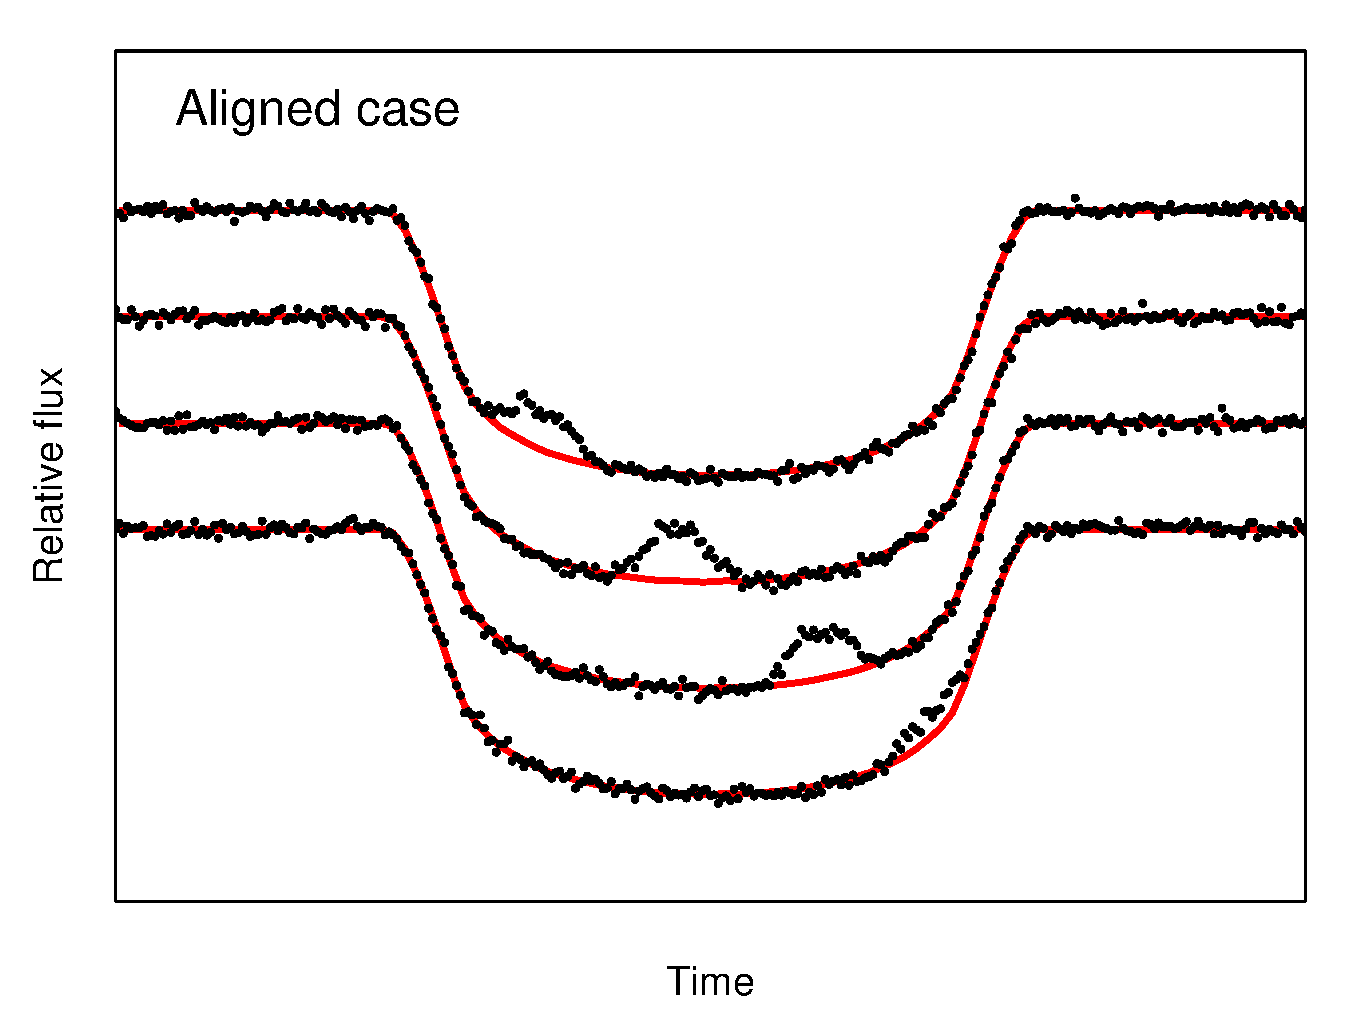
\includegraphics[height=5cm]{figures/introduction/sanchisojedafig1-crop.pdf}
    \caption[Transit of Venus and successive transit corssings.]{Left: Image from the 2012 transit of Venus obtained from the Solar Dynamics Observatory satellite.
    Venus is the dark circle in the top left of the Sun.
    Limb darkening is observed as the change in colour/brightness from white to red near the edge.
    Several sunspots are also observed on the surface of the Sun.
    Credit: {NASA}/{SDO}, {HMIR}.
    Right: Simulation of 4 successive transits crossing a star spot with the orbit aligned with the stellar rotation.
    The stellar rotation is 1/10 the orbital period.
    Adapted from~\citet[][Figure~1]{sanchis-ojeda_starspots_2013}.}
    \label{fig:transit_venus_transit_alignment}
\end{figure}


The vast majority of transit detections have come from Kepler~\citep{borucki_characteristics_2011}, which focused on a small patch of sky (0.25\%) for four years continuously.
Kepler's impressive sensitivity compared to previous surveys, allowed it to detect planets down to around 2\Rearth.
However, {CoRoT}~\citep{barge_transiting_2008} and ground-based surveys, such as WASP~\citep{pollacco_wasp_2006}, OGLE~\citep{udalski_optical_2002}, TreS~\citep{alonso_tres1_2004} have also had successful transit detections.

Following in Kepler's footsteps the next generation transit hunter {TESS}~\citep{ricker_transiting_2015} has already announced discoveries of new transiting planets only months after launch~\citep{vanderspek_tess_2018, gandolfi_tess_2018, huang_tess_2018}.
It will eventually cover more than 90\% of the sky with an impressive planetary yield expected of $\sim10\,000$ exoplanets, with around 3500 the size of Neptune or smaller~\citep{barclay_revised_2018, huang_expected_2018}.
However, the observation coverage is not uniform, with the majority of the ecliptic plane receiving only one month of observations, limiting the detection sensitivity to short period transiting planets.
On the other hand, the ecliptic poles will receive almost one year continuous observation.

{PLATO} \citep{rauer_the_2014} is another transit survey mission planned for launch in 2026.
In contrast to Kepler it will focus on brighter nearby, stars, with the goal to detect and accurately determine the planetary parameters of Earth-like planets in the habitable zone.

A smaller transiting mission, {CHEOPS} \citep{broeg_cheops_2013}, is also scheduled for launch at the end of 2019.
Unlike the transiting surveys mentioned above, {CHEOPS} will perform dedicated transit follow-up of bright stars with known planets, such as those found with {RV} surveys.
It will providing high precision transit photometry, if the geometry allows, to obtain precise planetary radii.


\subsection{Direct Imaging}
\label{subsec:direct_detection}
The direct imaging technique involves directly imaging an exoplanet in orbit around a star.
The first planets directly imaged were {2MASSWJ~1207334--393254~b} using adaptive optics with NACO on the VLT~\citep{chauvin_giant_2004}, three planets around HR\,8799 using angular differential imaging on the Keck and Gemini telescopes~\citep{marois_direct_2008}, and {Fomalhaut~b} using chronography on the HST~\citep{kalas_optical_2008}.
As an example, the direct image of {HR\,8799} is shown in \cref{fig:directimaging}, where a fourth planet was revealed~\citep{marois_images_2010}.

Direct imaging requires resolving the angular separation between the star and planet and is best suited to detect giant planets in wide orbits (>10\AU{}) around nearby stars.
This is shown by the clustering of direct image detections shown in \cref{fig:exoplaneteuyearmass}.
Extremely young giants observed in the infrared are favoured as they have higher thermal emissions (while they are still cooling) and larger surface area resulting in a higher contrast ratio to the host.


\begin{figure}
    \centering
    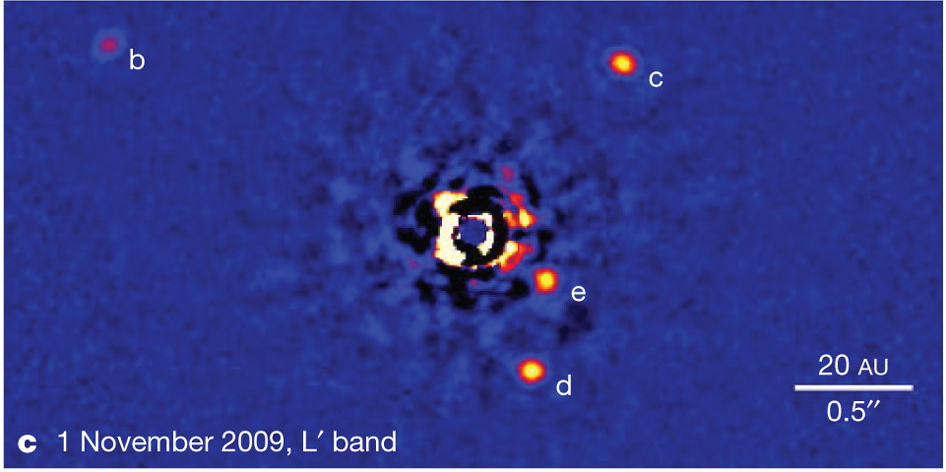
\includegraphics[width=0.5\linewidth]{./figures/introduction/DirectImaging_HR8799_MaroisEtAl2010}
    \caption[Direct detection of four exoplanets around HR\,8799.]{Direct detection of four exoplanets around HR\,8799~\citep{marois_images_2010}.}
    \label{fig:directimaging}
\end{figure}

High-contrast adaptive optics instruments, such as SPHERE@VLT~\citep{beuzit_sphere_2008} and GPI~\citep{macintosh_gemini_2008}, are being used with several different techniques to observe targets closer to the star and with smaller contrasts, usually involving blocking or cancelling out the light from the star while retaining the signal of the planet~\citep[e.g.][]{marois_direct_2005, mawet_annular_2005, schmid_zimpol_2005, sirbu_prospects_2017, sirbu_techniques_2017, wang_observing_2017}.
Ground based direct imaging requires adaptive optics to reduce the turbulence induced by the atmosphere, increasing the angular resolution down to the telescope diffraction limit.

On top of hardware based solution to the stellar contamination, cleaver observing strategies and cancelling algorithms.
Angular differential imaging (ADI) \citep[eg.][]{marois_direct_2005} is one such technique.
ADI, disables the field de-rotator component in the telescope so that the viewing field rotates relative to the plane of the detector during the night.
Several images taken at different angles are rotated to a reference position and stacked.
The stacking of images from different angles cancels out the pseudo-static speckle caused by the telescope and optics while increasing the contrast of any faint object in the stars vicinity, i.e. a planetary companion.

The direct imaging technique is also used to observe circumstellar and protoplanetary disks, and has even captured images of planets during formation~\citep[e.g.][]{sallum_accreting_2015}.
Combining direct images from different photometric bands can allow for the creation of low-resolution exoplanet spectra~\citep[e.g.][]{kuzuhara_direct_2013, zurlo_new_2015}.


\subsection{Astrometry}

\label{subsec:astrometry}
Astrometry measures the precise position of the stars on the plane of the sky.
The motion of a star with an exoplanet about its centre of mass can be observed in the periodic oscillating of position from its proper motion in the sky.

For a circular orbit the angle of the semi-major axis of the apparent orbital ellipse, the amplitude of the astrometric signature ($\theta$), is given by
\begin{equation}
\theta = \frac{M_{p}}{M_{star} + M_{p}} \frac{a}{d}
\end{equation}
where, $\Mp$ and $\Mstar$ are the planet and stellar mass, $a$ is the semi-major axis (in \AU) and $d$ is the distance from the observer to the system (in parsec)~\citep{perryman_exoplanet_2011}.

This shows that the astrometric signal is proportional to the companion/star mass ratio and to the orbital radius, $a$.
The amplitude also decreases inversely with distance, as the angles become smaller.
This is unlike the {RV} and transit methods for which the amplitude is not affected by distance.
Astrometry is complementary to the {RV} method as it measures the orbital motion perpendicularly to the line of sight, allowing the three-dimensional orbit to be determined.

A modelled astrometric signal is shown in \cref{fig:astrometry_perryman}, for a star at a distance of 50\pc, with a proper motion of 50\masperyr{}, and orbited by a planet of $\Mp = 15$\,\Mjup{}, $e = 0.2$, and $a = 0.6$\AU~\citep{perryman_extrasolar_2000}.
The straight dashed line shows the path of the system's barycentric motion viewed from the Solar System barycentre.
The dotted line shows the effect of parallax (the Earth's orbital motion around the Sun, with a period of 1 year).
The solid line shows the apparent motion of the star as a result of the planet, the additional perturbation being magnified by $\times 30$ for visibility.

Although astrometry has detected many binary stars~\citep[e.g.][]{gontcharov_new_2000} and found several brown-dwarf companions~\citep[e.g.][]{sahlmann_search_2011}, the exoplanet discovery's are few.
A 1.5\,\Mjup{} mass planet in a roughly 1000 day orbit around {HD\,176051} was reported by~\citet{muterspaugh_phases_2010}, and recently the astrometric perturbation of a known planet, {Beta Pictoris~b}, was performed utilizing measurements from {GAIA}~\citep{collaboration_gaia_2016a} and {HIPPARCOS}~\citep{esa_hipparcos_1997} to determine a mass of 11\,\Mjup~\citep{snellen_mass_2018}.

The predicted astrometric variations for an exoplanet are at the level of sub-milliarcseconds and therefore are not achievable from the ground due to atmospheric turbulence.
The most precise astrometric measurements come from spacecraft.
These are currently being performed using GAIA with the recent release of astrometric parameters for 1332~million sources~\citep{collaboration_gaia_2018} and reaching a precision of 0.04\,mas for the brightest stars (<14 magnitude).
Simulations predict that more than 21\,000 large mass planets (1--15\,\Mjup) in long-period orbits should be discovered during the 5 year nominal GAIA mission~\citep{perryman_astrometric_2014}.

\begin{figure}
    \centering
    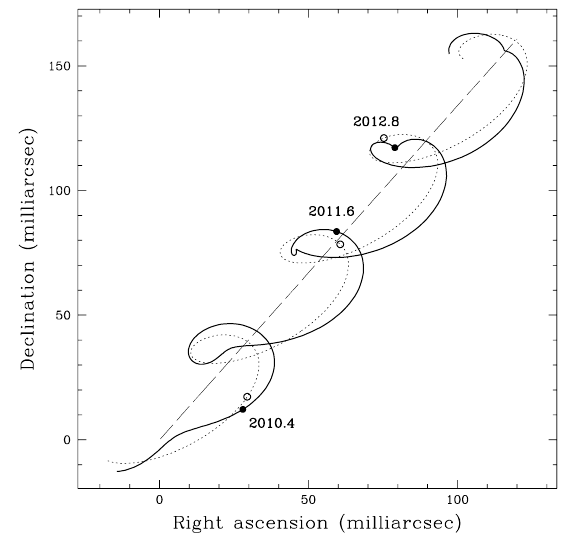
\includegraphics[width=0.5\linewidth]{./figures/introduction/Astrometry_Perryman2000.png}
    \caption[Modelled astrometric path on the sky.]{The modelled astrometric path on the sky from~\citet{perryman_extrasolar_2000}.
    Showing a star at a distance of 50\pc, with a proper motion of 50\masperyr{}, and orbited by a planet of $\Mp$ = 15\,\Mjup{}, $e$ = 0.2, and $a$ = 0.6\AU{}.
    The straight dashed line shows the path of the system's barycentric motion viewed from the Solar System barycentre.
    The dotted line shows the effect of parallax (the Earth's orbital motion around the Sun, with a period of 1 year).
    The solid line shows the apparent motion of the star as a result of the planet, the additional perturbation being magnified by $\times 30$ for visibility.}
    \label{fig:astrometry_perryman}
\end{figure}


\subsection{Microlensing}
\label{subsec:microlensing}
Microlensing is an astronomical effect predicted by Einstein's General Theory of Relativity.
The mass of an object bends space-time which causes light to be visibly deflected around large mass objects.
As a star passes between Earth and a distant star it acts like a lens, bending and magnifying the light from the background star.
The gravitation of a planet orbiting the lens star (if it exists) creates a distortion in the lens, leading to small caustics, deviations in the microlensing light curve for a single lens event (star without a planet).

An example is shown in \cref{fig:microlensing_example} where a lensing magnification of up to $\times3$ is observed for {OGLE2005-BLG-390}~\citep{beaulieu_discovery_2006}.
On the falling edge of the lensing event (and inset top right) there is a bump due to the presence of a 5.5\,\Mjup{} companion.

The difficulties of microlensing is that they require the chance alignment between Earth, a nearby lens star, and a distance source star, which is unrepeatable.
Some caustics are often difficult to fit and yield degenerate results, making characterization of the planet difficult.
Follow-up measurements of a handful of microlensing events have been performed~\citep[e.g.][]{kubas_frozen_2012, batista_confirmation_2015, santerne_spectroscopic_2016} to break degeneracies.
However, follow-up can be difficult as microlensing is sensitive to distant host stars, which are outside the ability of current spectrographs.
It is also sensitive to planets with a wider orbital separation compared to transits and {RV}.
Currently there are 87 planets in 82 systems detected by microlensing, as listed in the \href{https:\\www.exoplanet.eu}{exoplanet.eu} database.

The microlensing technique has been efficient in detecting Neptune analogue planets, distant planets similar in size to Neptune.
Showing that cold Neptune planets are likely most common pe of planet outside of the snow line \citep{suzuki_exoplanet_2016}, the distance from the star at which point it is cold enough for volatile compounds (e.g.\ \ce{H20}, \ce{NH3}, \ce{CO2}) to condense into solid ice grains.

Microlensing events are detected and monitored using dedicated global telescope networks such as {OGLE}, {MOA}, {microFUN} and {PLANET}.
They focus their viewing towards the galactic bulge where there are more stars and a higher chance for microlensing events to occur.

The precise stellar proper motions from the GAIA mission are being used to predict possible future alignments that could produce microlensing events~\citep{kluter_prediction_2018}

\begin{figure}
    \centering
    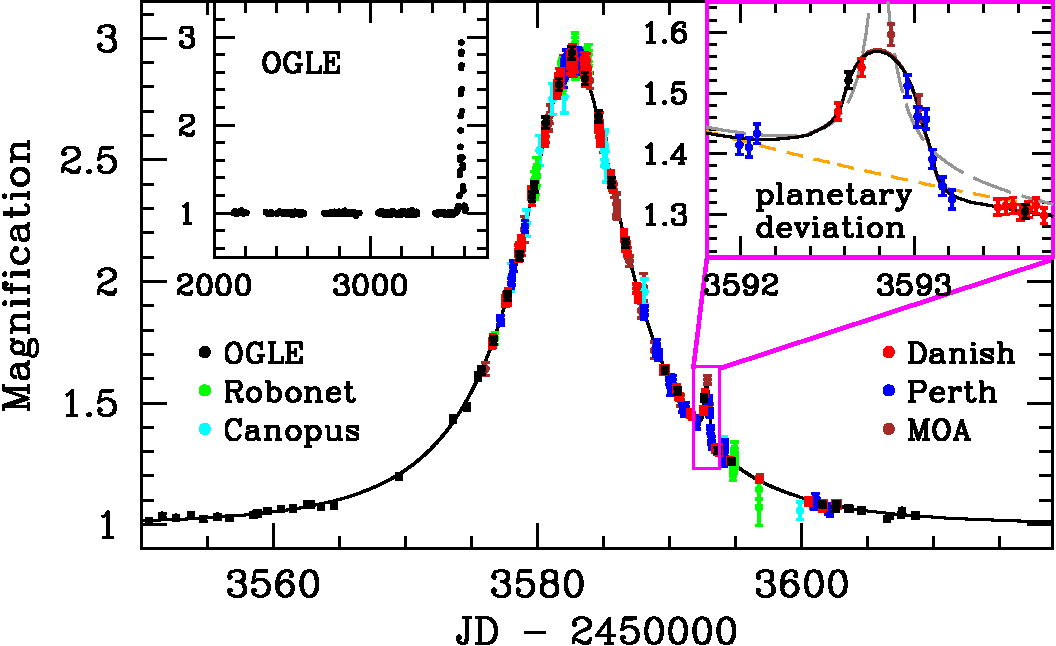
\includegraphics[width=0.5\linewidth]{./figures/introduction/Microlensing_OGLE2005-BLG-390.pdf}
    \caption[Microlensing magnification of OGLE2005-BLG-390.]{Microlensing magnification of OGLE2005-BLG-390 from~\citep{beaulieu_discovery_2006}.
    The presence of the 5.5\,\Mjup{} planet causes the small bump shown in the upper right inset plot.}
    \label{fig:microlensing_example}
\end{figure}

\subsection{Pulsar timing}
\label{subsec:pulsar_timing}
Pulsars are rapidly rotating neutron stars or white dwarfs formed after the death of a giant star, that radiate an intense electromagnetic beam.
The timing variations of the millisecond pulsar\footnote{Rotating at 9\,650 revolutions per minute} {PSR1257+12} led to the first extrasolar planet detection~\citep{wolszczan_planetary_1992}.
There are two models of planet formation around pulsars: either they formed before the supernova explosion and survived, or they formed after, from the remnants of the supernova~\citep{starovoit_existence_2017}.
There is still a rarity of less than 10 pulsars with known orbiting planets.

The rarity of these events is partially associated to the technique which requires very precise instrumentation on high cadence (< milliseconds) to precisely measure the electromagnetic radiation from the pulsar.
For example the first pulsar was detected with the Arecibo radio telescope.
With the primary dish fixed into the mountain, its pointing is limited and achieved by moving the receiver.
It has a limited number of stars that can be observed with a sufficient time coverage to detect planets around pulsars.



%!TEX root = ../../thesis.tex

\section{Detecting atmospheres}
\label{sec:decting_atmopsheres}
To help characterize an exoplanet, a detection of its atmosphere can provide useful information.
After the detection of exoplanets and the measurement of their bulk properties, detecting their atmospheres is the next step.
The detection of planetary atmosphere is difficult due to the low planet-to-star flux ratio.
This requires high precision instrumentation to detect.
For example the planet-to-star flux ratio in the optical is $\approx 10^{-4}$ for a hot Jupiter with a 3 day orbit, in which the main component is reflected star light.
In the infrared the thermal emission of the planet dominates and the flux ratio rises to $\approx 10^{-3}$.
These flux ratios requires observations with signal-to-noise ratios of $10^4$ and $10^3$ in the optical and infrared respectively to achieve a planetary signal at the same level as the noise level.
These detections are only just at the capabilities of the current generation of technology, and with very long observation cost.

Several photometric and high-resolution spectroscopic techniques are showing promising results; these are detailed in the following sections.


\subsection{Occultation and phase variations}
\label{subsec:phase_variation}

\begin{figure}
    \centering
    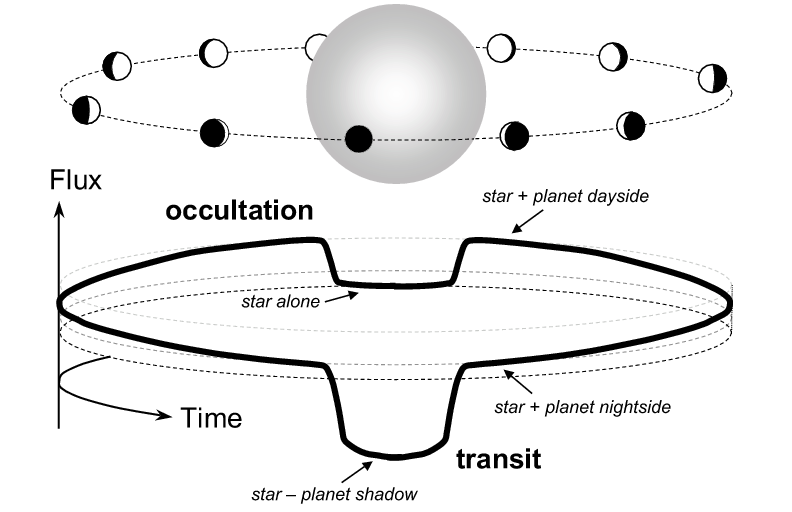
\includegraphics[width=0.6\linewidth]{./figures/introduction/circular_diagram.png}
    \caption[Flux contribution from a star and planet in a transiting exoplanet system.]{Illustration of the flux contribution from a star and planet in a transiting exoplanet system throughout its orbit.
        Credit~\citet{winn_transits_2010}.}
    \label{fig:transits_and_occultations}
\end{figure}

\begin{figure}
    \centering
    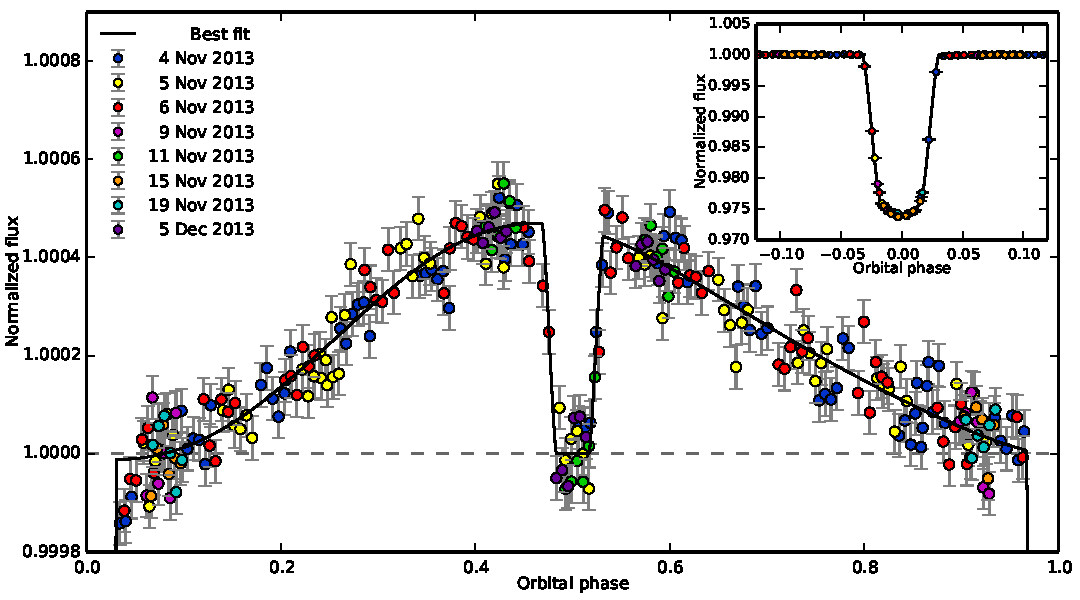
\includegraphics[width=0.5\linewidth]{figures/introduction/stevenson_phasecurve2014.pdf}
    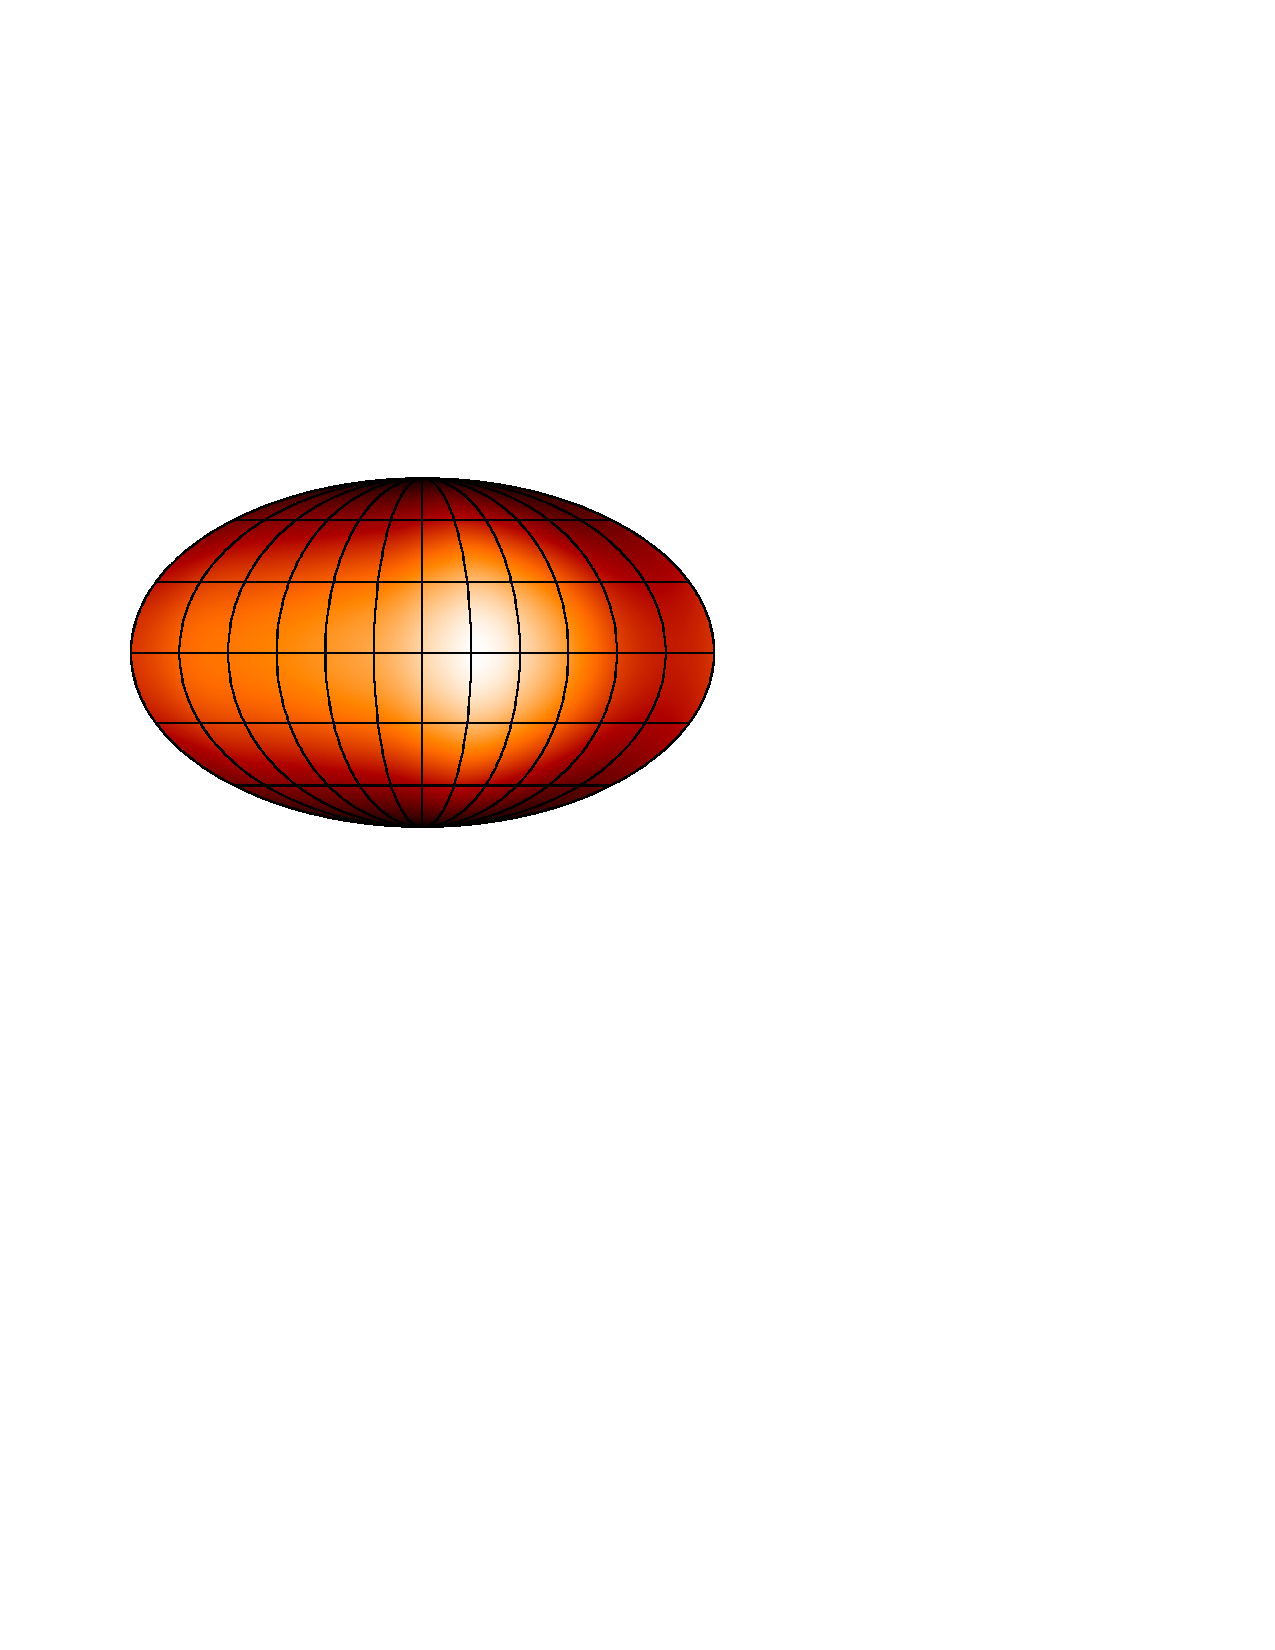
\includegraphics[width=0.4\linewidth]{figures/introduction/knutson_2007_temperature_map_HD_189733b.pdf}
    \caption[Exoplanet phase variations and temperature map.]{Left: Band integrated phase variation of {WASP-43b} from the HST~\citep{stevenson_thermal_2014}.
        The primary transit is inset top right.
        The peak of brightness occurs before the secondary transit.
        Right: Global temperature map of the hot Jupiter HD\,189733b obtained with {Spitzer Space Telescope}~\citep{knutson_map_2007}.
        The hottest point is offset from the sub-stellar point with the day side and night side temperatures around 930\K{} and 650\K{} respectively.}
    \label{fig:phasecurve2014_and_temp_map}
\end{figure}

Secondary transit and phase variations are an extension of the transit method, requiring higher precision to detect the reflection and thermal emission of the exoplanet.
The observed light curve is analysed considering it has two components, not only light from the star but also light from the planet, albeit at a much lower flux level.
To help visualize and discuss the components of exoplanet atmospheres \cref{fig:transits_and_occultations} is provided showing a transiting planet in orbit around a star, in which the planet also passes behind the star causing an occultation.
The planet is shown at several positions of the orbit indicating the proportion of day side and night side observed.
Below the star and planet is a diagram showing the changing flux variation (solid black line) over time, following the orbit.
If the orbital alignment is such that the planet will pass behind the star it will cause an occultation of the planet.
At this point the only light received is from the star alone, creating a baseline stellar measurement.
While during the primary transit there is also a small thermal emission contribution from the night side of the planet, as well as it partially blocking the star.

Throughout the orbit of the planet there is a variation in the planetary flux due to the alternating day/night side of the planet observed.
There are multiple components of the planetary flux, reflection and emission, that can be analysed with multi-band phase curves~\citep[e.g.][]{knutson_characterizing_2009, esteves_optical_2013}.
Optical phase curves will mostly show the reflected light from the day side of the planet, allowing modelling of the atmospheric albedo (fraction of light reflected by the atmosphere), and can provide details on the atmospheric scattering~\citep{madhusudhan_analytic_2012} and aerosol composition~\citep{oreshenko_optical_2016} through the optical phase function (day/night fraction).
Thermal emission of the planet will provide stronger modulation of infrared phase curves and can provide insights into the atmospheres thermal
structure and heat circulation~\citep{goodman_thermodynamics_2009, koll_temperature_2016}.

An example of phase variations in the infrared spectra of {WASP-43b} obtained with the Hubble Space telescope is given in \cref{fig:phasecurve2014_and_temp_map} (left).
The large amplitude of phase variation between the day and night side indicates that the night side is much cooler and there is an inefficient heat circularity from the day to night side.
A planet with an efficient day/night heat distribution mechanism would quickly equalize and have smaller phase variation.
One key observable from \cref{fig:phasecurve2014_and_temp_map} is that the peak of the phase variation is offset from the location of the secondary transit.
The hottest part of the atmosphere does not correspond to the sub-stellar point i.e.\ the point of the planet's surface closest to the star.
This is also observed in surface temperature mapping of the hot Jupiter HD\,189733b obtained with the {Spitzer Space Telescope}~\citep{knutson_map_2007} shown in the right of \cref{fig:phasecurve2014_and_temp_map}.
Simulations of atmospheric circulation models find that this offset is caused by super-rotating equatorial jets which move the location of the hottest point of the planet~\citep[e.g.][and references therein]{heng_atmospheric_2015}.

The point of occultation, at which the planet is completely blocked by the star, enables a baseline measurements for the star to be obtained without the planet.
\textbf{The depth of the occultation, is a direct measurement of the planet-to-star ratio between the star and the planet a }\todo{cite secondary eclipse of reflectance, and secondary spectroscopy examples}.
Spectra obtained during the occultation will have no planetary signal and can be used remove the stellar component from spectra obtained at other phases to obtain the planetary spectrum.


The depth of the occultation is a measure of the flux from the day side of the planet which can indicate the atmospheric reflection and thermal emission of the planet's atmosphere.


\subsection{Transmission spectroscopy}
\label{subsec:transmission_spectroscopy}
\begin{figure}
    \centering
    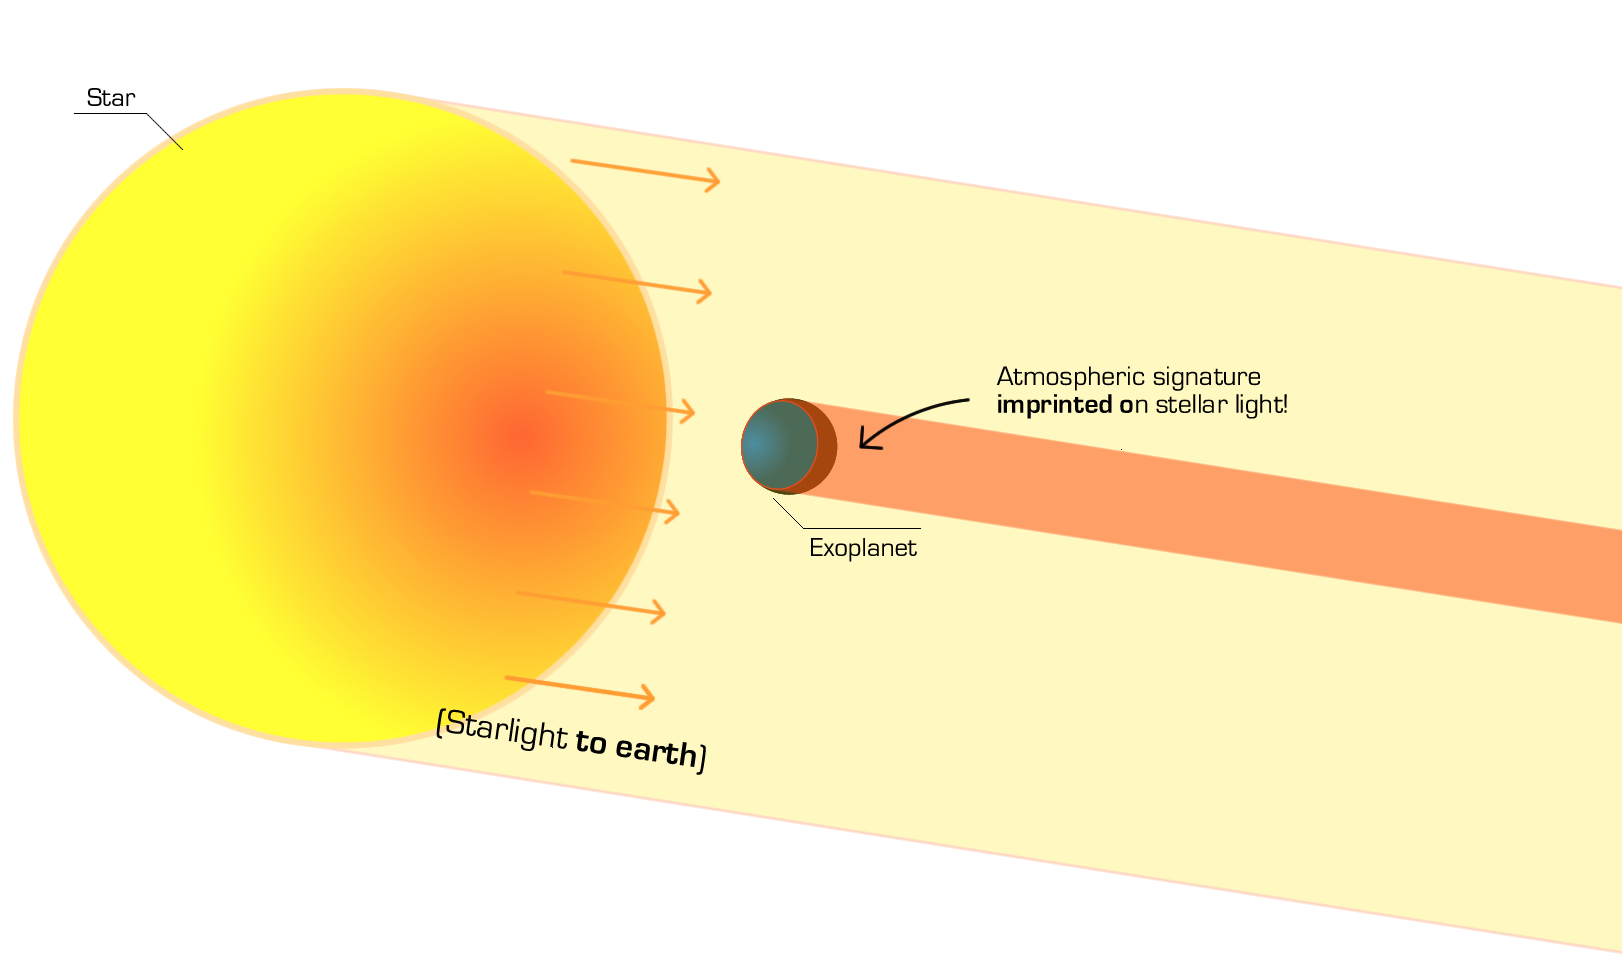
\includegraphics[width=0.65\linewidth]{figures/introduction/transmission_spectroscopy}
    \caption[Transmission spectroscopy diagram.]{Diagram of transmission spectroscopy imprinting the atmosphere of the exoplanet.
        Sourced from \href{http://www.sc.eso.org/~esedagha/research.html}{http://www.sc.eso.org/~esedagha/research.html}}
    \label{fig:transmissionspectroscopy}
\end{figure}

\begin{figure}
    \centering
    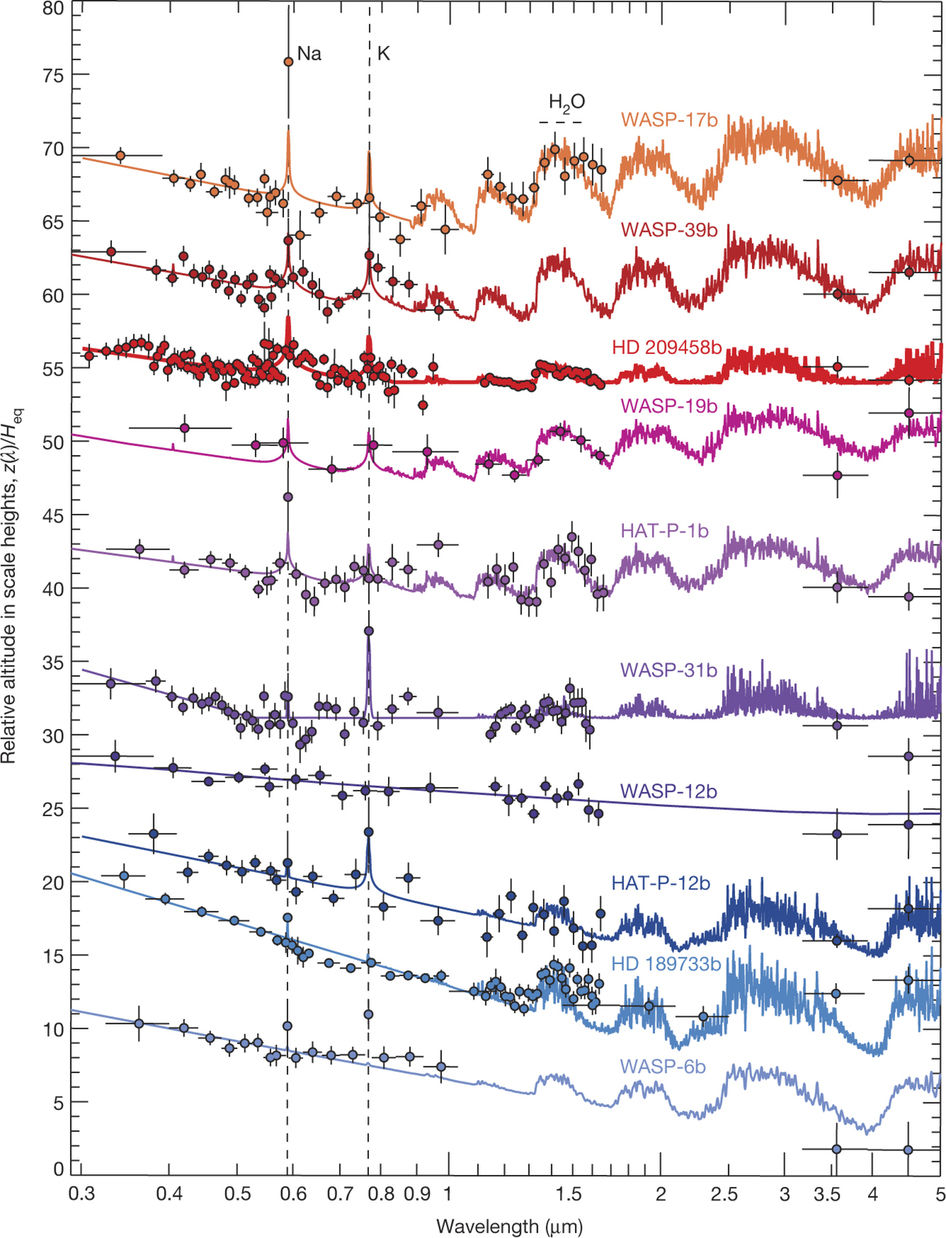
\includegraphics[width=0.6\linewidth]{figures/introduction/transmissionSpec_Sing2016}
    \caption[Transmission spectra for several Hot-Jupiter exoplanets.]{Transmission spectra (dots) for several Hot-Jupiter type exoplanets which increase in the amount of haze and clouds from top to bottom.
        The solid lines indicate the best fit atmospheric models.
        Credit~\citet{sing_continuum_2016}.}
    \label{fig:transmissionspecsing2016}
\end{figure}

When a transiting planet crosses in front of the host star it blocks out light from the star.
However, a small portion of light passes through the atmosphere of the planet as shown in \cref{fig:transmissionspectroscopy}.
The light that passes through the exoplanet atmosphere is partially absorbed, and is faintly imprinted with absorption lines.


In planetary transits, usually defined by their duration and depth, there are degeneracies in the transit shape from a single band, such as the \(\frac{\Rp}{\Rstar}\) ratio.
Observing transits in multiple bandpasses (i.e.\ by splitting the spectra observed during transits into several bands)  has been shown to break the degeneracies between the stellar radius and the orbital inclination as well as determine the stellar limb darkening~\citep{jha_multicolor_2000, knutson_using_2007}.

The radius of the transiting exoplanet can also appear to change size when observed at wavelengths where there is strong opacity in the atmosphere~\citep[e.g.][]{burrows_radii_2000, seager_theoretical_2000}.
Transits in different wavelength bands will have varying depths, dependant on the opacity of the atmosphere to each band. 

The transmission spectra observed with space observatories and ground based high resolution spectrographs have been able to detect several elements and molecules in the atmosphere.
For example \ce{Na}~\citep{charbonneau_detection_2002, redfield_sodium_2008, wyttenbach_spectrally_2015, nikolov_vlt_2016} \ce{H2O}~\citep{tinetti_water_2007, brogi_carbon_2014} \ce{CO}~\citep{brogi_carbon_2014, snellen_mass_2018}, \ce{CH4}~\citep{redfield_extrasolar_2010}, \ce{Fe} and \ce{Ti}~\citep{hoeijmakers_atomic_2018}.
The presence of clouds in the atmosphere have also been detected, as they mask the atmospheric constituents as they produce wavelength-independent fluxes~\citep[e.g.][]{barman_clouds_2011, kreidberg_clouds_2014, sing_continuum_2016}.

Transmission spectra for several transiting Hot-Jupiter exoplanets from~\citet{sing_continuum_2016} is shown in \cref{fig:transmissionspecsing2016}.
The amount of haze and clouds present in the atmospheres increases from top to bottom.
The clearer atmospheres near the top have large alkali lines (\ce{Na} and \ce{K}) and \ce{H2O}, while the cloudier planets lower down have strong optical scattering slopes, narrow alkali lines and partially or completely obscured \ce{H2O} absorption.


\subsection{High resolution spectroscopy}
\label{subsec:high_resolution_spectroscopy}

\begin{figure}
    \centering
    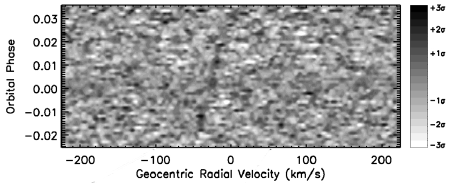
\includegraphics[width=0.7\linewidth]{figures/introduction/snellen2010}
    \caption[Cross-correlation signal from {CRIRES} observations of HD\,209458\,b.]{Cross-correlation signal of {CRIRES} observations during the transit of HD\,209458\,b with a \ce{CO} template.
        Credit~\citet{snellen_orbital_2010}.}
    \label{fig:snellen2010}
\end{figure}

Precise high resolution spectrographs, which are too large and bulky to fly in space, are able to spectrally resolve individual absorption lines, are key for analysing the atmospheres of exoplanets.
The large collecting area of current and future ground based telescopes make high resolution spectroscopy a great contender for obtained high-resolution observations for detecting and exploring exoplanetary atmospheres.

Typically high-resolution and high \snr{} are cross correlated with modelled planetary templates to recover the faint signal of the companion.
This has been most successful in the \nir{} due to the larger planet-to-star flux ratio
notably with CRIRES, with the detection of orbital motion, atmospheric constituents and exoplanetary winds~\citep[e.g.][]{snellen_orbital_2010, dekok_detection_2013, brogi_carbon_2014, brogi_rotation_2016, schwarz_evidence_2015}.
The rotation rate of exoplanets has been achieved by measuring the spectral line broadening~\citep{snellen_fast_2014, brogi_rotation_2016}.
An example of a cross correlated result is given in \cref{fig:snellen2010} showing the shift of the \ce{CO} lines during a transit due to the orbital motion of the planet~\citep{snellen_orbital_2010}.

The spectrum of the star and planet usually cannot be spatially resolved so methods to identify and remove the stellar component are required.
This usually involves constructing a high \snr{} stellar mask from observations, possibly at different phases~\citep[e.g.][]{rodler_weighing_2012}, to subtract from the observed spectra leaving behind the planetary signal.
If the planet is able to be spatially resolved, then a spectrum of the planet could be obtained without stellar contamination~\citep[e.g.][]{snellen_combining_2015}.

High resolution spectroscopy of atmospheres is not limited to transit spectroscopy with detections also possible for non-transiting exoplanets~\citep[e.g.][]{brogi_signature_2012, brogi_carbon_2014,lockwood_nearir_2014, piskorz_evidence_2016}.

An advantage of high-resolution spectra is that it allows the molecular absorption lines of Earth's atmosphere to be resolved.
This way they can be identified and corrected/removed to avoid contamination with the atmosphere of the exoplanet.
 Lower resolution and photometric methods are unable to fully resolve and remove Earth's atmosphere from ground based observations.



%!TEX root = ../../thesis.tex

\section{The diversity of exoplanets}

Exoplanetary detections have challenged the theoretical formation models with their variety and distribution of sizes and, locations.
For instance, the discovery of the hot-Jupiter class (large mass planets on close in orbits) challenged the accepted planet formation theories at the time~\citep[.e.g][]{pollack_formation_1996, boss_giant_1997} in which our Solar System was thought to be typical with small rocky planets close to the Sun and large giant planets further away.

The precise characterization of more exoplanets with the detection of exoplanetary atmospheres will allow for the constraints of exoplanetary composition and formation mechanisms to be improved.
For instance, the core accretion model has been able to reproduce the large number of Super-Earths, the correlation between star metallicity and planet frequency~\citep[e.g.][]{santos_spectroscopic_2004, fischer_planetmetallicity_2005}, and the presence of many Hot-Jupiter and Neptune like planets in close-in orbits, with the help of migration mechanisms~\citep[e.g.][]{triaud_exoplanets_2016}.
Recent models also combine both planetary formation and evolution to describe the observed exoplanets~\citep[e.g.][]{mordasini_characterization_2012} and can reproduce general population properties in a statistically significant way~\citep{mordasini_extrasolar_2009}.

A proxy for the composition and structure of an exoplanet is the average density, computed from the mass and radius.
A mass-radius diagram is shown in \cref{fig:santerne2018} for Earth-like rocky planets.
The tracks show contours of mass-radius for different theoretical compositions~\citep{brugger_constraints_2017}, while the circles indicate a number of detected small mass exoplanets, with {K2-229\,b} being a Super-Earth with a Mercury-like density~\citep{santerne_earthsized_2018}.
The density can give an approximate composition but for a given mass there are an infinite number of combinations of metal/silicate/ice and gas that can produce the same radii~\citep[e.g.][]{seager_massradius_2007}.
Low mass planets tend to be rocky and tend to have small or no atmosphere.
With rock being in-compressible, to first order, it is relatively insensitive to the incident flux.
The radii of solid exoplanets are sensitive to gas content of the atmosphere as a small increase in \ce{H} and/or \ce{He} can cause a large increase in radius~\citep{adams_ocean_2008}.

\begin{figure}
    \centering
    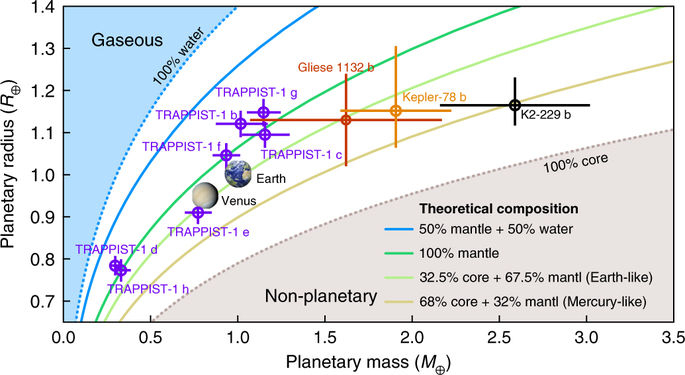
\includegraphics[width=0.7\linewidth]{figures/introduction/santerne_2018}
    \caption[Mass-Radius diagram for rocky planets with composition contours.]{Mass-Radius diagram for rocky planets with composition contours.
        Adapted from~\citet{santerne_earthsized_2018}}
    \label{fig:santerne2018}
\end{figure}

When the gas component becomes dominate, planets begin to have radii independent of their mass~\citep[e.g.][]{lopez_understanding_2014}.
The atmospheres of gas giants are also susceptible to stellar irradiation, with close in Hot-Jupiters having inflated atmospheres and larger radii~\citep[e.g][]{fortney_interior_2010}.


\begin{figure}
    \centering
    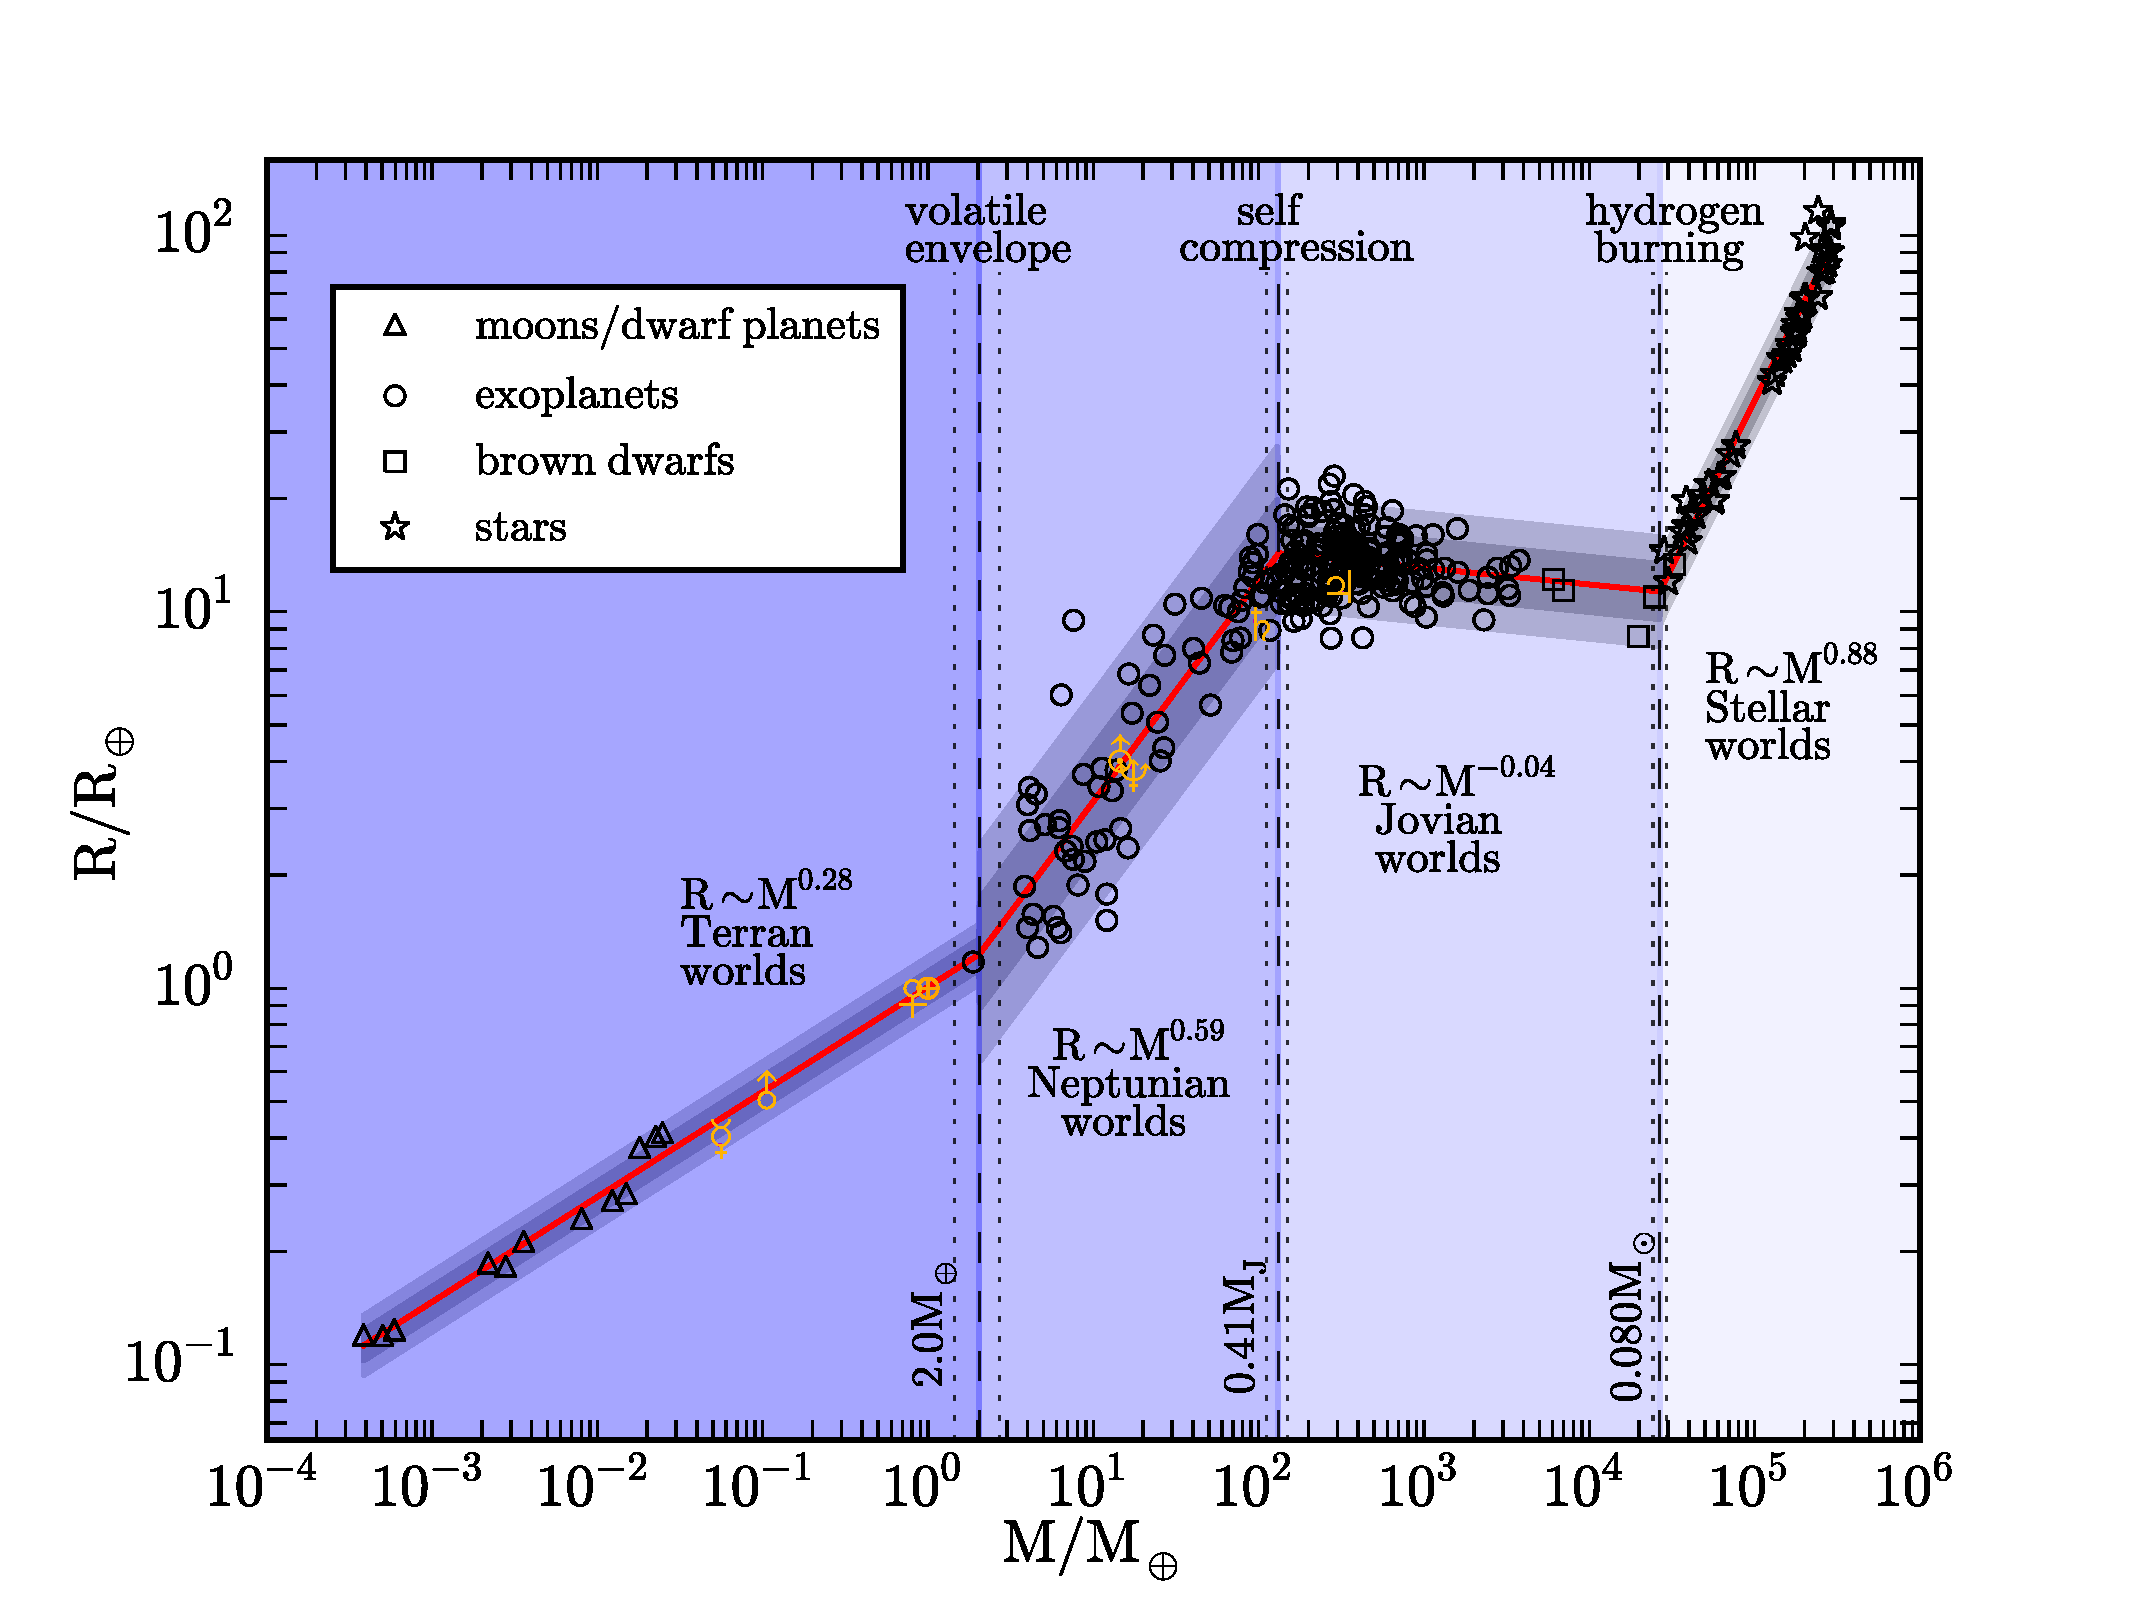
\includegraphics[width=0.7\linewidth]{./figures/introduction/mass_radius_relation.pdf}  \\
    \caption[Mass-Radius relationship with probabilistic fit.]{Mass-Radius relationship with probabilistic fit from dwarf planets to late-type stars from~\citet{chen_probabilistic_2016}.
    The black symbols represents the objects used to fit the model, with the key in the top-left, while the orange symbols represent the solar system planets.
    The red line indicates the average value, while the light and dark grey regions indicate the 65\% and 95\% confidence intervals.}
    \label{fig:mass_radius_relation}
\end{figure}

Models of the mass-radius relation are important as they enable insight into the likely planetary properties when only either mass or radius can or has been measured.
For example~\citet{chen_probabilistic_2016} developed a probabilistic model over 9 orders-of-magnitude in mass and 3 orders-of-magnitude in radius, with the result shown in \cref{fig:mass_radius_relation}.
There are four separate power laws and three different transition regions fitted by the model.
This breaks the mass radius relation into different regions classified after a representative example from our solar system.
The lowest mass range is the rocky "Terran" worlds up to 2.0\,\(\textrm{M}_oplus\) and inclusive of dwarf planets, "Neptunian" worlds between 2.0,\(\textrm{M}_oplus\) and 0.41\,\Mjup{} and, "Jovain" worlds between 0.41\,\Mjup{} and 0.08\Msun{}.
The transitions regions are indicative of a changing composition or physical processes (such as the hydrogen burning limit in stars) and consistent with other works~\citep[e.g.][]{weiss_mass_2013, dieterich_solar_2014, hatzes_definition_2015, rogers_most_2015}.

Recently, there has been a renewed interest in Brown Dwarf (BD) candidates triggered by exoplanetary searches as they bridge the gap between giant planets and low-mass stars.
It is difficult to distinguish between giant planets and BDs with a loosely suggested definition of mass between 13--80\,\Mjup{}\footnote{0.01--0.08\Msun{}} for Brown Dwarfs as this is between the Deuterium fusion mass of around 13\,\Mjup{}~\citep[e.g.][]{spiegel_deuteriumburning_2011} and the Hydrogen fusion limit of 80\,\Mjup{}~\citep{chabrier_theory_2000, dieterich_solar_2014}.
Several works found similar properties on the two populations, like a similar density~\citep{hatzes_definition_2015, chen_probabilistic_2016} seen in \cref{fig:mass_radius_relation} by the same power law spanning giant planets and BDs, while others have found intriguing differences.
When classified using just mass and size~\citet{chen_probabilistic_2016} find no difference between giant planets and Brown Dwarfs, with Brown Dwarfs just being large giant planets.

There is a paucity of {BD} companions in short period orbits around Sun-like stars (\(\lesssim{}5 \)\AU{}), compared to stellar or planetary companions, termed the \emph{brown dwarf desert}~\citep{halbwachs_exploring_2000, zucker_analysis_2001, sahlmann_search_2011, ranc_moa2007blg197_2015} which can been seen as the gap in the "Jovian" worlds section of \cref{fig:mass_radius_relation}.
There are observed differences in the host star metallicity~\citep{maldonado_searching_2017, santos_observational_2017, schlaufman_evidence_2018} and orbital eccentricity distribution~\citep{ma_statistical_2014} either side of the period/mass gap with the lower mass BDs having properties similar to giant planets and high mass BDs having properties more like stars.
There is a very strong hint of different formation mechanisms as BDs below the gap may primarily form via gravitational instability in protoplanetary disks, while above this gap BDs may form more like stellar binary from molecular cloud fragmentation~\citep{ma_statistical_2014}.

As the number of known BDs orbiting solar type stars is low, the characterization of benchmark BDs in the brown dwarf desert~\citep[e.g.][]{crepp_trends_2016} is beneficial in understanding this sub-stellar population and to help constrain formation and evolution theories~\citep{whitworth_formation_2007}.
There is an inherent degeneracy between the mass, age and luminosity of a given BD~\citep{burrows_nongray_1997} because without sustained fusion, BDs cool down over time with an age-dependent cooling rate.

BDs in binary systems, unlike free-floating BDs~\citep[e.g][]{gagne_simp_2017}, allow for the determination of their masses, when complemented with radial velocity ({RV}) and astrometry measurements.
The {RV} technique provides the mass lower-limit (\Mtwosini{}) of binary and planetary companions, while complementary astrometry measurements can often provide mass upper-limits~\citep[e.g.][]{sahlmann_search_2011}.
Measuring or tightening the constraints of {BD} masses improves the understanding of mass dependence on {BD} formation processes.
Photometry along with stellar evolution models~\citep[e.g.][]{baraffe_evolutionary_2003,allard_btsettl_2013} can also be used to estimate the mass of {BD} companions~\citep[e.g.][]{moutou_eccentricity_2017} if there is sufficient orbital separation, and a precise determination of the age~\citep{soderblom_ages_2010}.


%
%\begin{figure}[t]
%    \centering
%    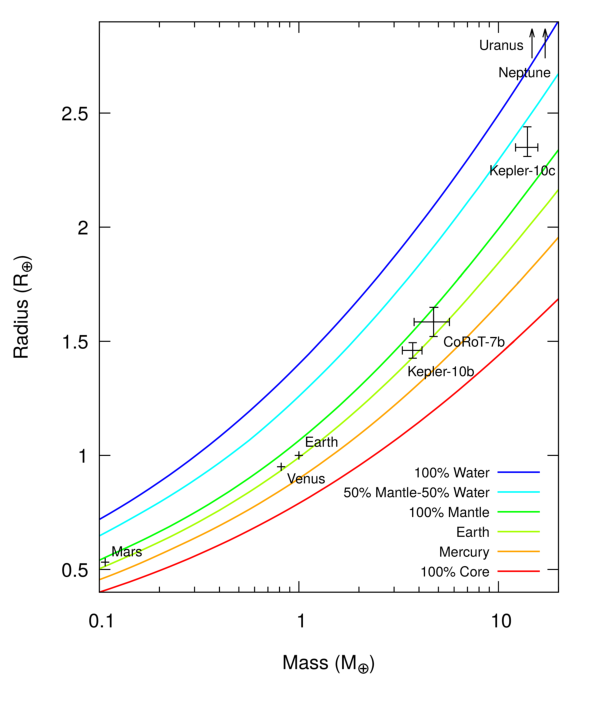
\includegraphics[width=0.4\linewidth]{./figures/introduction/Mass_radius_relation-compostion_Brugger_2017.pdf}
%    \caption[]{Mass-Radius relationship for (super) Earth-like planets with composition contours.
%        Adapted from~\citet{brugger_constraints_2017}}
%    \label{fig:mass_radius_relation_composition}
%\end{figure}
%
%
%
%\begin{figure}
%    \centering
%    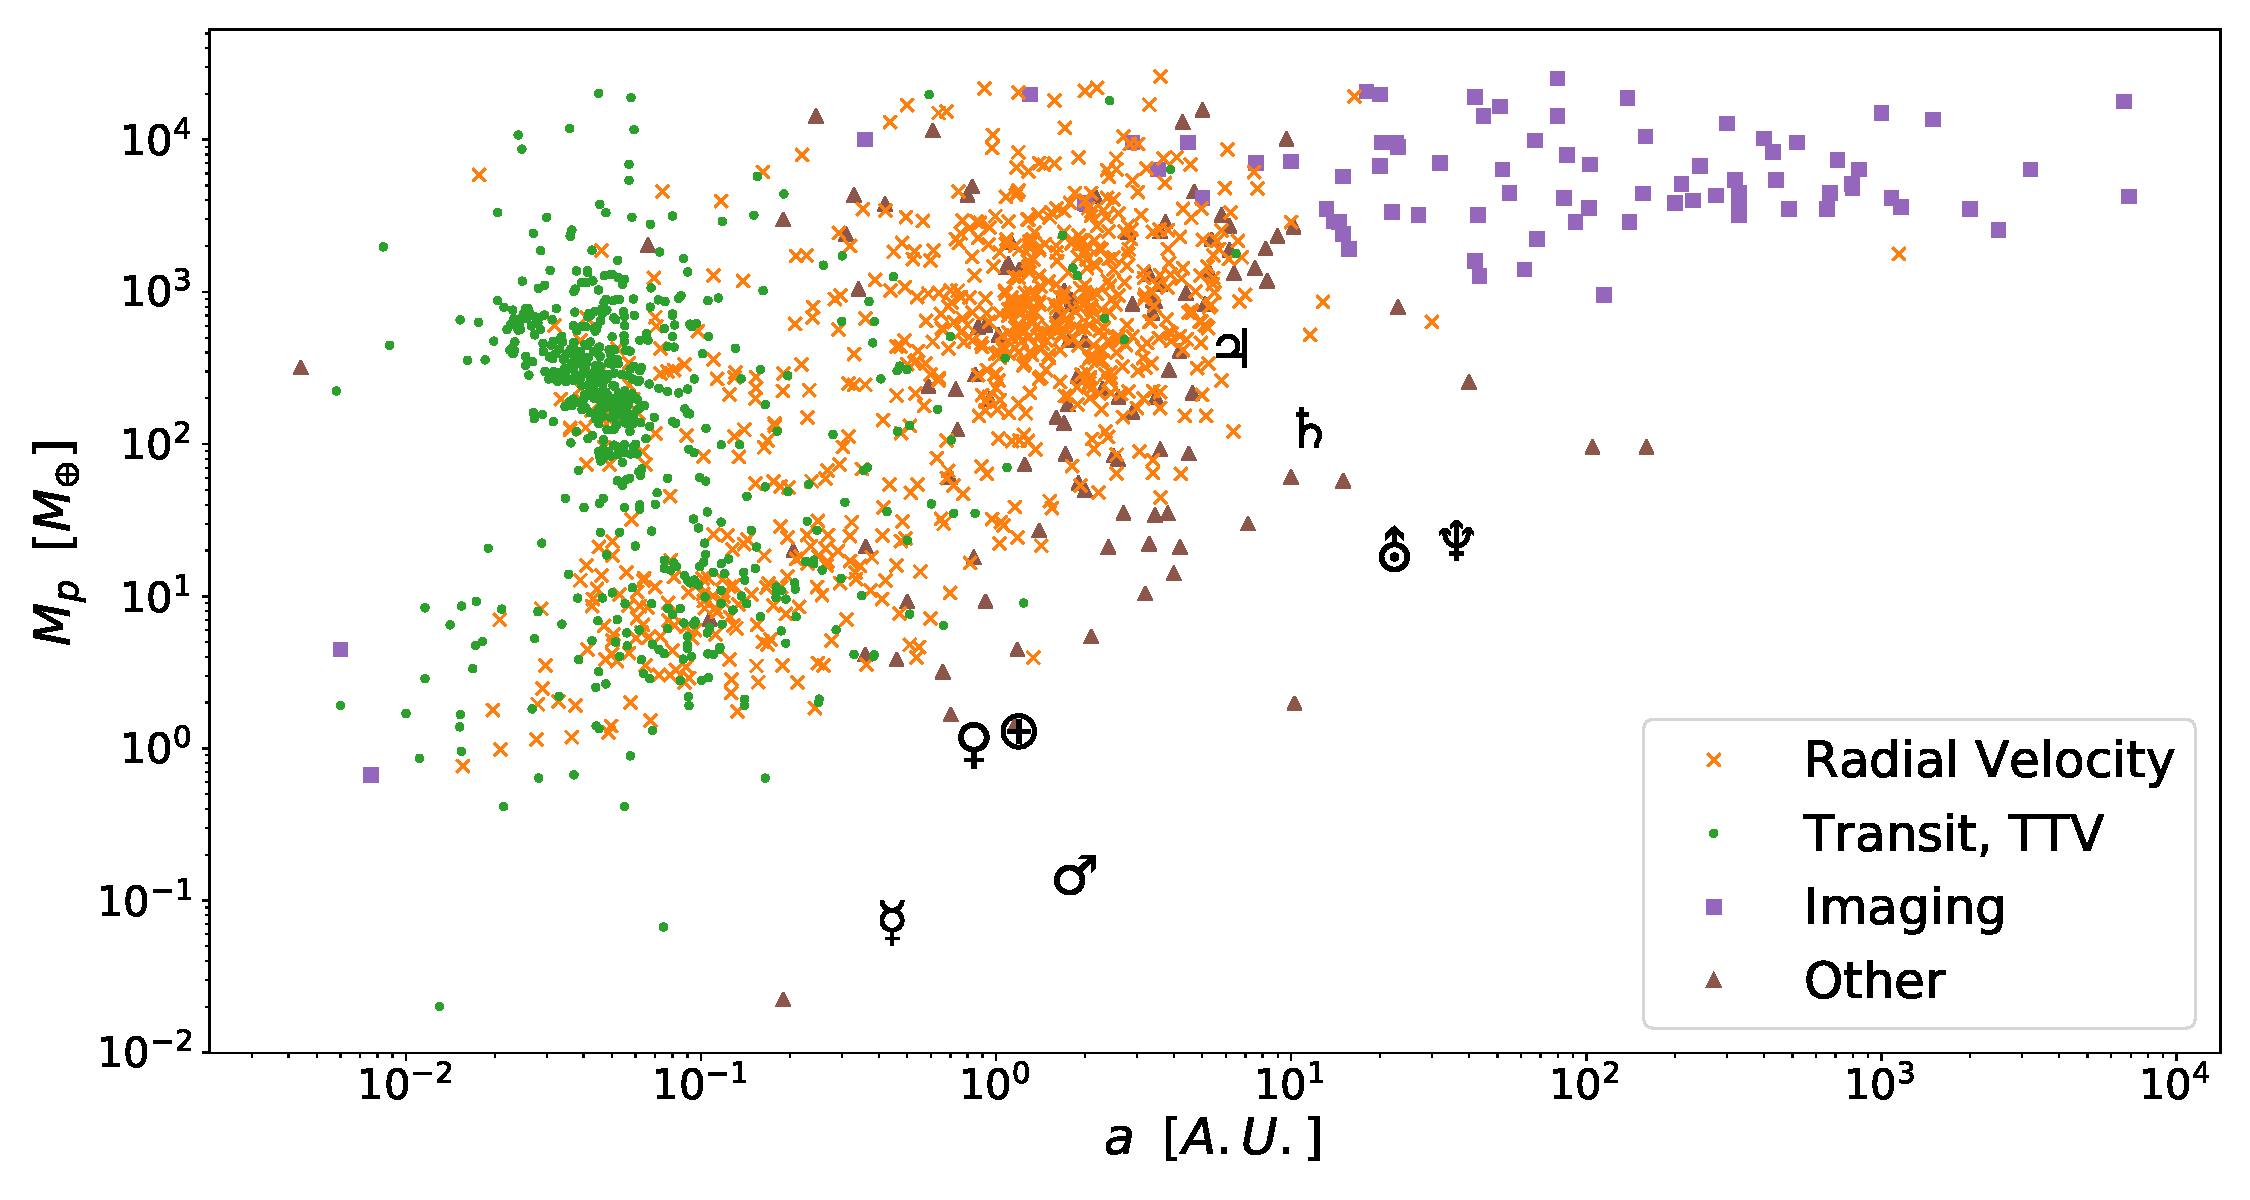
\includegraphics[width=0.\linewidth]{./figures/introduction/exoplanetEU_a_mass.pdf}
%    \caption[]{Exoplanet semi-major axis verses mass diagram.
%        The symbols indicate the location of the solar system planets, $\mercury$-Mercury, $\venus$-Venus, $\earth$-Earth, $\mars$-Mars, $\jupiter$-Jupiter, $\saturn$-Saturn, $\uranus$-Uranus, $\neptune$-Neptune.
%        Data from \href{http://ww.exoplanet.eu}{exoplanet.eu} October 2018}
%    \label{fig:pltoverlayadd}
%\end{figure}
%
%
%Explore what these method have found with exoplanet populations.









\section{Paper Introduction}\label{sec:intro}
Brown dwarfs (BDs) are sub-stellar objects unable to achieve hydrogen fusion, with masses around \(13-80~\textrm{M}_{jup} \)~\citep{chabrier_theory_2000}, bridging the gap between low-mass stars and giant planets.
Without sustained fusion, brown-dwarfs cool down over time with an age-dependent cooling rate.
Therefore, there is an inherent degeneracy between the mass, age and luminosity of a given BD~\citep{burrows_nongray_1997}.
This degeneracy may be resolved by the observation of several parameters, for instance when a BD is in a binary system with a main sequence host star, using both the host stars age and the masses derived from the dynamical motion.

A paucity of BD companions exists in short period orbits around Sun-like stars (\(\lesssim5 \)\AU), compared to stellar or planetary companions, termed the \emph{brown dwarf desert}~\citep{halbwachs_exploring_2000, zucker_analysis_2001, sahlmann_search_2011}.
As the number of known BDs orbiting solar type stars is low, the characterization of benchmark BDs in the brown dwarf desert~\citep[e.g.][]{crepp_trends_2016} is beneficial in understanding this sub-stellar population and to help constrain formation and evolution theories~\citep{whitworth_formation_2007}.
The BD desert also provides a greater challenge as it reduces the amount of good BD candidates to study.

BDs in binary systems, unlike free-floating BDs, allow for the determination of their masses, when complemented with radial velocity ({RV}) and astrometry measurements.
The {RV} technique provides the mass lower-limit (\mtwosini{}) of binary and planetary companions, while complementary astrometry measurements can often provide mass upper-limits~\citep[e.g.][]{sahlmann_search_2011}.
Measuring or tightening the constraints of BD masses improves the understanding of mass dependence on BD formation processes.
For instance, there is growing evidence that the larger giant planets and BD companions do not follow the well known metallicity-giant planet correlation seen in main-sequence stars with planets~\citep[e.g.][]{santos_spectroscopic_2004,santos_observational_2017, maldonado_searching_2017}.
Photometry along with stellar evolution models~\citep[e.g.][]{baraffe_evolutionary_2003,allard_btsettl_2013} can also be used to estimate the mass of BD companions~\citep[e.g.][]{moutou_eccentricity_2017} if there is sufficient orbital separation, and a precise determination of the age~\citep{soderblom_ages_2010}.

Recently, there has been a renewed interest in BD candidates triggered by exoplanetary searches.
While several works found similar properties on the two populations, like a similar density~\citep{hatzes_definition_2015}, others found intriguing differences.
One of the most recent is the different host metallicity of the Brown Dwarf and giant planet populations~\citep{santos_observational_2017, schlaufman_evidence_2018}, a very strong hint of different formation mechanisms.

Spectral observations of binary systems contain the spectra of both bodies, in proportion to their flux ratio, and Doppler shifted relative to each other due to their orbital motion.
One technique to recover the spectra of the companion is secondary reconstruction through a differential spectrum~\citep{ferluga_separating_1997}.
Spectra from different phases are shifted to the rest frame of the host star and subtracted to mutually cancel out the spectrum of the host star allowing the faint companion spectra to become visible.
Advances in high-resolution and near-infrared (\nir{}) capabilities should enable this technique to be applied to BDs and planet companions, in which smaller {RV} shifts can be resolved and the contrast ratio of the smaller companion is improved.

Observing in the \nir{} is specifically desirable for the cooler sub-stellar and giant planet companions as their thermal emission is stronger in the infrared compared to the optical.
This improves the contrast ratio between the host star and companion, providing favourable conditions for their detection and spectral separation.
CRIRES, a high resolution \nir{} spectrograph, has made many prominent advances in recent years with the detection of atmospheric constituents, such as \(\textrm{CO} \) and \(\textrm{H}_{2}\textrm{O} \), atmospheric winds and thermal profiles, rotation and orbital motion, for both transiting and non-transiting planets~\citep[e.g.][]{snellen_orbital_2010, brogi_signature_2012, rodler_weighing_2012, dekok_detection_2013, brogi_carbon_2014, snellen_fast_2014, piskorz_evidence_2016, brogi_rotation_2016, birkby_discovery_2017}.

The higher temperature and relatively larger size of BDs compared to giant-planets makes the development of spectral recovery techniques for BD companions a logical step towards the spectroscopic detection of planetary atmospheres.
There has been the recent installation and continued development of many new high-resolution \nir{} spectrographs, such as {CARMENES}~\citep{quirrenbach_carmenes_2014}, NIRPS~\citep{bouchy_nearinfrared_2017} or SPIRou~\citep{artigau_spirou_2014}, as well as, the {CRIRES+}~\citep{dorn_crires_2016} upgrade.
These new instruments motivate the study of \nir{}-oriented methodologies for spectral recovery, and are of high importance due to the larger planet-to-star flux ratio provided by near-IR compared to the visible.

{\rd{} The search and detection of faint secondary spectra is not only relevant to planetary atmospheres.
\citet{kolbl_detection_2015} developed a method to detect the presence of optical secondary spectra down to a flux ratio of 1\% in the hosts of \emph{Kepler} transit candidates.
The presence of which can cause ambiguities in the system configuration, and increase the uncertainty of the measured planet radius.
The characterization of the false positive probability rate for Kepler has been found to be as high as \(\sim\)35\%~\citet{santerne_sophie_2012}.}

In this paper we apply two different techniques on FGK stars with BD companions with the aim to spectroscopically detect their companions.
In \sref{sec:data} we present the observations and reduction process as well as the spectral models used in this work.
In \sref{sec:specdiff} we explain the differential spectral technique and its applicability to these observations while in \sref{sec:results} we apply companion recovery using a \textchisquared{} approach.
In \sref{sec:discussion} we discuss our results and in \sref{sec:conclusions} we present our conclusions.



brown dwarf dessert explore \citet{ranc_moa2007blg197_2015}

%!TEX root = ../../thesis.tex
\clearpage
% Motivation of this work
\section{Motivation}
\label{sec:motivation}

As shown in this introduction there is a vast field of exoplanet research, with one of the current challenges being the detection of planetary atmospheres, in the near infrared specifically. The purpose of this thesis is to develop methodologies and tools to extract he minute signals of planetary spectra from \nir{} spectra. Having access to \nir{} CRIRES spectra of stars with suspected Brown Dwarf companions\footnote{Only the minimum mass \mtwosini known} it was decide that this would be an excellent starting point to develop the techniques to recover the secondary spectrum. For one, the Brown dwarf companion spectra should have a higher flux ratio than an exoplanet, and hence be easier to detect, and secondly, being able to recover the spectra of these companions would help to constrain the mass of the companions, differentiating them from low-mass stars, and helping to complete the puzzle regarding BD companions.

This would be used a stepping stone to request observational time and apply the techniques on giant exoplanets in the \nir{} with the state of the art detectors that are being developed.  

The fundamental concepts of \nir{} spectroscopy, the radial velocity method, and synthetic models are provided in \cref{cha:concepts}. The process of reducing \nir{} CRIRES spectra, with a comparison between two different reduction software is given in \cref{cha:reduction}, followed by the post reduction calibration and atmosphere correction required.

\cref{cha:direct_recovery} presents spectral disentanglement techniques, focusing on the application of a differential subtraction technique to the \nir{} spectra of Brown Dwarf companions. A second technique is developed in \cref{cha:model_comparison} which attempts fitting the observations with two synthetic spectral components.

Towards a slightly different goal, \cref{cha:nir_content} contains work computing the fundamental RV precision of {M-dwarf}in the \nir{}. These are the best candidates for detecting small mass planets in their habitable zone, and are a focus for upcoming \nir{} RV spectrographs. Understanding the fundamental precision attainable from the models and observed spectra.\todo{I am just making this up at the moment}{ will help understand the precision and detectability of low-mass planets???}. Focus was shifted towards updated the tools to compute the RV precision to prepare for the release of the CARMENES \nir{} spectral library.


    %!TEX root = ../thesis.tex
%2 - Tools for spectral analysis

\chapter{Advanced Concepts}
\label{cha:concepts}
To put things too detailed for the introduction?
    %!TEX root = ../thesis.tex
%2-Tools for spectral analysis
% Reduction processes for NIR
% Additions to IRAF toolchain
% Problem with order tracing
%
% Wavelength Calibration
%    All detectors together
%    With stellar and ThAr lines???
% Telluric Correction


\chapter{Tools for spectral analysis}  % Main chapter title
\label{cha:reduction} 

%----------------------------------------------------------------------------------------
%	SECTION 1
%----------------------------------------------------------------------------------------

\section{Main Section 1}



%-----------------------------------
%	SUBSECTION 1
%-----------------------------------
\subsection{Subsection 1}


%-----------------------------------
%	SUBSECTION 2
%-----------------------------------

\subsection{Subsection 2}
Useful information about MIR reduction in VISIR manual
\href{https://www.eso.org/sci/facilities/paranal/instruments/visir/doc/VLT-MAN-ESO-14300-3514_2018-02-01.pdf}{https://www.eso.org/sci/facilities/paranal/instruments/visir/doc/VLT-MAN-ESO-14300-3514_2018-02-01.pdf}
%----------------------------------------------------------------------------------------
%	SECTION 2
%----------------------------------------------------------------------------------------

\section{Main Section 2}




	%!TEX root = ../thesis.tex
%3-Direct-Spectral-Recovery
% Shift and subtract Method
% Calculation of planet {RV}
% Simulation of spectral recovery
% {RV} difference effect on amplitude of signal simulation
% Chi squared method of model plus stellar at different RVs? technique
% Limitations?
% Future Prospects
% {CRIRES+}, JWST
% Calculation of exposure time required etc?


\chapter{Direct Spectral Recovery}  % Main chapter title
\label{cha:direct_recovery}
%----------------------------------------------------------------------------------------
%    SECTION 1
%----------------------------------------------------------------------------------------
There many different techniques to disentangle the spectra of binary objects. In this chapter we focus on applying a direct subtraction method to near-infrared (\nir{}) spectra of FGK stars with Brown Dwarf (BD) companions. The data used was obtained with the {CRIRES} instrument in 2012, (before it was removed its upgrade) with the purpose to apply this technique specifically. A level of trust was placed in the quality of the observations, which was misplaced.
We start this chapter by explaining the direct subtraction technique. We will then explain the motivation for the specific targets observed. We will detail the observations, showing each the orbital position of each observation. After revealing the insufficient signal from this technique we will explore the limitations of these observations followed by some simulated results.

\section{Motivation}


Motivation section

Why this technique and not others.
- separation of components
- direct imaging (cant separate)


Find direct imaging limitations ---



\section{Differential subtraction (new)}
\label{sec:spec_diff}
{\red{} This is the summary in the paper}
The observations were gathered having in mind the application of a differential subtraction method~\citep[e.g.,][]{ferluga_separating_1997, kostogryz_spectral_2013} to detect the spectra of the faint BD companions. In short, we Doppler shift each observation to the rest frame of the host star and then mutually subtract the spectra from pairs of observations to cancel out the spectra of the brighter host star. The residuals from this method should contain two copies of the faint companion, subtracted from each other with a radial velocity offset \(\Delta {RV}\) between them. This {RV} offset, if detectable, would allow the mass ratio to be determined and hence the companion mass.

Due to the poorly separated observation times relative to the long orbital periods, this method was revealed to be inappropriate for these observations as the {RV} separation of the companion spectra between observations (\(\le 2.3\)\kmps{}) is significantly smaller than the {FWHM} (full width half maximum) of individual spectral lines (\(\sim\)6\kmps{} at \(\rm R=50\,000\)).  The small separation of the companion causes the lines of the companion to also mutually cancel, severely reducing the residual signal to well below the available noise level. The requirement of well separated RVs for the companion spectra was clearly stated in the original proposal but was not satisfied when the observations were obtained\footnote{see \sref{subsubsec:differential-schedualing} for more details}. {\red{} The very large orbital periods of some of the targets would not produce a sufficient {RV} signal during one semester. This was a possible oversight during the proposal stage.} The largest estimated companion \(\Delta {RV}\) separation between the observations of each target is provided in the seventh column of \tref{tab:estimated_rv}. Radial velocity constraints are also valid for other studies such as the detection of reflected light from exoplanets~\cite{martins_evidence_2015}.

{\red{} Despite these problems, we still tried to apply the method to our data. Given the negative result, however, we decided to move this section to Appendix~\ref{sec:direct-subtraction}, where we describe the method and some exploratory results that may be useful for future studies.
}


\section{Direct Subtraction Method}
\label{sec:direct-subtraction}
Here we outline the direct subtraction method used, which is similar to previous works~\citep{ferluga_separating_1997,kostogryz_spectral_2013}. Assuming that the instrumental profile and atmospheric absorption are dealt with appropriately, the spectrum received from the host-companion pair is given by the superposition of two spectral components (\(J_{1}\), \(J_{2}\)), where \(\lambda-v\) represents the Doppler shift \(\lambda(1-v/c)\) by velocity \(v\).
\begin{equation}
\textrm{I}(\lambda) = \textrm{J}_{1}(\lambda - v_{1}) + \textrm{J}_{2}(\lambda - v_{2})
\end{equation}
or shifted to the host stars rest frame,
\begin{equation}
\textrm{I}(\lambda + v_{1}) = \textrm{J}_{1}(\lambda) + \textrm{J}_{2}(\lambda - v_{2} + v_{1})
\end{equation}
Here, the subscripts 1 and 2 indicate the spectrum of the host and companion respectively, and \(\lambda\) represents the wavelength of the spectra.
The spectra of the host star (\(\textrm{J}_{1}\)) is removed though the mutual subtraction of the host spectrum from two separate observations, denoted with subscripts \(a\) and \(b\), correcting for {RV} motion of the host star.
\begin{align}
S(\lambda) &= \textrm{I}_{a}(\lambda + v_{1a}) - \textrm{I}_{b}(\lambda + v_{1b}) \nonumber \\
&= \textrm{J}_{2}(\lambda - v_{2a} + v_{1a}) - \textrm{J}_{2}(\lambda - v_{2b}  + v_{1b}) \nonumber \\
%  &= \textrm{J}_{2}(\lambda - v_{2a}) - \textrm{J}_{2}(\lambda - v_{2b} - v_{1a} + v_{1b}) \nonumber \\
S(\lambda + v_{2a}) &= \textrm{J}_{2}(\lambda) - \textrm{J}_{2}(\lambda + \Delta {RV}) \label{eqn:sprofile}
\end{align}
where,
\begin{equation}
\Delta {RV} = v_{2a} - v_{2b} - v_{1a} + v_{1b} \label{eqn:k}
\end{equation}

is the actual {RV} difference (\(\Delta {RV}\)) between the two companion spectra.

The resulting differential spectra, dubbed \emph{s-profile} by~\citet{ferluga_separating_1997}, is composed of just the companion spectra, shifted and subtracted from itself.

From binary dynamics~\citep[e.g.,][]{murray_keplerian_2010} the {RV} amplitudes of the host and companion are related through the mass ratio, \(q\), while having an opposite sign.
\begin{align}
v_{2}  &= -\textrm{q} * v_{1} \label{eqn:q_relation}
\end{align}
This equation was used to calculate the expected companion {RV} for each observation in \tref{tab:observations}.

We can simplify \eref{eqn:k} by expressing it in terms of the host {RV} and mass ratio,
\begin{align}
k &= -q v_{1a} + q v_{1b} + v_{1a} - v_{1b} \nonumber \\
&= (1 - \textrm{q})(v_{1a} - v_{1b}). \label{eqn:k_simplified}
\end{align}
If we are able to determine the \(\Delta {RV}\) between the the companion spectra, k, from the s-profile~\citep[see][]{ferluga_separating_1997} then we can determine the mass ratio of the system, q, thereby constraining the mass of the companion. The values \(v_{1a}\) and \(v_{1b}\) are calculated from the orbital parameters of the system and are the same values already used to shift and mutually cancel the host spectrum.

This method is very similar to~\citet{kostogryz_spectral_2013} except that they focus on M-dwarfs host stars with the observations taken at the extrema, in which the companion lines are well separated.




\subsection{The Data}

\subsection{CRIRES data}
\label{subsec:CRIRES}
Observations were performed with the {CRIRES} instrument~\citep{kaeufl_crires_2004} configured to observe a narrow wavelength domain of the \emph{K}-band between 2\,120--2\,160\nm{} using the Ks and the Hx5e-2 filters. The slit width of \(0.4\sec\) resulted in an instrumental resolving power of \(\rm R=50\,000\), with no adaptive optics to ensure that the slit was entirely covered by each target. This prevents strong slit illumination variations that could change the shape of spectral lines.

The observations were performed in service mode during period 89 with run ID.~089.C-0977(A) between April and August 2012. An observation is composed of 8 individual spectra with an integration time of 180 seconds, observed in the ABBAABBA nod cycle pattern to obtain a high (>100) signal-to-noise when combined. The list of observations obtained with {CRIRES} are provided in \tref{tab:observations}.

%!TEX root = ../nir_companions.tex

% Table of observations
\begin{table*}
    \small
            \centering  
           \begin{threeparttable}[b]
     
            \caption{Details about the each CRIRES observation. {\rd{} The time, settings, number of artefacts removed, the SNR obtained and the predicted orbital state of each system are provided.}}
            %\begin{tabular}{l c c c c cl cl r@{.}l r@{.}l r@{.}l}
            \begin{tabular}{l c c c c c c r@{.}l r@{.}l r@{.}l}
                \toprule
                Object & Obs. \# & Start date  & Filter & Airmass  & Artefacts & SNR & \multicolumn{2}{c}{\(RV_1\)} & \multicolumn{2}{c}{\(RV_2\)} & \multicolumn{2}{c}{\(rv_2\)}  \\  % & \(Date \)
                &   & (yyyy-mm-dd hh:mm:ss)  &  & (at start) & {\rd / 32} & & \multicolumn{2}{c}{kms\(^{-1}\)} & \multicolumn{2}{c}{kms\(^{-1}\)} & \multicolumn{2}{c}{kms\(^{-1}\)}\\ % data ref    % & (JD\(^{\star} \))
                \midrule
                {HD 4747}   & 1 & 2012-07-06 07:36:06 & Ks     	      & 1.25  	  & 7 & 340 & $-$0    & 219 & $-$0  & 154 & 0&065 \\ %-1      & 2456114.81674
                {HD 162020} & 1 & 2012-07-04 06:23:22 & Ks     		& 1.30 		& 2 & 127 & $-$28  & 760 & 50 & 785\tnote{a}  & 79&545\tnote{a} \\ %-1      & 2456112.76624
                {HD 162020} & 2 & 2012-07-04 06:57:48 & Ks     		& 1.44  	& 2 & 128 & $-$28  & 717 & 48 & 440\tnote{a} & 77&157\tnote{a} \\ %-2      & 2456112.79015
                {HD 167665} & 1 & 2012-07-28 05:00:53 & Hx5e-2 	& 1.24 		& 7 & 371 & 7         & 581 & 18 & 024\tnote{a} & 10&443\tnote{a} \\ %-1a     & 2456136.70895
                {HD 167665} & 2 & 2012-07-28 05:37:27 & Hx5e-2 	& 1.39  	& 4 & 374 & 7         & 581 & 18 & 025\tnote{a}  & 10&444\tnote{a} \\ %-1b     & 2456136.73434
                {HD 167665} & 3 & 2012-08-05 02:54:03 & Hx5e-2 	& 1.04  	& 4 & 358 & 7         & 575 & 18 & 163\tnote{a} & 10&588\tnote{a} \\ %-2      & 2456144.62087
                {HD 168443} & 1 & 2012-08-05 04:29:32 & Ks     		& 1.31 		& 2& 192 & $-$0   & 121 & 50 & 932\tnote{a,b}  & 51&053\tnote{a,b} \\ %-1      & 2456144.68718
                {HD 168443} & 2 & 2012-08-05 04:58:50 & Ks     		& 1.47 		& 4 & 190 & $-$0   & 121 & 51 & 189 \tnote{a,b} & 51&310\tnote{a,b} \\ %-2      & 2456144.70753
                {HD 202206} & 1 & 2012-07-12 06:54:44 & Ks     		& 1.01 		& 3& 189 & 14      & 843 & 12 & 992\tnote{b}  & -1&851 \\ %-1      & 2456120.78801
                {HD 202206} & 2 & 2012-07-13 05:41:40 & J       	  & 1.01 	  & 3 & 209 & 14      & 837 & 13 & 065\tnote{b}  & -1&772 \\ %-2      & 2456121.73727
                {HD 202206} & 3 & 2012-07-11 08:29:55 & Ks     		& 1.15		& 4& 180 & 14      & 849 & 12 & 920\tnote{b}  & -1&929 \\ %-3      & 2456119.85411
                {HD 211847} & 1 & 2012-07-06 07:02:57 & Ks     		& 1.07 		& 4& 272 & 6        & 613 & 7   & 171 & 0& 558\\ %-1      & 2456114.79372
                {HD 211847} & 2 & 2012-07-13 06:54:37 & Ks     		& 1.05 		& 5& 283 & 6        & 614 & 7   & 167 & 0&553 \\ %-2      & 2456121.78793
                {HD 30501}  & 1 & 2012-04-07 00:08:29 & Hx5e-2 	 & 1.60 	 & 3& 217 & 22      &  372 & 36 & 377 & 14&005 \\ %-1      & 2456024.50590
                {HD 30501}  & 2 & 2012-08-01 09:17:30 & Hx5e-2    & 1.42     & 10& 212 & 22      & 505 & 35  & 120 & 12&615 \\ %-2a     & 2456140.88716
                {HD 30501}  & 3 & 2012-08-02 08:47:30 & Hx5e-2 	 & 1.53 	 & 8& 237 & 22      & 507 &  35 & 102 & 12&595 \\ %-3      & 2456141.86633
                {HD 30501}  & 4 & 2012-08-06 09:42:07 & Ks     		 & 1.28 	 & 7& 235& 22      & 514 & 35 & 031 & 12&517 \\ %-2b     & 2456145.90426
                \bottomrule
                & & & & 
        \end{tabular}
        \label{tab:observations}
        \begin{tablenotes}
          \item  [a]{Maximum RV given \(\textrm{M}_2\sin{i}\) only.}
          \item  [b]{Largest mass companion only.}
        \end{tablenotes}
    \end{threeparttable}

\end{table*}




\subsection{Estimating parameters of observations}
To estimate the differential amplitude signal we estimated the expected parameters of the impact of the

%!TEX root = ../thesis.tex
\begin{table*}
         \small
        \centering
       %\begin{threeparttable}[b]
        \caption{Estimated flux ratios given the companion mass (\(\textrm{M}_{2}\) or \(\textrm{M}_{2} \sin{i}\)) from Table~\ref{tab:orbitparams}.} 
        \begin{tabular}{l c c c c c c c}%[hb]
            \toprule
            & Host& Companion & Estimated & Estimated & \\  % 2017
            Companion & M\(_{K}\) & M\(_{K}\) & \(\rm F_{2}/F_{1} \) & \(\rm N_{2}/N_{1} \) (noise ratio) \\
            & & & \textit{K}-band & \\
            \midrule
            {HD 4747} & 3.82 & 14.17 & \(7\times10^{-5} \) & 76 \\  % 2017
            {HD 162020} & 4.10 & 23.36 & \(2\times10^{-8} \) & 1615 \\  %
            {HD 167665} & 2.60 & 13.21 & \(6\times10^{-5} \) & 105 \\  %  -- \(2\times10^{-5} \)  best case based on age rage.
            {HD 168443b} & 2.35 & 42.19 & \(1\times10^{-16} \) & \(1\times10^{8} \) \\ 
            {HD 168443c} & 2.35 & 29.55 & \(1\times10^{-11} \) & \(4\times10^{5} \) \\  %(c)
            {HD 202206}B & 3.04& 21.63 & \(4\times10^{-8} \) & 1586 \\  %(B)   % May2017
            {HD 202206}c & 3.04& 45.63 & \(9\times10^{-18}\) & \(2\times10^{7} \) \\  %(B)   % May2017
            {HD 211847}B & 3.50 & 8.40 & 0.011 & 14 \\  %B % 2017
            {HD 30501} & 3.96 & 10.38 & 0.003 & 27 \\
            \bottomrule& & 
        \end{tabular}
            \label{tab:estimated_flux_ratios}
 % \end{threeparttable}

\end{table*}
%!TEX root = ../thesis.tex
\todo{Fix caption position here}
\begin{table*}
        \small
        \centering
       \begin{threeparttable}[b]
        \caption{Estimated orbital semi-amplitude and {RV} separation of the companion, given the companion mass (\(\textrm{M}_{2}\) or \(\textrm{M}_{2} \sin{i}\)) from \tref{tab:orbitparams} and observation times from \tref{tab:observations}.} 
       \begin{tabular}{l c c c c c c}%[hb]
           \toprule
           & Estimated & Estimated & & \\  % 2017
           Companion & \(\rm K_2\) & \(\Delta {RV}\) & Phase coverage\\
           & (\kmps{}) & (\mps{}) & (\%)\\
           \midrule
           {HD 4747} & -10.65 & -- & --\\  % 2017
           {HD 162020} & -98.92\tnote{a} & 2\,344.24 & 0.28\\  %
           {HD 167665} & -14.47\tnote{a} & 138.45 & 0.18\\  %  -- \(2\times10^{-5} \)  best case based on age rage.
           {HD 168443b} & -64.65\tnote{a}& 257.16 & 0.035\\ 
           {HD 168443c} & -18.05\tnote{a} & 0.95 & 0.001\\  %(c)
           {HD 202206}B & -6.79 & 145.17 & 0.74\\  %(B)   % May2017
           {HD 202206}c & -2.50 & 0.67 & 0.15\\  %(B)   % May2017
           {HD 211847}B & $-$1.85 & 3.88 & 0.09\\  %B % 2017
           {HD 30501} & -16.12 & 1\,346.46 & 5.8\\
           \bottomrule   
           \end{tabular}
            \label{tab:estimated_rv}
    \begin{tablenotes}
        \item[a] {Maximum \(K_2\) only given \(M_2 \sin{i}\)}
      \end{tablenotes}
  \end{threeparttable}

\end{table*}
%!TEX root = ../thesis.tex
\begin{table*}
    %\tiny
    \small
    \centering
    \caption{Estimated flux ratios and semi-amplitude of the companion given the companion \(\textrm{M}_{2}/\textrm{M}_{2} \sin{i}\) from Table~\ref{tab:orbitparams}. The flux ratio \(F_{2}/F_{1} \) is calculated using the K-band magnitude difference of the host star to the Baraffe evolutionary model magnitude for the companion mass. The model ages used are those closest to host age value in Table~\ref{tab:starparams}.     The noise ratio is  calculated via \(N_{2}/N_{1} = \sqrt{2} \times\sqrt{F_{1}/F_{2}}\). The orbital properties are calculated using the orbital parameters given above along with the times of observations in Table~\ref{tab:observations}.} 
    \begin{tabular}{l c c c c c c c c}
        \toprule
        &  Estimated  & Estimated &  Estimated & Estimated &  &    \\  % 2017
        Host           & \(\rm F_{2}/F_{1} \)   & \(\rm N_{2}/N_{1} \) (noise ratio) & \(\rm K_2\) &   \(\Delta RV\) & Phase coverage \\
        & K-band     & & (kms\(^{-1}\)) & (ms\(^{-1}\)) & (\%) \\
        \midrule
        \object{HD 4747}        & \(3\times10^{-4} \)   & 76 &  -10.65 & -  &  -  \\  % 2017
        \object{HD 162020}   & \(7\times10^{-7} \)   & 1615  &  -98.92\tablefootmark{a} &  2344.24     & 0.28~~  \\  %
        \object{HD 167665}    & \(2\times10^{-4} \)   &  105    &  -14.47\tablefootmark{a}   &   138.45     & 0.18~~  \\  %  -- \(2\times10^{-5} \)  best case based on age rage.
        \object{HD 168443b} & \(1\times10^{-16} \)  &    \(1\times10^{8} \)   &  -64.65\tablefootmark{a} &   257.16   & 0.035 \\ 
        \object{HD 168443c} &  \(1\times10^{-11} \)  &   \(4\times10^{5} \)     &  -18.05\tablefootmark{a}  &   0.95   &  0.001 \\  %(c)
        \object{HD 202206}B  & \(8\times10^{-7} \)  &   1586 &  -6.79 & 145.17   & 0.74~  \\  %(B)   % May2017
        \object{HD 202206}c  &  \(5\times10^{-15}\)   &     \(2\times10^{7} \) &   -2.50     &   0.67     &  0.15~  \\  %(B)   % May2017
        \object{HD 211847}B  &  0.01 &  14   & $-$1.85 & 3.88   & 0.09~  \\  %B % 2017
        \object{HD 30501}      &  0.002  &  27  &  -16.12    &  1346.46      & 5.8~~  \\
        \bottomrule
    \end{tabular}\\
    \tablefoot{
        \tablefoottext{a}{Maxium \(K_2\) only given \(M_2 \sin{i}\)}
    }
    \label{tab:flux_table}
\end{table*}    % THIS is the old table.

\subsection{Results of spectral differential analysis}
\label{subsec:_differential_results}

We applied the spectral differential procedure outlined above on the wavelength-calibrated and telluric-corrected {CRIRES} observations. The spectra were corrected for Earth's barycentric {RV} using the \emph{helcor} PyAstronomy\footnote{https://pyastronomy.readthedocs.io} function ported from the REDUCE IDL package (see~\citet[][]{piskunov_new_2002}) and Doppler shifted to the rest frame velocity of the system. The spectra were then subtracted from each other and analysed as described above.


It is necessary to have a consistent instrumental setup~\citet{ferluga_separating_1997}, to avoid introducing extra instrumental effects (e.g.\ slit-width and/or filters) into the spectral differentials and to always observe the same wavelength range and maximize the information to be extracted. In our case, the second observation of {HD 202206} and fourth of {HD 30501} were taken with different filters compared to the other observations. Therefore, these two observations could not be used for this differential analysis. As noted in~\citep{hadrava_disentangling_2009}, any spectral differences in the filters would add extra unknown signal/noise making it harder to disentangle the faint spectral differences.


We performed the differential analysis for all targets but only show our most favourable case here, {HD 30501}, because it is the second largest companion in our sample at 90~\Mjup{} and also has the second largest {RV} separation between observations. The differential spectra recovered for {HD 30501} is shown at the bottom panel of \fref{fig:spectral_example}. The presence of deep (\(>4\%\)) stellar and telluric lines in the original spectrum is shaded by the blue and green regions respectively. This indicates that the features of the differential spectrum near these shaded regions are likely due to imperfect telluric correction and host mutual cancellation.

The mutual cancellation of the stellar host works well for the \(\sim40\%\) deep line near 2\,117\nm{}, being completely removed, but it does not do so well for the smaller \(\sim10\%\) deep line around 2\,121.5\nm{}. The residual for the large \(\sim40\%\) deep telluric line near 2\,118.5\nm{} is quite prominent. There is also a wider residual due to three neighbouring lines \(\sim10\%\) deep around 2\,120\nm{} which cause features in the differential spectrum. One possible explanation is that the continuum normalization near 2\,120\nm{} was influenced by this grouping of lines.

To understand the observed differential signal we simulated a differential spectrum of {HD 30501} using a synthetic {PHOENIX-ACES} spectra with parameters \(\teff{} = 2\,500\K{}\), \(\logg{}=5.0\), and \(\rm \feh{}=0.0\), with a {RV} offset estimated from the observation times. These parameters represent an estimated companion \teff{} with the metallicity and \logg{} similar to the host (closest grid model). The model spectra were convolved to \(\rm R=50\,000\), continuum normalized and scaled by the estimated flux ratio of the companion. We do not include any synthetic host or telluric spectra and as such simulate the differential result of a ``perfect'' host cancellation with no telluric contamination present. This is the ideal-case scenario, and we stress that it is impossible to simulate the effect of improper telluric correction in a meaningful way. When comparing the simulated and observed differential in the bottom panel of \fref{fig:spectral_example}, there is a striking amplitude difference. The orange-dashed line of the simulated differential spectrum amplitude is of a much smaller scale than the observed differential. This demonstrates that the amplitude of the differential signal we are trying to detect is much smaller than the residuals created by this differential technique.

The amplitude of the differential signal is lower than we expected due to the very low \(\Delta {RV}\) between the observation pairs. The maximum \(\Delta {RV}\) between observation pairs, for the observations investigated in this work, are provided in \tref{tab:estimated_rv}. {\red{} There is no \(\Delta {RV}\) for {HD 4747} as there was only a single observation. We also provide the phase coverage for our targets. We calculate this as the ratio of time between the observed pairs and the orbital period, and show that the fraction of the orbit covered is very small, all except one covering less than 1 percent of the orbit.}

In our best case, {HD 30501}, the \(\Delta {RV}\) of the companion between observations is 1.34\kmps{}. For comparison, a single Gaussian absorption line, to be shifted by \(\Delta\lambda = \rm {FWHM}\) would need a \(\Delta {RV}\) of \(v_{\textrm{FWHM}} = c/R =~\sim6\)\kmps{}. Since the \(\Delta {RV}\) are shifted by a smaller value than the {FWHM}, the spectral lines of the reconstruction mutually cancel themselves, diminishing the amplitude of the differential signal significantly. As the companion spectra are already faint (with a flux ratio at the percent level) the differential signal is not detectable within these observations and noise level.

When the \(\Delta {RV}\) of the companion is smaller than the {FWHM} of a line there is a mutual subtraction of the companion spectra, diminishing the detected amplitude of the differential signal, and removing the ability to detect the companions using this method. Observations need to be spaced further apart in time/phase to achieve a larger \(\Delta {RV}\) separation and increase the amplitude of the differential. Of course once there is a separation there will be complex interactions between neighbouring lines that need to be accounted for.


\begin{figure}
    \centering
    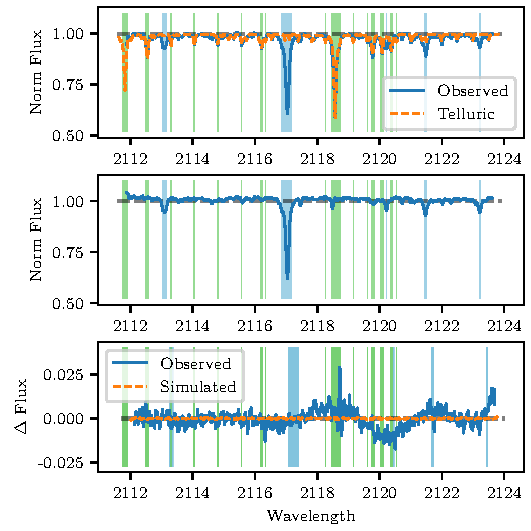
\includegraphics[width=0.8\hsize]{figures/direct-recovery/differential.pdf}\\
    \caption{(Top) A reduced {CRIRES} observation of {HD 30501} (blue) for detector 1 between 2\,112--2\,124\nm{} along with the tapas telluric absorption model ({orange} dashed) used for the wavelength calibration and telluric correction. (Middle) The telluric corrected spectra. (Bottom) ({blue}) Differential spectra for {HD 30501} between observations 1 and 3. ({orange} dashed) Simulated ``perfect'' differential using {PHOENIX-ACES} spectra with parameters \(\teff{} = 2\,500\K{}\), \(\logg{}=5.0\), and \(\feh{}=0.0\), with the same \(\Delta {RV}\) as the observations. The shaded regions indicate where the telluric {green} and host star {blue} spectra are > 4\% deep.}
    \label{fig:spectral_example}
\end{figure}


\subsection{Relative differential amplitude}
To probe this issue further we investigated how the amplitude of the differential signal changed with \(\Delta {RV}\). Taking the same {PHOENIX-ACES} spectra (\(\teff{} = 2\,500\K{}\), \(\logg{}=5.0\), \(\rm \feh{}=0.0\)), we computed differential spectra for a range of \(\Delta {RV}\)s between \(\pm10\)\kmps{}. \fref{fig:diff_amp} shows how the relative amplitude of the differential spectrum in the wavelength range 2\,110--2\,123\nm{} (detector 1 of our {CRIRES} observations) changed as the spectra are offset. At each {RV} step we take the maximum absolute differential value found. These are then normalized by the median value outside of the line {FWHM} (dashed vertical lines), between \(\pm(7-10)\)\kmps{}, to give a relative differential amplitude, independent from the depth of a specific line. For comparison we also show the relative amplitude of the differential spectrum for a single Gaussian and single Lorentzian line when Doppler shifted by the same \(\Delta {RV}\)s. The shape of these results is also consistent with the analytical form of the differential spectra~\citet[][eqn.~A.1]{ferluga_separating_1997}.

At a \(\Delta {RV}\) difference of zero, spectral lines of the companion completely cancel each other out, resulting in zero amplitude. As the {RV} separation increases, the individual lines stop cancelling themselves until a maximum differential amplitude is achieved when the lines are fully separated from themselves (equal to the line depth).

The two solid vertical lines in \fref{fig:diff_amp} indicate the estimated \(\Delta \textrm{RV}\)=1.34\kmps{} separation for our best target, {HD 30501} from \tref{tab:flux_table}, given known orbital parameters and the observation times. This shows that our differentials have severely reduced amplitude, \(<20\%\) relative to well separated individual lines. As the companion spectra are faint and in combination with a host star at 1\% flux ratio the >80\% extra reduction in signal amplitude makes this detection impossible with these observations.

In the synthetic spectrum (and of course real spectra) neighbouring spectral lines begin to interfere, leading to an impact on the measured relative amplitude. We suspect that the interaction of neighbouring lines is one possible cause for the difference between the theoretical and simulated shape between 2 and 6\kmps{}. Beyond the {RV} range present the amplitude becomes complicated due to neighbouring line interaction, but as the \(\Delta {RV}\) for all our spectra fall well short of this region we did not investigate this further.

\begin{figure}
    \centering
    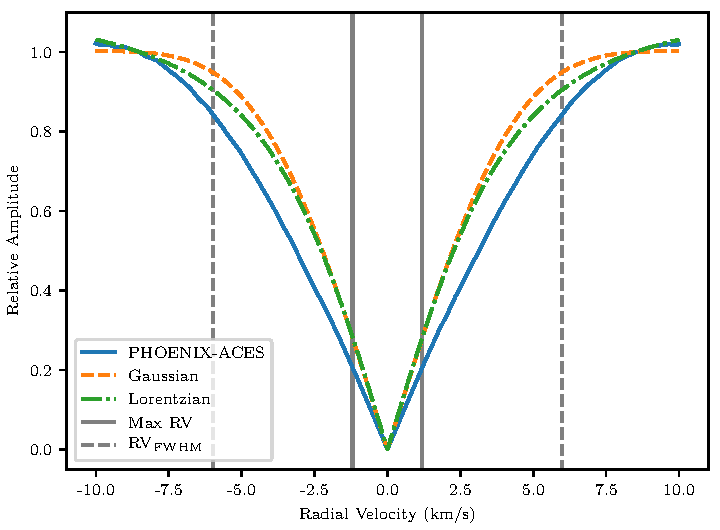
\includegraphics[width=0.45\textwidth]{figures/direct-recovery/rv_diff_final.pdf}
    \caption{Simulated relative amplitude of differential spectra at different {RV} separations revealing the diminished amplitude at small orbital separations. The solid blue line shows the maximum relative amplitude of the differential signal (from a shifted copy of itself) of a {PHOENIX-ACES} spectrum with \(\teff{}=2500\K{}, \logg{}=5.0, \feh{}=0.0\) in the wavelength region 2\,110--2\,123\nm{}. The maximum difference is normalized by the average amplitude between 7--10\kmps{}, representing a complete line separation. The orange (dashed) and green (dot-dashed) lines represent the relative amplitude of a differential spectrum of a spectrum containing a single Gaussian and single Lorentzian absorption line respectively, each with a unitary amplitude and a \(\rm {FWHM} = \lambda / R\). Beyond the {FWHM} lines the difference of the synthetic spectrum becomes more complicated due to the interaction of neighbouring lines. The solid vertical lines indicate the estimated companion \(\Delta {RV}\) in these observations while the dashed vertical lines indicate the {RV} corresponding to the {FWHM} at this wavelength and resolution. Beyond the {FWHM} {RV} the synthetic spectrum becomes complicated due to the interaction of neighbouring lines.}
    \label{fig:diff_amp}
\end{figure}
\unfinished{Increase size of diff amp plots to two}

\unfinished{Try show differences for all targets /all chips?}



\section{Estimating Companion-host Flux ratio}

\unfinished{Move location / adjust from paper}
\label{compaion flux ration}
The companion-host flux or contrast ratio of the systems are calculated using \(\frac{F_{2}}{F_{1}} \approx 2.512^{m_{1}-m_{2}}\), where \(m_{1}\) and \(m_{2}\) are the magnitude of the host and companion respectively.\ \(m_{1}\) is the magnitude of the host in the literature, while \(m_{2}\) is obtained from stellar evolution models of~\citet{baraffe_evolutionary_2003, baraffe_new_2015}, using the companion mass (or \(M_{2}\sin{i}\)) and the host's age. If only the companion minimum mass is known then this will correspond to the flux ratio lower limit, (or worst case scenario). The models, interpolated to the companion mass, also provide a first estimate of companion properties such as \teff{}, \logg{}, \(R/R_{\odot}\) and the magnitude in many wavelength bands.
We use the \emph{K}-band magnitude specifically for this work to estimate the flux ratio between the host and companion using the host \emph{K}-band magnitude obtained from {SIMBAD}~\citep{wenger_simbad_2000}. Our flux ratio estimates are presented in table~\ref{tab:flux_table}.
The companion \teff{} and \logg{} values specifically are used to influence the selection of synthetic model grids to perform the \textchisquared{} analysis over.

\subsection{Baraffe tables}
A simple tool\footnote{Available at \url{https://github.com/jason-neal/baraffe_tables}} was created to estimate the host-companion flux ratio using the~\citep{baraffe_evolutionary_2003,baraffe_new_2015} evolution tables. The minimum requirements are the host star name, the companion mass and a stellar/system age. The host's name is used to query the {SIMBAD} database to obtain available stellar properties, specifically for this work the photometric \textit{K}-band magnitudes and parallax. There are several Baraffe tables for different stellar ages. If the age given does not correspond to a published table then interpolation between two tables is preformed. The table selected is interpolated to the companion mass provided and the entries returned.

There is also a script available which operates in reverse. Given a host name, age, and a flux ratio it will find the table position and corresponding companion mass that It can also work in reverse to estimate the companion mass when provided with a flux ratio value.




\section{Direct recovery in the {MIR}}
Early on in 2015 we began investigating extending this technique to the {MIR}. In particular looked at applying for observing time with a {MIR} instrument to perform a similar differential subtraction technique.
There were two reasons for this, to explore the {MIR} where the contrast ratios are higher and because we were unaware of high-resolution \nir{} instrument available, as {CRIRES} was being upgraded to {CRIRES+}.

We explored the use of {VISIR} to detect brown dwarf companions in the {MIR}. The candidate selected as the best to investigate was HD ....


Of the targets in the correct location XXX was deemed to be the best case.

Looking at the best candidates XXXX was chosen a a likely target. I calculated flux ratios and performance considerations we determined that observations with VISIR to achieve a {SNR} of 100 were unfeasible, requiring 1\,000's of hours observing time.

The goal would be to observe with High-resolution and high through-put spectrographs. Ideally with {CRIRES+}, which at the time was scheduled for 2017. Currently\footnote{June 2018} first light is scheduled for Q1 2019.




\subsubsection{Differential scheduling challenges {copy from paper}}
\label{subsubsec:differential-schedualing}
This work has revealed that more care needs to be taken in planning the observations for the spectral differential analysis of faint companions in the future.
Paying attention in particular to the {FWHM} of the lines in the region (governed by resolution and wavelength); the estimated companion \(\Delta {RV}\); the previous observations from different observing periods; and keeping consistent detector settings.

The original goal for the observations was to obtain two different and ``clearly separated radial-velocities'' for the secondary companion.
However, the program was assigned a low-priority (C, in ESO grading) and, possibly due to operational reasons, the original time requirements necessary to secure well separated RVs for the companion spectra could not be met.
This meant that all observations were insufficiently separated to extract a differential spectra for the companion.

The long orbital periods of these targets is also a contributing factor to the insufficient separations.
Most of the targets observed here have orbital periods much longer than an observing semester (183 days).
An optimal pair of observations (achieved at the extrema) would need to have been obtained from separate observing periods (between 2 months and 19 years apart).
In some cases, even observations taken at the beginning and end of the semester would not be sufficient to achieve companion separation (depending on the phase).
Requiring separate observing periods to even achieve the minimum \(\Delta \rm {RV}\) larger than the line {FWHM}.
At the time it was impossible to ask for time over several semesters in a regular proposal.

Our study demonstrates the importance of proposals for projects that need to be extended over several semesters or years. In the ESO context, this corresponds to ``Monitoring proposals''~\citep[e.g.,][pg. 18]{eso_eso_2017}.
Observations of the targets explored here, with long orbital periods in particular, would benefit from the ability for multi-period proposals and newer scheduling systems which allow for tighter scheduling constraints, such as a companion {RV} separation.

For future observations we suggest that the known orbital solution of the companion be used to estimate the companions' {RV} curve during the observing period, with the companion \(M_2\sin{i}\) providing an {RV} upper-limit.
Knowing the instrumental wavelength and resolution, a constraint can then be set to avoid taking observations when the companion spectra are insufficiently separated, or \(\Delta {RV}\) < {FWHM}.\@This constraint can be set using the absolute and relative \emph{time-link} constraints available in {ESO}'s {Phase 2 Proposal Preparation} (P2PP) tool.
Additionally, analysing the known orbital solution before-hand, to determine {RV} constraints will also help identify the best time to observe, if observations from separate periods will be required or, if an optimally separated companion differential is even feasible.


It was unable to be determined if the time differential was asked for in the 2nd proposal....


\section{Orbital variations}

The insufficient spacing becomes clear when the RV variation during the orbits are visualized. Figures~\ref{fig:hd4747p89}--\ref{fig:hd30501p89} show the RV curves for each target.
Stars with two companions are shown twice, with each companion treated as a single Keplerian (ignoring the presence of the other companion).
For each panel on the left hand plot shows the RV variation across a orbit of the companion, while the panel on the right shows the RV variation for the 6 months observation window of Period 89.
The solid black line indicates the RV of the host star (with scale on the left), while the blue dashed line shows the RV of the companion (with scale on the right axis).
The orange crosses and red stars indicate the times at which observations were obtained for each target, for the host and companion respectively.

they show the phase placements, etc.

the companions are calculated by ... eq ...

Orbital parameters are the values provided in \tref{tab:orbitparams}.

Some code to create plots like this is available on \textit{Github} under the iastro-pt/Observationtools \footnote{\href{https://github.com/iastro-pt/ObservationTools}{https://github.com/iastro-pt/ObservationTools}} repository with documentation on \href{Read the Docs}{https://ia-observationtools.readthedocs.io/en/latest/rv.html}.



The sampling of points in the RV curve reveal that the choice of points was not favourable...

\todo{change RV scale for hd4747 orbit}

\begin{figure}
    \centering
    \begin{tabular}{cc}
    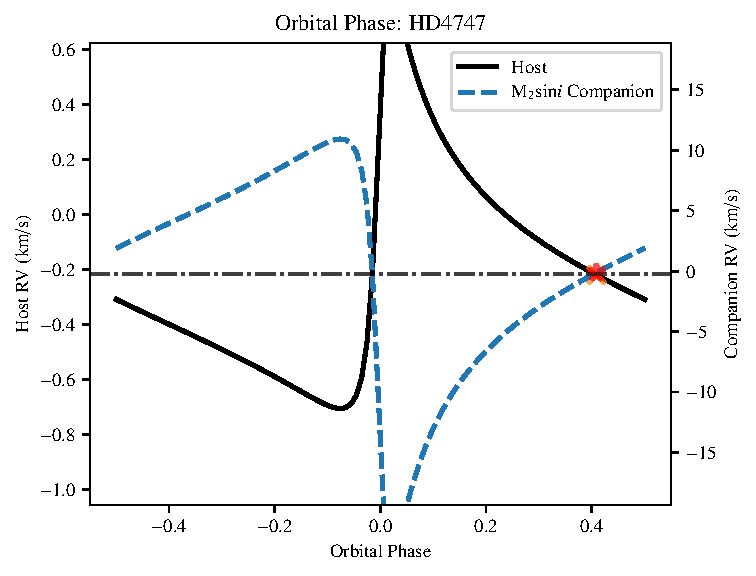
\includegraphics[width=0.45\linewidth]{figures/direct-recovery/orbital-plots/HD4747_orbital_phase.pdf}& 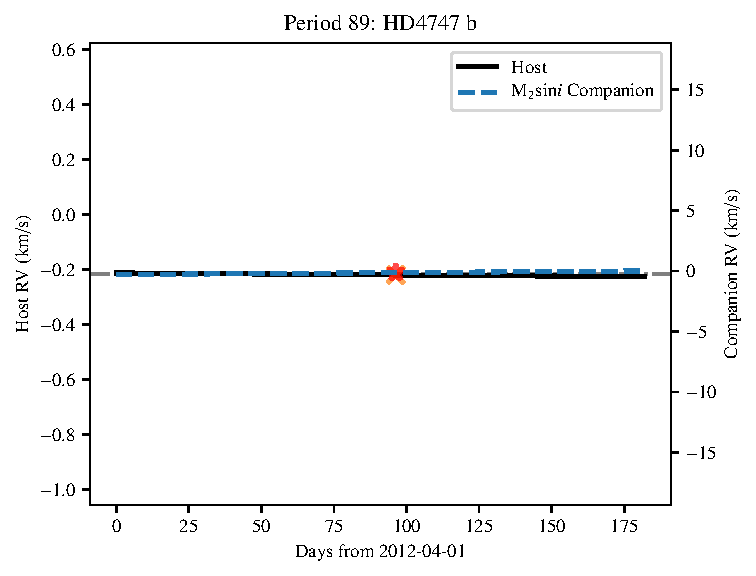
\includegraphics[width=0.45\linewidth]{figures/direct-recovery/orbital-plots/HD4747_p89.pdf}\\
    \end{tabular}
    \caption{RV orbital single companion Keplerian for the HD4747. The left hand shows the RV for a whole orbit of the target while the right hand panel shows the RV curve over 6 months (period 89). The solid black line indicates the RV of the host star (with scale on the left), while the blue dashed line indicates the RV of the companion (with scale on the right axis).  The orange crosses and red stars indicate the times at which observations were obtained for the target, for the host and compnaion respectively.}
    \label{fig:hd4747p89}
\end{figure}

\begin{figure}
    \centering
    \begin{tabular}{cc}
        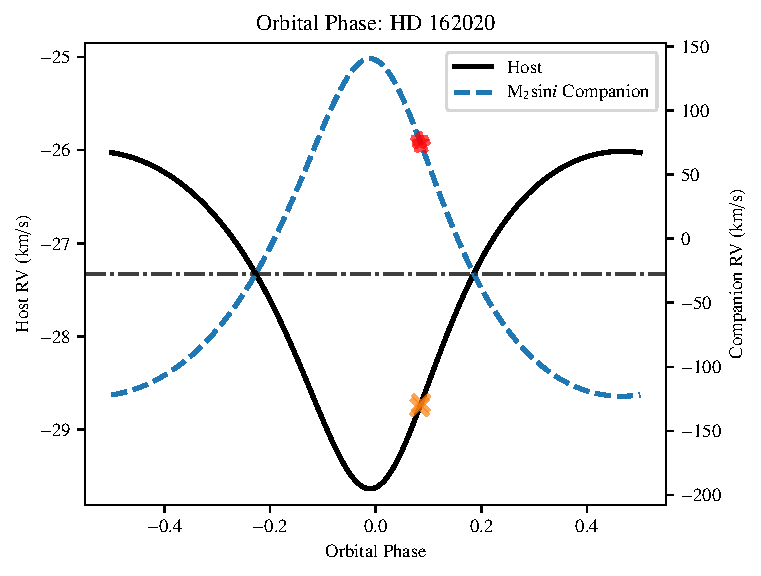
\includegraphics[width=0.45\linewidth]{figures/direct-recovery/orbital-plots/HD162020_orbital_phase.pdf}&
        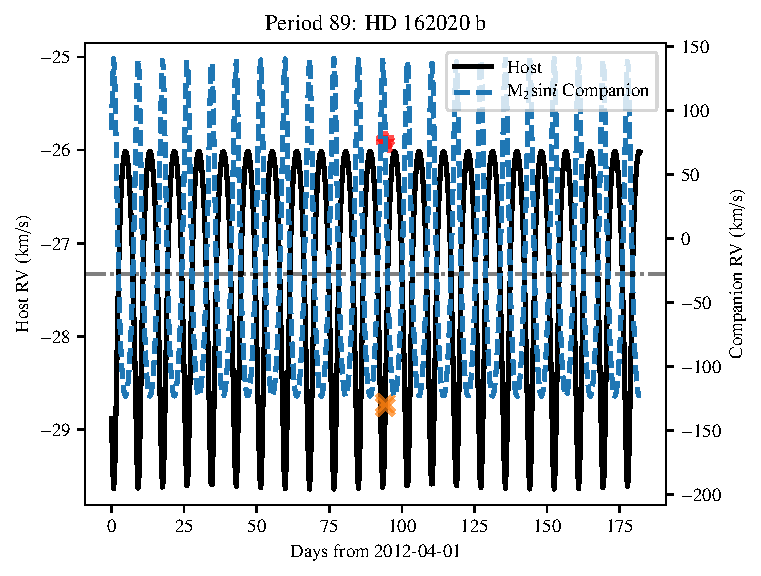
\includegraphics[width=0.45\linewidth]{figures/direct-recovery/orbital-plots/HD162020_p89.pdf}\\
    \end{tabular}
    \caption{Same as \fref{fig:hd4747p89} but for HD 162020.}
    \label{fig:hd162020p89}
\end{figure}

\begin{figure}
    \centering
    \begin{tabular}{cc}
        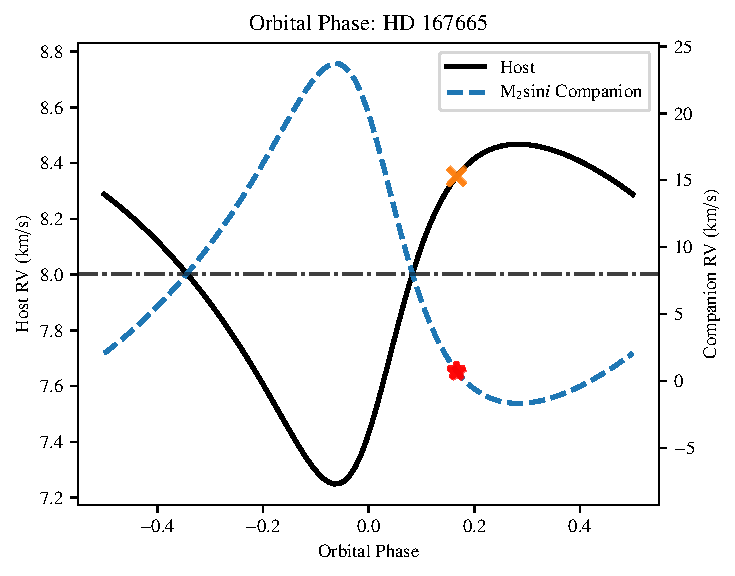
\includegraphics[width=0.45\linewidth]{figures/direct-recovery/orbital-plots/HD167665_orbital_phase.pdf}&
        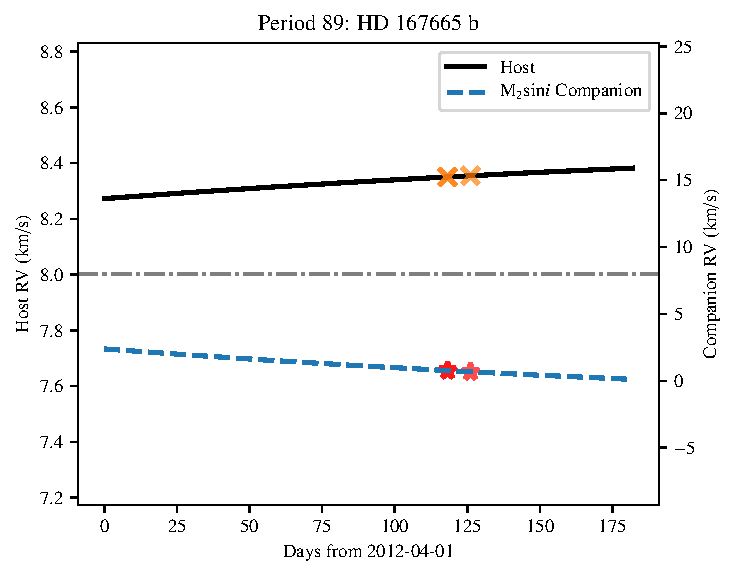
\includegraphics[width=0.45\linewidth]{figures/direct-recovery/orbital-plots/HD167665_p89.pdf}\\
    \end{tabular}
    \caption{Same as \fref{fig:hd4747p89} but for HD 167665.}
    \label{fig:hd167665p89}
\end{figure}

\begin{figure}
    \centering
    \begin{tabular}{cc}
        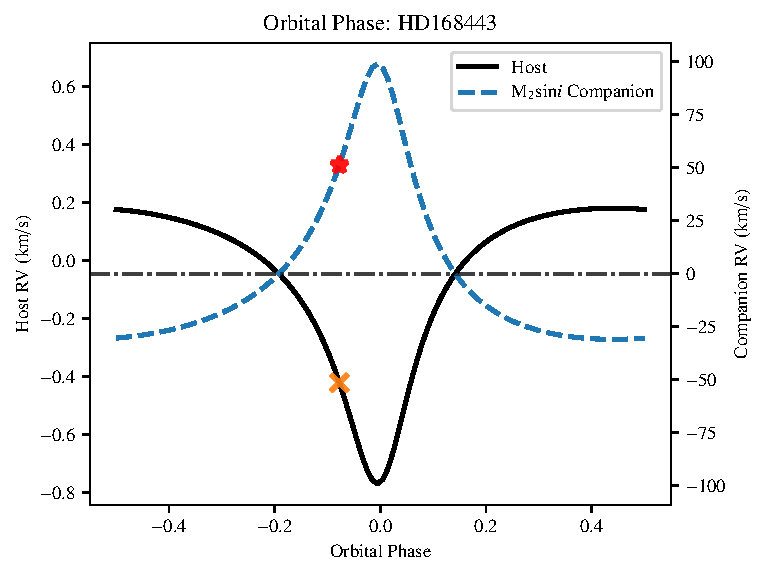
\includegraphics[width=0.45\linewidth]{figures/direct-recovery/orbital-plots/HD168443b_orbital_phase.pdf}&
        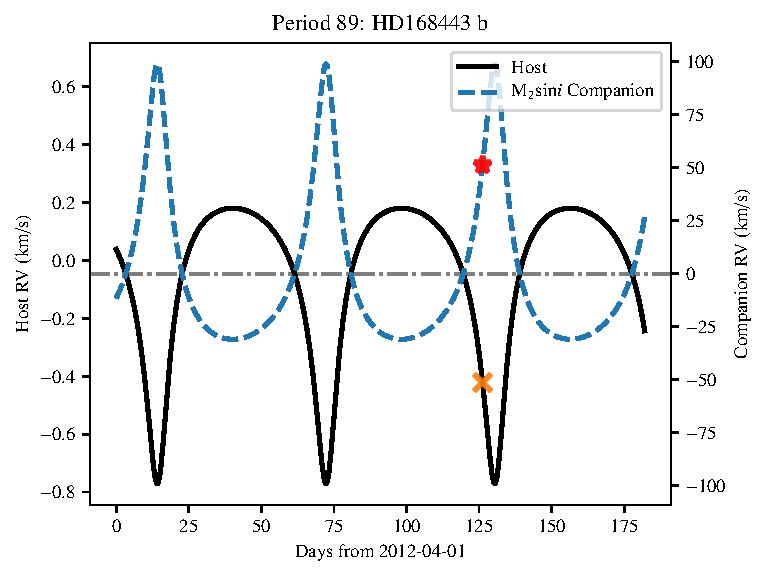
\includegraphics[width=0.45\linewidth]{figures/direct-recovery/orbital-plots/HD168443b_p89.pdf}\\
    \end{tabular}
    \caption{Same as \fref{fig:hd4747p89} but for HD 168443b.  Analysed as if this was a single companion.}
    \label{fig:hd168443bp89}
\end{figure}


\begin{figure}
    \centering
    \begin{tabular}{cc}
        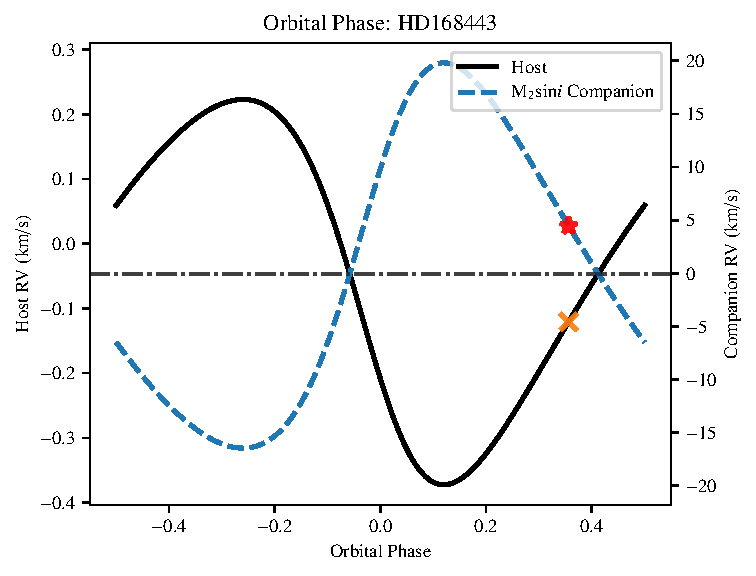
\includegraphics[width=0.45\linewidth]{figures/direct-recovery/orbital-plots/HD168443c_orbital_phase.pdf}&
        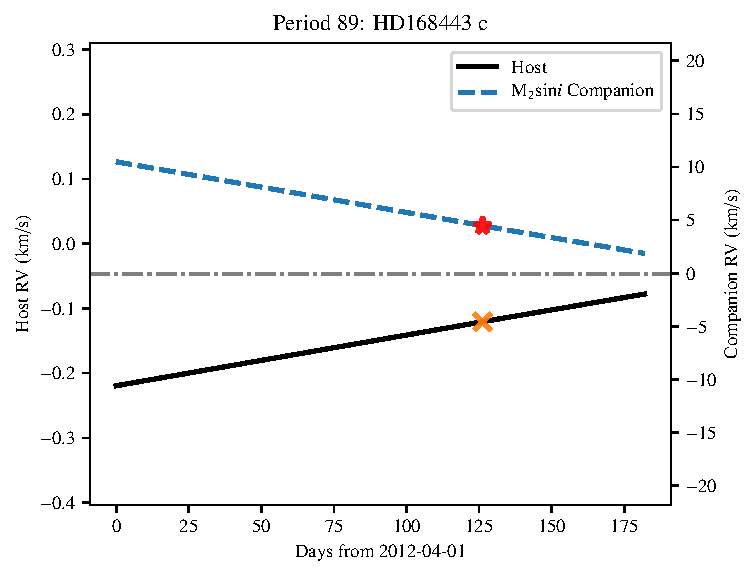
\includegraphics[width=0.45\linewidth]{figures/direct-recovery/orbital-plots/HD168443c_p89.pdf}\\
    \end{tabular}
    \caption{Same as \fref{fig:hd4747p89} but for HD 168443c.  Analysed as if this was a single companion.}
    \label{fig:hd168443cp89}
\end{figure}

\begin{figure}
    \centering
    \begin{tabular}{cc}
        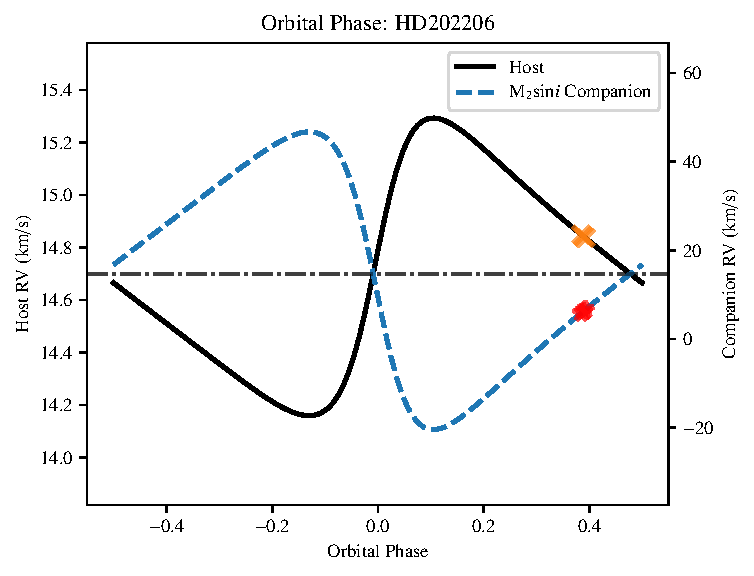
\includegraphics[width=0.45\linewidth]{figures/direct-recovery/orbital-plots/HD202206B_orbital_phase.pdf}&
        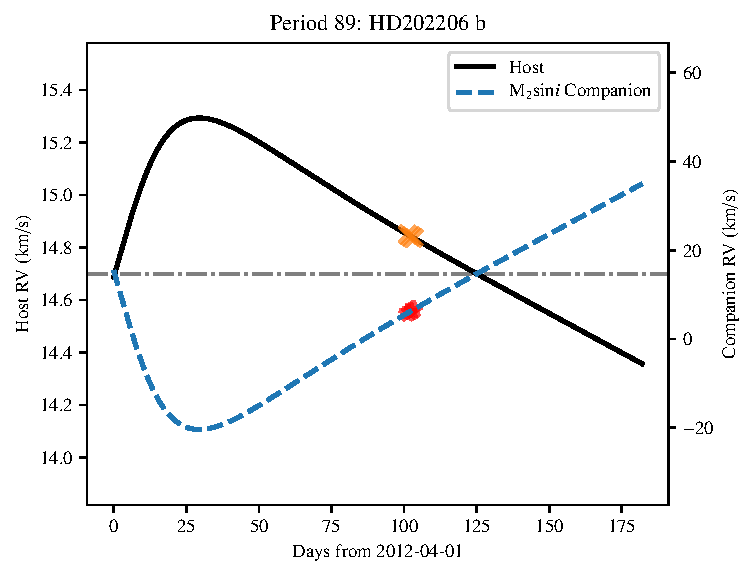
\includegraphics[width=0.45\linewidth]{figures/direct-recovery/orbital-plots/HD202206B_p89.pdf}\\
    \end{tabular}
    \caption{Same as \fref{fig:hd4747p89} but for HD 202206B. Analysed as if this was a single companion.}
    \label{fig:hd202206bp89}
\end{figure}

\begin{figure}
    \centering
    \begin{tabular}{cc}
        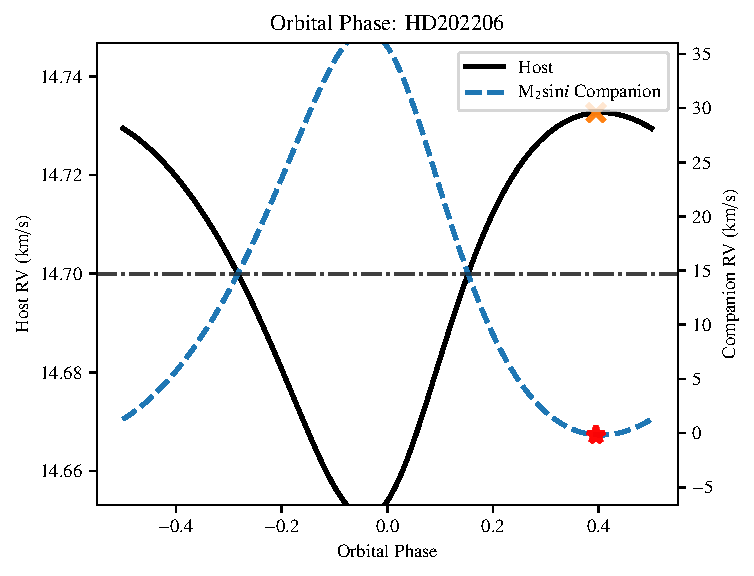
\includegraphics[width=0.45\linewidth]{figures/direct-recovery/orbital-plots/HD202206c_orbital_phase.pdf}&
        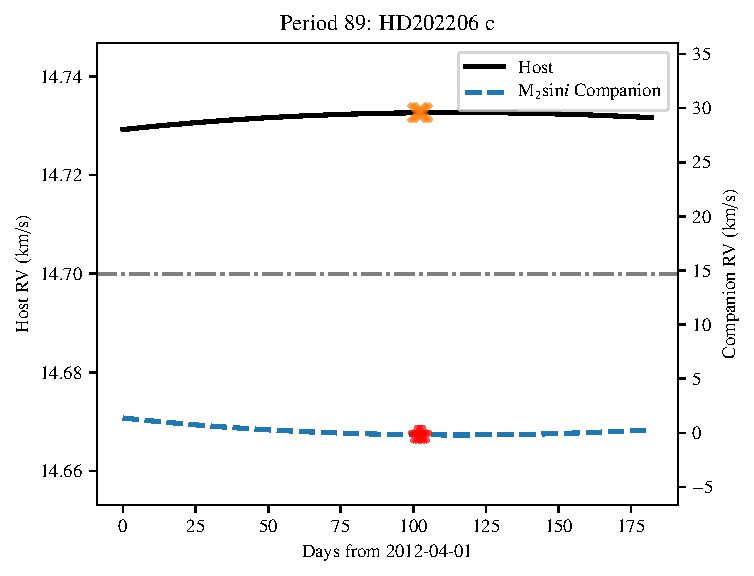
\includegraphics[width=0.45\linewidth]{figures/direct-recovery/orbital-plots/HD202206c_p89.pdf}\\
    \end{tabular}
    \caption{Same as \fref{fig:hd4747p89} but for HD 202206c. Analysed as if this was a single companion. }
    \label{fig:hd202206cp89}
\end{figure}

\begin{figure}
    \centering
    \begin{tabular}{cc}
        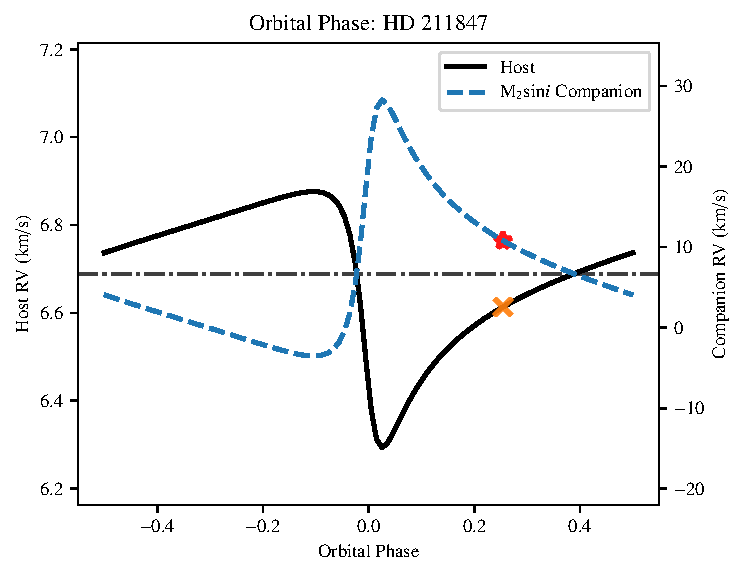
\includegraphics[width=0.45\linewidth]{figures/direct-recovery/orbital-plots/HD211847_orbital_phase.pdf}&
        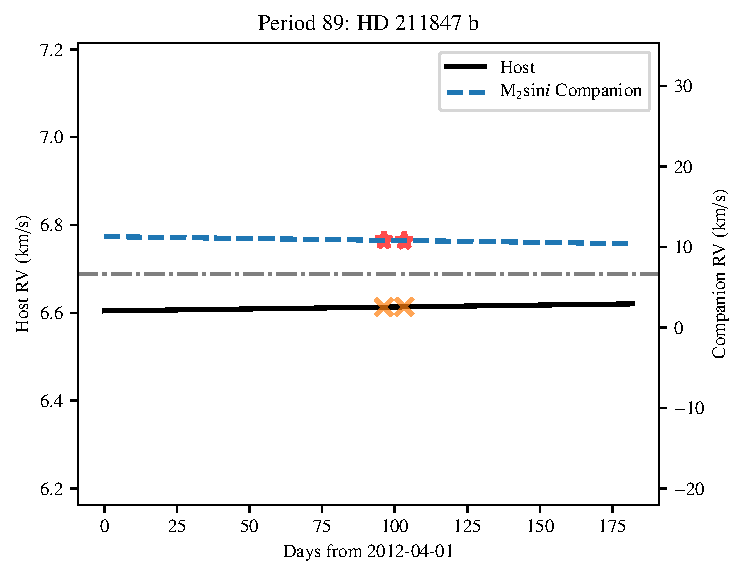
\includegraphics[width=0.45\linewidth]{figures/direct-recovery/orbital-plots/HD211847_p89.pdf}\\
    \end{tabular}
    \caption{Same as \fref{fig:hd4747p89} but for HD 211847.}
    \label{fig:hd211847p89}
\end{figure}

\begin{figure}
    \centering
    \begin{tabular}{cc}
        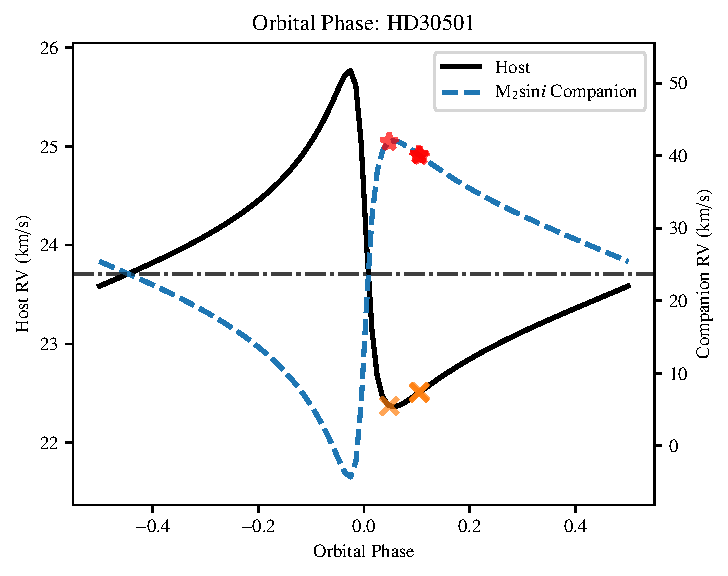
\includegraphics[width=0.45\linewidth]{figures/direct-recovery/orbital-plots/HD30501_orbital_phase.pdf}&
        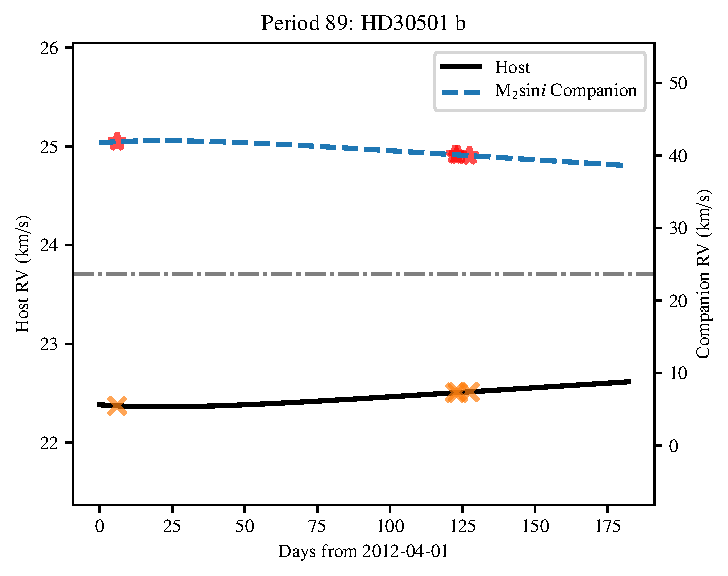
\includegraphics[width=0.45\linewidth]{figures/direct-recovery/orbital-plots/HD30501_p89.pdf}\\
    \end{tabular}
    \caption{Same as \fref{fig:hd4747p89} but for HD 30501.}
    \label{fig:hd30501p89}
\end{figure}
\todo{Check M2sini labels - can we get M2 only for those that we know}


\todo{An example of varying inclination or changing mass. Can use to show how 2 points add further constraint to the RV curve}


\subsection{Estimating Companion-host Flux ratio}
\label{compaion flux ration}
The companion-host flux or contrast ratio of the systems are calculated using \( \frac{F_{2}}{F_{1}} \approx 2.512^{m_{1}-m_{2}} \), where \(m_{1} \) and \(m_{2} \) are the magnitude of the host and companion respectively. The noise ratio between the host and companion is also calculated using \(N_{2}/N_{1} = \sqrt{2} \times\sqrt{F_{1}/F_{2}}\).  For this work we specifically use the magnitudes in \textit{K}-band. The magnitudes of the hosts, \(m_{1} \), are obtained from SIMBAD~\citep{wenger_simbad_2000} while the magnitudes for the companions, \(m_{2} \), are estimated from stellar evolution models~\citet{baraffe_evolutionary_2003, baraffe_new_2015}. The stellar evolution models are interpolated to the companion mass (or \(M_{2}\sin{i}\)) and system age, then the magnitude in the \textit{K}-band magnitudes extracted. The \textit{K}-band magnitudes, used for the host and companions along with the calculated flux ratio for each target is given in Table~\ref{tab:estimatedparameters}. For the companions in which only the minimum mass is known then the flux-ratio will be the lower limit, or worst case scenario.

These evolution models also provide a first estimate of the companions other properties such as \teff{}, \logg{}, \(R/R_{\odot}\) and the magnitude in many other wavelength bands.  The companion \teff{} and \logg{} values specifically were utilized to influence the selection of synthetic model grids to perform the \(\chi^2\) analysis over in Section~\ref{sec:results}.

A simple tool\footnote{Available at \url{https://github.com/jason-neal/baraffe_tables}} was created to calculate the flux ratio using the~\citep{baraffe_evolutionary_2003,baraffe_new_2015} evolution tables. Given the host star name, the companion mass and a stellar age it interpolates the available Baraffe tables to the companion mass and age specified. The host's name is used to query the {SIMBAD} database to obtain stellar properties, specifically magnitudes, to calculate the flux ratios. It can also work in reverse to estimate a companion mass when provided with a flux ratio.



%!TEX root = ../thesis.tex
\begin{table*}
	\centering
	\small
	\caption{Stellar parameters of the target companion's host stars.}
		\begin{tabular}{l c c r@{$~\pm~$}l r@{$~\pm~$}l r@{$~\pm~$}l r@{$~\pm~$}l r@{$~\pm~$}l c}
		\toprule
		Star & SpT & V &  \multicolumn{2}{c}{\(T_{\textrm{eff}}\) (K)} &  \multicolumn{2}{c}{logg (cm s\(^{-2} \))} & \multicolumn{2}{c}{[Fe/H]} &  \multicolumn{2}{c}{\(M_1\) (M\(_{\sun} \))} & \multicolumn{2}{c}{Age (Gyr)} & Reference\\
		\midrule
        \object{HD 4747}     & K0V & 7.15 & 5316 & 50 & 4.48 & 0.10  & $-$0.21 & 0.05 & 0.81 & 0.02  & 3.3   & 2.3 & 1, 2, 3\\ 
		\object{HD 162020} & K3V & 9.12 & 4723 & 71 & 4.31 & 0.18  & $-$0.10 & 0.03 & 0.74 & 0.07  & 3.1   & 2.7 & 4, 5    \\  
		\object{HD 167665} & F9V & 6.48 & 6224 & 50 & 4.44 & 0.10  & 0.05       & 0.06 & 1.14 & 0.03  & 0.7   & 3.6 & 1        \\
		\object{HD 168443} & G6V & 6.92 & 5617 & 35 & 4.22 & 0.05 & 0.06       & 0.05 & 1.01 & 0.07  & 10.0 & 0.3 & 5, 6    \\ 
		\object{HD 202206} & G6V & 8.07 & 5757 & 25 & 4.47 & 0.03 & 0.29       & 0.02 & 1.04 & 0.07  & 2.9   & 1.0 & 5, 7    \\ 
		\object{HD 211847} & G5V & 8.62 & 5715 & 24 & 4.49 & 0.05  & $-$0.08 & 0.02 & 0.92 & 0.07  & 0.1   & 6.0 & 2, 4    \\ 
		\object{HD 30501}   & K2V & 7.59  & 5223 & 50 & 4.56 & 0.10 & 0.06       & 0.06 & 0.81 & 0.02  & 0.8   & 7.0 & 1, 4    \\ 
		\bottomrule
	\end{tabular} \\
	\tablebib{
	          (1) \citet{sahlmann_search_2011}; (2) \citet{santos_spectroscopic_2005}; (3) \citet{crepp_trends_2016}; (4) \citet{tsantaki_deriving_2013}; (5) \cite{bonfanti_age_2016}; (6) \citet{santos_spectroscopic_2004};
	          (7) \citet{sousa_spectroscopic_2008};
	          }
	\label{tab:starparams}
\end{table*}
%!TEX root = ../thesis.tex
% Table of orbit parameters

\todo{Rotate orbital parameter table.}
\begin{table*}
		\centering
		\tiny
		\caption{Orbital parameters for the BD companions obtained from the literature.}
		\begin{tabular}{l c r@{$ \,\pm\, $}l r@{$ \,\pm\, $}l r@{$ \,\pm\, $}l r@{$ \,\pm\, $}l r@{$ \,\pm\, $}l cc c c}
		\toprule
		Object  & \(\gamma \)  	& \multicolumn{2}{c}{Period}   & \multicolumn{2}{c}{\(e \) } &  \multicolumn{2}{c}{\(\textrm{K}_{1} \) } &  \multicolumn{2}{c}{\(T_{0} \)}  &  \multicolumn{2}{c}{ \(\omega \) } & \(M_2\sin{i}\) & \(M_2\) & Ref.\\
		 & (km\(^{-1} \)) 	& \multicolumn{2}{c}{(day)}   	&    \multicolumn{2}{c}{}    &  \multicolumn{2}{c}{(ms\(^{-1} \))}   & \multicolumn{2}{c}{ (JD-2,450,000) } &  \multicolumn{2}{c}{(deg) } &   \(\rm {M}_{Jup} \)  &   \(\rm {M}_{Jup} \)   & \\
		\midrule
		\object{HD 4747}       & $0.215 \pm 11 $        	 &  13826.2  &  314.1            &  0.740 & 0.002  	& 755.3   &  12      & 463.1       &  7.3    & 269.1      &  0.6   &  39.6    & 60.2 			  & 1 \\
		\object{HD 162020}   & $-27.328\pm0.002$  	    &  8.42819  &  $6e^{-5}$   &  0.277 & 0.002   & 1813    &  4        & 1990.68   &  0.01  & 28.4        &  0.2   & 14.4     &     -   			  & 2 \\
		\object{HD 167665}   & $8.003 \pm 0.008$    	 & 4451.8 & 27.6   				   & 0.340 & 0.005 	  & 609.5   &  3.3     & 6987.6     &  29     & $-$134.3 & 0.9     & 50.3    &     -    			& 3 \\
		\object{HD 168443}b  & $-0.047\pm0.552$ 		& 58.1124 & $4e^{-4}$  		& 0.529 & 0.001   & 475.13 & 0.9      & 5626.20  &  0.02   & 172.9      & 0.1     & 7.7      &     -    			& 4 \\ 
		\object{HD 168443}c  & $-0.047\pm0.552$ 		 & 1749.83 & 0.57  			     & 0.211 & 0.002  	 & 297.7  & 0.6      & 5521.3     &  2.2     & 64.9       & 0.5     & 17.1    &     -    			  & 4 \\ 
		\object{HD 202206}B & 14.721     						& 256.33  &  0.02    		     & 0.432 & 0.001  	  & 567     &  1       & 2176.14    &  0.12   & 161.9     & 0.2  	& 17.4    & $93.2\pm7.3$   & 5, 6\\  
		\object{HD 202206}c & 14.721    						 & 1260 &  11			        	& 0.22 & 0.03 		  & 41    	& 1          & 3103 		& 452    & 280 		   & 4  	  & 2.3      & $17.9\pm2.9$  & 5, 6\\ 
		\object{HD 211847} 	 & 6.689\tablefootmark{a} & 7929.4 & 2500  		    	 & 0.685 & 0.068   	  & 291.4   & 12.2   & 12030.1    & 2500   & 159.2 		& 2.0     & 19.2  & 155  				& 3, 7\\
		\object{HD 30501}  	  & $23.710\pm0.028$         & 2073.6 & 3.0 				& 0.741 & 0.004   	   & 1703.1 & 26.0   & 3851.5 		& 3.0     & 70.4 		& 0.7     & 62.3   & 89.6      			& 3  \\
		\bottomrule
	\end{tabular}
	\tablebib{
	          (1) \citet{crepp_trends_2016}; (2) \citet{udry_coralie_2002}; (3) \citet{sahlmann_search_2011}; 
	          (4) \citet{pilyavsky_search_2011}; (5) \citet{correia_coralie_2005};  (6) \citet{benedict_hd_2017}; (7) \citet{moutou_eccentricity_2017}
	}
	\tablefoot{
	\tablefoottext{a}{fixed}
	}
	\label{tab:orbitparams}
\end{table*}



CHECK out LOCKWOOD 2014 - maximum likelihood with todcor 1e-4 flux ratio double lined spectra

	%!TEX root = ../thesis.tex
%4-Snellen/Brogi analysis
% ability to detect singal??


\chapter{Companion Recovery using synthetic models}  % Main chapter title
\label{cha:model_comparison}

Because the differential subtraction technique was unsuccessful, not being separable in time, a second method was attempted to try and extract something useful out of the spectra.

We develop this new method, preform some tests and then show the results obtained.
There were numerous issues encountered and unsuccessful results.

Contrast our result to other works.  More phases, longer integration time, higher {SNR}.




\section{Binary synthetic spectral recovery}
\label{subsec:companion_recovery}
Since the differential method is ineffective for our dataset due to the {RV} separation between observations, we explored a second approach to detect the presence of the faint companion spectra.
This second approach compares the observed spectra to combinations of synthetic spectral models using \textchisquared{} methods which have been extensively used in the literature~\citep[e.g.][]{astudillo-defru_harps_2015, passegger_fundamental_2016, zechmeister_spectrum_2018, nemravova_xtauri_2016, kolbl_detection_2015}. {\red{} The temperature of synthetic spectra fitted to the companion will provide some indication of the companions spectral type, but will not produce a direct mass constraint that was the original aim of this work.}

\subsection{\texorpdfstring{\textchisquared}\ \ method}
\label{subsec:chi2}
The well known \textchisquared{} technique measures the weighted sum of the squared deviation between the observation (\({O}_{i}\)) and the computed models (\(C_{i}\)), with the minimum \textchisquared{} value representing the best-fit parameters:
\[\chisquared = {\sum}_i \frac{{(O_{i} - C_{i})}^2}{{\sigma}_{i}},\] where \({\sigma}_{i}\) is the error on each measurement.
We estimate the \(\sigma\) of each spectrum using the \(\beta\sigma\) method~\citep{czesla_posteriori_2018}, using the MAD (median absolute deviation about the median) robust estimator. {\red{} This method estimates the spectral noise using numerical derivatives of the spectra.
We followed the procedure outlined in~\citet{czesla_posteriori_2018}, analyzing the results from successive parameter combinations to settle on an order of approximation (derivative level) of 5, and a jump parameter (pixels skipped to avoid correlations) of 2.} We apply the same \(\sigma\) value to all points \({\sigma}_{i} = \sigma\).
The \(\beta\sigma\) method provided \(\sigma\) estimates for the target spectra which correspond inversely to signal-to-noise ratios between 100--500, {\red{} similar to the values given in \cref{tab:observations} calculated from the continuum of detector 2.}

The computed models are described in \cref{models} and result in a multidimensional grid of \textchisquared{} values for each combination of parameters, namely the spectral temperature, host {RV}, and companion {RV} for each detector, observation and target.

We obtain the global minimum of the multidimensional \textchisquared-space to represent the best fit to the observed spectra.
We sum the multidimensional \textchisquared{} across multiple detectors and determine a global minimum \textchisquared{} for the whole observation \(\chisquared_{obs} = \Sigma^{N}_{n=1} \chisquared_n\), where \(N\) is the number of detectors used.
We do not, however, combine the \textchisquared{} values across the separate observations as the {RV} parameters of the host and companion will vary between each observation.
However, since the current observations are insufficiently separated, it may be possible to combine the separate observations; but in general this would not be the case, so was not performed.

The inverse survival function of the \textchisquared{} distribution is used to determine the confidence levels on the minimum \textchisquared{} parameters.
The inverse survival function returns a \(\Delta\chisquared\) value from the minimum \textchisquared{} value for a given $\sigma$ level and degree of freedom\footnote{In \emph{Python} with the \emph{scipy} package this is a single line \texttt{scipy.stats.chi2{(dof)}.isf{(1-p)}}, where \(p = 0.68\) for 1-\(\sigma\), and dof is the degree of freedom.}.
For example, the \(\Delta \chisquared\) for a single degree of freedom required for the 1-, 2-, and 3-\(\sigma\) levels is 1, 4, and 9 respectively~\citep{bevington_data_2003}.
This method assumes that the measured flux is observed with a \snr{} sufficiently high so that the noise on the spectrum is approximately Gaussian, and the \textchisquared{} method appropriate.

For a given observation, the \(\chisquared_{red}\) is computed by \(\chisquared_{red} = \chisquared / \nu\) where \(\nu = n - m\), the number of observed pixels, \(n\), minus the number of parameters of interest, \(m\)\footnote{\(m=2\) or 4 in the examples explored below}, and is performed after the summation over the detectors.



%%%%%%%%%%%%%%%%%%%%%%%%%%%%%%%%%%%%%%%%%%%%%%%%%%%%%%%%%%%%%%%%%%%%%%%%%%%%%%%
%%%%%%%%%%%%%%%%%%%%%%%%%%%%%%%%%%%%%%%%%%%%%%%%%%%%%%%%%%%%%%%%%%%%%%%%%%%%%%%

\subsection{Computed model spectra}
\label{models}
In this section we detail how we transform the synthetic {PHOENIX-ACES} spectra into the computed models (\(C_i\)) to fit to the observations.
The spectra have already been converted to the correct unit and resolution.

These synthetic spectra are used individually for the single component model and combined together into a binary model.
The results of these models are interpolated to the wavelength grid of the observed spectra and the \textchisquared{} calculated by comparing the model and observation at each point.


{\red{} We multiply the synthetic spectra by the wavelength to convert it into photon counts, ignoring multiplicative constants, as done in~\citet{figueira_radial_2016}\footnote{Synthetic models provide the spectral energy distribution (\(\rm erg\,s^{-1}\,cm^{2}\,cm^{-1}\)).}.
The spectra were convolved with a Gaussian kernel to match the resolution of the observations (\(\rm R=50\,000\)).
Due to the distributive property of convolution it is efficient to apply it once to each spectra first, before the spectral pairs are combined.}


\subsubsection{Single component model}
\label{subsubsec:single-model}
The single model \(C^{1}_{i}\) comprises of a single synthetic spectrum, \(J\), (with model parameters \(\teff{}\), logg, \feh{}, [\(\alpha\)/\ce{Fe}]) and is Doppler shifted by a {RV} value \({rv}_1\).
\begin{equation}
\rm C^{1}_{i}(\lambda) = J(\lambda_0(1-\frac{{rv}_1}{c}))
\end{equation}
where \(\lambda\) is the shifted wavelength, \(\lambda_0\), the model rest wavelength and, \(c\), the speed of light in a vacuum.
The model's flux is then continuum normalized to unity to match the observed spectra, and interpolated to the wavelength grid of the observation.

This single component model analysis is similar to the~\citet{passegger_fundamental_2016} \textchisquared{} fitting.
We apply the same re-normalization (see \cref{subsec:renorm}) to account for slight differences in the continuum level and possible linear trends between the normalized observation and model.
We do not, however, apply any dynamical masking to sensitive lines to make the the \textchisquared{} minima more distinct or linearly interpolate the stellar parameters between the grid models to obtain high precision stellar parameters.
This is because we are not trying to derive precise stellar parameters but to detect the spectra of the companions.
We instead include radial velocity components to the \textchisquared{} fitting, which is not included in~\citet{passegger_fundamental_2016}.


\subsubsection{Binary model}
\label{subsubsec:binary-model}
In the binary situation we consider the superposition of two synthetic spectral components, one each for the host and companion respectively.
Both spectra are Doppler shifted by \({rv}_1\) which represents the {RV} motion of the host star, while the companion spectra is also Doppler shifted by a second {RV}, \({rv}_2\), representing the {RV} offset between the host and companion.
This choice is arbitrary, but in this way the mean motion of the system relative to Earth is captured only in \({rv}_1\).
The two spectra are scaled by their squared radius (see \cref{subsection-radius}) then added together, thus fixing the relative amplitude of the two components.
Given two spectral components \(J_{1}\)and \(J_{2}\)with radii \(R_1, R_2\) this equates to
\begin{align}
\rm C^{2}_{i}(\lambda) = &  J_{1}(\lambda_{0}(1 - \frac{rv_{1}}{c}))\times R_{1}^2 +\nonumber \\
& J_{2}(\lambda_{0}(1-\frac{rv_{1}}{c})(1-\frac{rv_{2}}{c}))\times R_{2}^2
\end{align}


The combined spectra is continuum normalized by dividing by an exponential fitted to the continuum of the combined spectrum, as we assume we are in the Rayleigh-Jeans regime.
This assumption here is wavelength dependent and other appropriate continuum normalization techniques are also valid.
In the case of a {BD} companion around an FGK star investigated here, the continuum is dominated by the contribution from the host star as it contributes the majority of the spectrum with flux ratios around 2\,110--2\,160\nm{} below \(\sim\)1\%.

We combine the models in this way to represent the correct absolute flux ratio of the components.
The median flux ratio between the two components is calculated for the wavelength range used here as an indication of the flux ratio level.

The binary model should provide meaningful information about the companion parameters (e.g.\ \(\teff{}\)) and an estimate of the flux ratio of the system.
These can be combined with the~\citet{baraffe_evolutionary_2003} models to constrain the mass of the companion.
However, we need to be careful with this model as the inclusion of extra spectral components and associated parameters could also provide a better fit to observations which do not have a companion, by fitting components of the noise.\\

{\red{} The full list of grid parameters for the binary model are \(\teffsub{1}\),  \(\logg{}_1\), \feh{}\(_1\), [\(\alpha\)/\ce{Fe}]\(_1\), \({rv}_1\), \(\teffsub{2}\), \(\logg{}_2\), \feh{}\(_2\), [\(\alpha\)/\ce{Fe}]\(_2\), \({rv}_2\) where the subscripts 1 and 2 indicate the host and companion models respectively.}






\subsubsection{Effective radius}
\label{subsection-radius}

To combine the two synthetic spectra with the correct observed flux ratio we need to integrate the emitted flux over the effective surface area of each emitting body respectively.
Ignoring the common multiplicative constants that will disappear with normalization, we scale the two synthetic spectra individually by the square of their respective radii, \(R_1\) and \(R_2\).

In this work we use the effective radius (PHXREFF keyword) of each component from the {PHOENIX} model headers.
This is the radius used in modelling the stellar atmospheres.
We use this radii as it is directly tied to each model spectrum, and already available.
The ratio of the radii from the two synthetic spectra in the binary models are provided in \cref{tab:example_params}.

We are aware that using these radii has its limitations since as stated previously: there is a degeneracy in {BD} mass, age, and luminosity of the companion, and in particular a combination of radius-mass and radius-age relationships~\citep{sorahana_radii_2013}.
Using the {PHOENIX-ACES} model effective radius does not allow for any independent age constraints to be incorporated, or allow for any variability in the radii to account for uncertainties.

The targets analysed here do not have transits, but if the radius ratio can be independently determined from the photometric transit method~\citep{deeg_photometric_1998} then this could be used to constrain the radius ratio used when combing the binary model spectra instead.


\subsection{Re-normalization}
\label{subsec:renorm}
Slight trends in the continuum level between the observed spectra and computed models were removed using the re-normalization following~\citet{passegger_fundamental_2016}:
\begin{equation}
F^{obs}_{re-norm} = F^{obs} \cdot \frac{\textrm{continuum fit}_{model}}{\textrm{continuum fit}_{observations}}.
\end{equation}
The polynomial continuum fits to the normalized observations and models are used to re-normalize the observed spectrum to the continuum of the models.
For detectors 1--3 a polynomial of first degree was used, while for detector 4 a quadratic is needed to fit the edge of a strong Hydrogen line (Brackett-\(\gamma\)) at 2\,166\nm{}, which lies just off of detector 4.
This broad line is only observed in the synthetic spectra and not in the reduced observations.
It is assumed that this was normalized out during the reduction process.

For each model we further allow the continuum level to be varied by \(\pm 0.05\) as a free parameter taking the model with the smallest \textchisquared{} value.


\subsection{Reducing parameters}
\label{subsec:reduce-params}
The high dimensionality of the binary model makes it computationally challenging and difficult to analyse the \textchisquared{} space.
For reference, the multiplicative parameter space is squared when increasing from one spectral component in the single model to a binary model, and therefore becomes computationally expensive.
In general the number of possible parameter combinations for \(c\) spectral components each with a grid of \(m\) models increases to \(c^m\).
If the full set of {PHOENIX-ACES} library spectra (66456) is explored with a binary fit then this naively balloons to over 4.4 billion possible combinations.
Half of these are not unique as the host and companion components are swapped.
This is the worst case scenario and we implement a number of assumptions to vastly reduce the parameter-space enabling faster computation.

Our first assumption is to restrict ourselves to models with an Alpha element abundance ([\(\alpha\)/\ce{Fe}]) of zero.
This is likely a very good approximation as all our targets have solar metallicity and are thus very likely to belong to the thin disk of the Galaxy, where [\(\alpha\)/\ce{Fe}] values are close to zero (i.e., solar)~\citet[e.g.]{adibekyan_chemical_2012}.
Our second is to assume that we can significantly reduce the search space with literature values for the host star.
We fix the metallicity of both components to the closest grid to the literature value (usually \feh{}=0.00).
We also fix the \logg{} of the host star to its literature values given in \cref{tab:starparams}.
The uncertainties on the literature measurements for \logg{} (\(\sim\)0.1) and metallicity (\(\sim\)0.05) are both smaller than the grid steps of 0.5 for these parameters.
The \logg{} of the companion is obtained from the~\citet{baraffe_evolutionary_2003,baraffe_new_2015} evolutionary models for the given companions \(\mtwo/\mtwosini\) and hosts age.

We use the estimated companion temperatures from the Baraffe evolutionary models given the companion (minimum) mass and stellar age as a starting point for the companion spectra grid computation and extend the grid in each direction, within the model limits.
For example we show the companion temperature grid spanning \(-600\) to \(+400\)\K{} in \cref{fig:Mdwarf_contours} and \(\pm400\)\K{} in \cref{fig:HD211847_simulated_contours, fig:HD211847_result_contours}.

The large numbers stated above also do not include the {RV} grid for each component.
The {RV} grid is user defined and the number of spectra /models to consider increases when the {RV} grid step size is decreased (finer {RV} resolution).
We can reduce the {RV} grid space significantly by tailoring it to the target being examined.
For each target, we use the estimated {RV} values from the observation time and orbital parameters, given in \cref{tab:observations} as a centre starting point for the \({rv}_1\) and \({rv}_2\) values and increment the {RV} within a few {\fwhm} around those values, or out to the targets \(\rm K_1\) and estimated \(\rm K_2\) values.

An iterative process could be implemented to refine the {RV} grids, starting at a larger grid with lower {RV} resolution then performing a higher resolution grid about the minimum \textchisquared{} {RV} values.
This was only done manually but could have been automated.
One could expect that a good starting {RV} grid step be governed by the spectral resolution, e.g.\ comparable to the {\fwhm} velocity.

For the companions targets with fully resolved orbits the known {RV} of the host star, \({rv}_1\) could also have been fixed.
We however left this free to see if the known value would be recovered by the fitting.





%%%%%%%%%%%%%%%%%%%%%%%%%%%%%%%%%%%%%%%%%%%%%%%%%%%%%%%%%%%%%%%%%%%%%
%%%%%%%%%%%%%%%%%%%%%%%%%%%%%%%%%%%%%%%%%%%%%%%%%%%%%%%%%%%%%%%%%%%%%

\todo{Example with a large mass companion? and/or SNR.}

\section{Results}
\label{sec:results}

%!TEX root = ../thesis.tex

\begin{table*}
      \centering
      \begin{threeparttable}
          \caption{Input and recovered parameters on simulations and an observation when applying a single (\(\rm C^1\)) and binary (\(\rm C^2\)) models. The \logg{} and metallicity were fixed at \(\logg{}_1 = 4.50\), \(\logg{}_2=5.0\) and \feh{}=0.0 equally for both components. Gaussian noise was added to both simulations with a \snr{} of 150. Here \(m\) and \(n\) are the number of data points and parameters used in each model.}

          \begin{tabular}{c | *3c | *3c | *3c}
              \toprule
              & \multicolumn{3}{c|}{Simulation 1} & \multicolumn{3}{c|}{Simulation 2} & \multicolumn{3}{c}{Observed {HD 211847}} \\
              \midrule
          & Input & \multicolumn{2}{c|}{Recovered} & Input & \multicolumn{2}{c|}{Recovered} & Expected & \multicolumn{2}{c}{Recovered} \\
          & & \(C^1\) & \(C^2\) & & \(C^1\) & \(C^2\) & & \(C^1\)  & \(C^2\) \\
          \midrule
          \(\teffsub{1}\) & 5\,800 & 5\,800 & 5\,800 & 5\,700 & 5\,800 & 5\,700 & \(5\,715 \pm 24\) & 5\,900 & 5\,800\\
          \(\teffsub{2}\) & 4\,000 & -- & 3\,800 & 3\,200 & -- & 3\,100 & \(\sim\)3\,200 & -- & >3\,800\tnote{a}\\
          \({rv}_1\) & 0 & 0.1 & 0 & 6.6 & 6.6 & 6.6 & \(6.6 \pm 0.3\) & 7& 7.6 \\
          \({rv}_2\) &  10 & -- & 9.8 & 0.5 & -- &  -1& \(0.5 \pm 2\) & -- &-12.6\\
          \midrule
          \(R_1/R_2\)& 2.57 & -- & 2.71& 3.16 & - & 3.27 & 3.16 & -- & <2.71\tnote{a}\\
          \(\rm F_2/F_1\)& 0.084 & -- & 0.066 & 0.030 & -- & 0.026 & 0.030 & -- & >0.066\tnote{a}\\
          \(m\) & - & 3\,072 & 3\,072 & -- & 3\,072 & 3\,072 & -- & 2\,612 & 2\,612\\
          \(n\) & - & 2 & 4 & -- & 2 & 4 & -- & 2 & 4\\
          \textchisquared& -- & 4\,978 & 3\,792 & -- & 3\,746 & 3\,630  & -- & 37\,688 & 33\,860\\
          \(\chisquared_{red}\) & -- & 1.62 & 1.24 & -- & 1.22 & 1.18 & -- & 21.3 & 19.2\\
          {BIC} & -- & -20\,145 & -22\,315 & -- & -21\,477 & -21\,377& -- & 18\,281 & 14\,468\\
          \bottomrule
        \end{tabular}\label{tab:example_params}
        \begin{tablenotes}
            \item [a] {At the arbitrary upper limit for companion temperature grid (3\,800\K{}).}
        \end{tablenotes}
    \end{threeparttable}
\end{table*}



\begin{figure*}
    \centering
    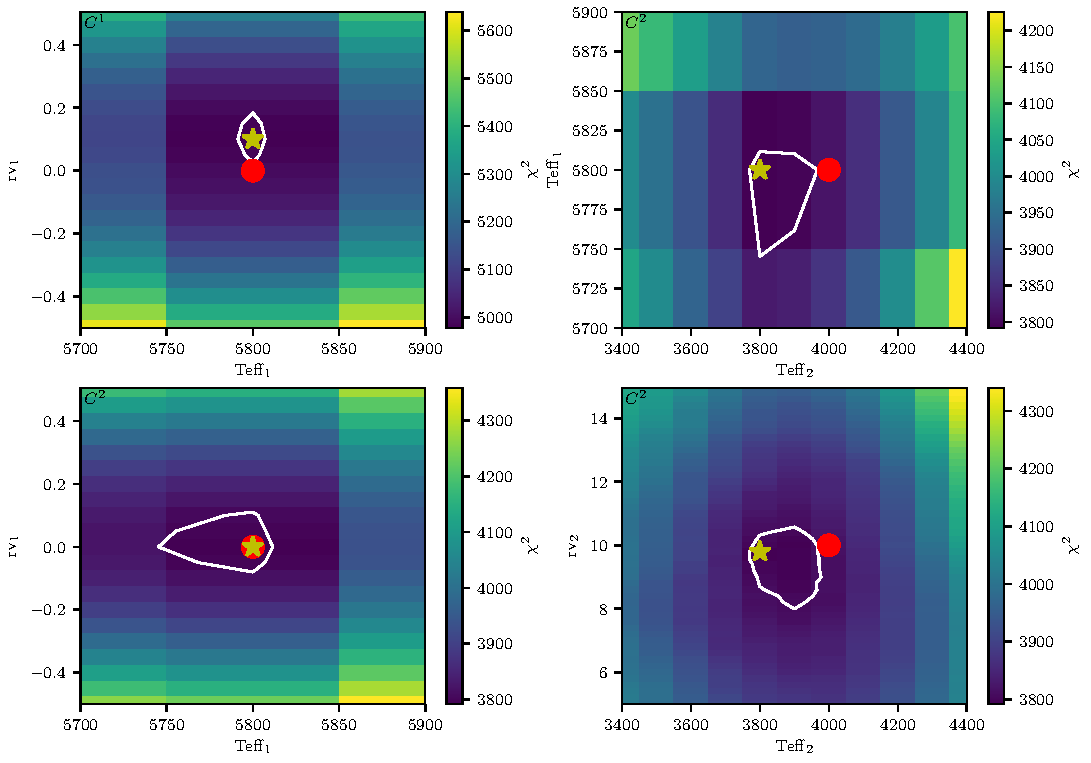
\includegraphics[width=0.7\linewidth]{figures/companion_recovery/Mdwarf_pcolors}
    \caption{\textchisquared{} results for companion recovery of a simulated binary observation of a Sun-like star (\(\teffsub{1}=5\,800\)\K{}) with an M-dwarf companion (\(\teffsub{2}=4\,000\)\K{}).
The top right plot shows the application of a single component model (\(C^1\)) while the other three are using a binary model (\(C^2\)).
Both left hand panels show the distribution of host temperature and host {RV}.\@ The top right panel shows the distribution for host and companion temperature, and the bottom right the companion temperature and radial velocity.
    The red circle and yellow star indicate the location of the simulation input and recovered parameters respectively.
    The white line shows a 3-\(\sigma\) confidence level about the minimum \textchisquared{} solution grid point.
Each box is centred on the parameter values and shows the grid resolution.}
    \label{fig:Mdwarf_contours}
\end{figure*}

\begin{figure*}
    \centering
    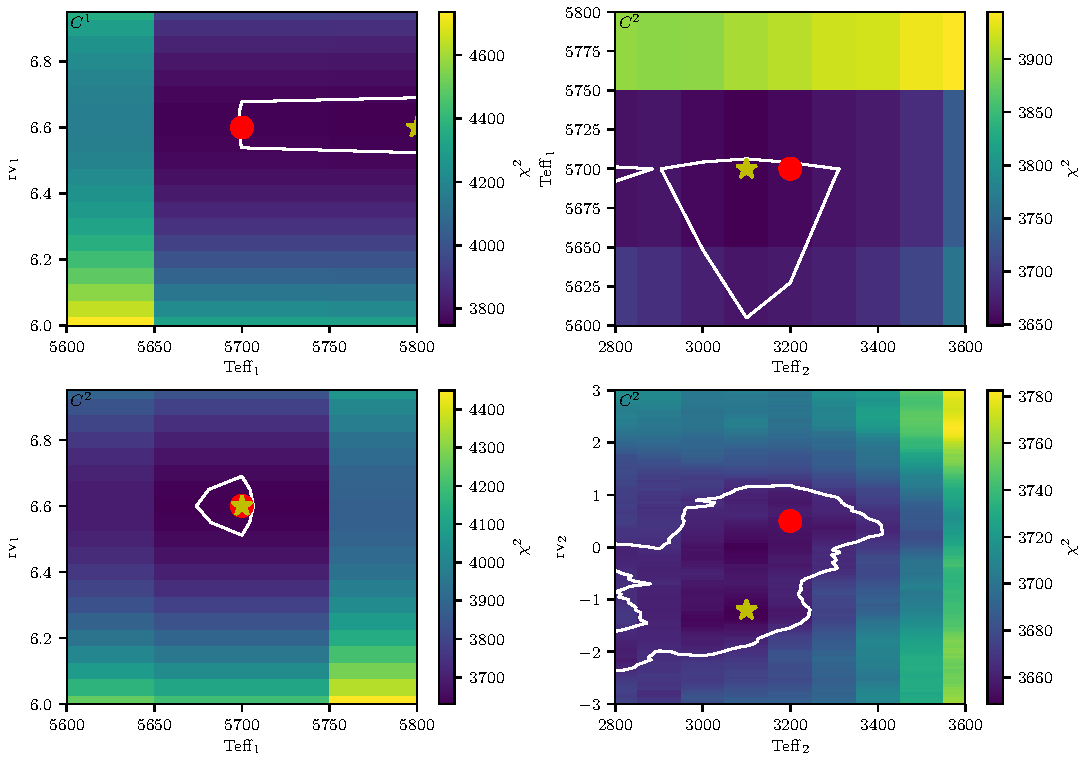
\includegraphics[width=0.7\linewidth]{figures/companion_recovery/HD211847_example_pcolors}
    \caption{Similar to \cref{fig:Mdwarf_contours}, \textchisquared{} results for companion recovery of a simulated binary observation similar to {HD 211847}, (\(\teffsub{1} = 5\,800\)\K{}, \(\teffsub{2}=3\,200\)\K{}).
    The top right plot shows the application of a single component model (\(C^1\)) while the other three are using a binary model (\(C^2\)).
    Both left hand panels show the distribution of host temperature and host {RV}.
    The top right panel shows the distribution for host and companion temperature, and the bottom right the companion temperature and radial velocity.
    The red circle and yellow star indicate the location of the simulation input and recovered parameters respectively.
    The white line shows a 3-\(\sigma\) confidence level about the minimum \textchisquared{} solution grid point.
    Each box is centred on the parameter values and shows the grid resolution.}
    \label{fig:HD211847_simulated_contours}
\end{figure*}
Here we show the results from applying the companion recovery model to simulated observations and to an observation.


\subsection{Simulated binaries}
\label{subsec:simulated_binaries}
To test the companion recovery method we create simulated binary observations using {PHOENIX-ACES} spectra.
White noise was added with a standard deviation \(\rm \sigma = 1/{SNR}\), for a given signal-to-noise ({SNR}) level.
We then applied the grid-matching recovery technique detailed above and compared the resulting parameters to the inputs.

The results of two example binary simulations are displayed in \cref{fig:Mdwarf_contours, fig:HD211847_simulated_contours}, both simulated with a \snr{} of 150.
The input and recovered parameters for the binary components are indicated by the red circles and yellow stars respectively, and are given in \cref{tab:example_params}.
The 3-\(\sigma\) contour is shown in white on the plots to indicate the shape of the confidence level only.
The 1-\(\sigma\) contours are not shown here as they are much smaller than the temperature grid step and are not easy to visualize at this scale as they are often smaller than the marker shown at the minimum location.
Each coloured rectangle is centred on the grid point, with its shape indicating the resolution of the grid space searched.

The first simulation shown in \cref{fig:Mdwarf_contours} is for a Sun-like star with a M-dwarf companion, with a \(\teffsub{2} =4\,000\)\K{}.
The top-left panel shows the recovered host parameters when the single model is applied to the simulated binary.
The top-right and both bottom panels are the parameters recovered when using the binary model.
Both left-hand panels display the parameters for the host component to easily compare between models.
With both models the host temperature \(\teffsub{1}\) is correctly recovered.
The host {RV}, \({rv}_1\), is 0.1\kmps{} (two grid spaces) different from the simulated value for the single component model and is correctly recovered with the binary model.

The minimum \textchisquared{} location for the companion temperature is 200\K{} below the simulated value, and the {RV} of the companion recovered is 0.2\kmps{} below the input value.
The input values for the companion are just outside of the 3-\(\sigma\) contours shown.
The flux ratio for the input is 0.08 while the flux ratio recovered is 0.066.

The second simulation shown in \cref{fig:HD211847_simulated_contours} is performed with parameters to mimic the observation of our target with highest flux ratio, {HD 211847}.
In this simulation the single component model recovers a host with the correct {RV} but a temperature 100\K{} higher than the input value.
Again, adding the companion with the binary model recovers the correct host temperature.
The companion temperature recovered is 100\K{} lower than the input temperature and the {RV} is different by 2\kmps{} which is around one third the {\fwhm}.

In this case with a companion {RV} offset, \({rv}_2\), near 0\kmps{} the host and companion lines are blended.
The same spectral lines from both components are trying to match to the same features of the spectra, making it more difficult to recover the companion parameters.
In the bottom right panel there appears to be multiple minima for different \({rv}_2\) and \(\teffsub{2}\) combinations, which we assume is partially due to the small \({rv}_2\).

In both simulations the reduced \(\chisquared_{red}\) for the binary model is closer to 1.
This is not surprising as the binary model contains extra parameters.
As mentioned above, we need to be careful, as the extra components from the binary may just happen to fit components of the noise when a binary is not present, or in our case has a low flux ratio.
{\red{} the significance between the two models is analysed using the ``Bayesian Information Criterion'' ({BIC})~\citep{schwarz_estimating_1978}; }
\begin{equation}
{BIC} = n\ln{(m)} - 2\ln{(\hat{L})}.
\end{equation}
{\red{} Here \(n\) and \(m\) are the number of parameters and data points respectively and \(\hat{L}\) is the maximum of the Gaussian likely-hood function}
\begin{equation}
\hat{L} = {\left(\frac{1}{\sigma \sqrt{2\pi}}\right)}^{m} \exp{\left(-\frac{\chisquared}{2}\right)},
\end{equation}
{\red{} written in terms of \textchisquared{} and a fixed \(\sigma\) for all data points.
The maximum likely-hood of a Gaussian distribution is equivalent to minimizing the \textchisquared.
In both simulations \(\Delta {BIC} >10\) so the preference of the binary model, with the lower {BIC} value, over the single component model is considered \emph{significant}.}

\subsection{HD211847 observation}
\label{subsec:results-hd211847}
{HD 211847} is the best candidate for detection as it has a \(\rm 155~M_J\) low-mass star companion~\citet{moutou_eccentricity_2017}.
The angular separation of the two bodies is 222\mas{} (or 11.3\AU).
Even though it is not a {BD} it has the highest estimated flux ratio in our sample, of 0.03 based on the~\citet{baraffe_new_2015} evolution models and the known companion mass (see \cref{tab:estimatedparameters}).
The angular separation of HD211847B is 222\mas{} with a projected distance of \todo{find projected distance}{XXX}.
The result of applying \textchisquared{} fitting to the second observation of {HD 211847} is shown in \cref{fig:HD211847_result_contours}.

For this target the metallicity of both components was fixed to 0.0 and the \logg{} for the host was fixed at 4.5.
The \logg{} for the companion is fixed to 5.0, based on the~\citet{baraffe_new_2015} evolutionary models for the given companion mass and system age.
The orbital solution was used to refine the {RV} search space of both components.
The span {RV} for the companion was extended until a value inside the {RV} bounds was found.

Again the top left panel of \cref{fig:HD211847_result_contours} shows the recovery with a single component model with the other three for the binary model.
The single component model finds a temperature of 5\,900\K{} for the host with a \({rv}_1\) of 7\kmps{}.
This is 200\K{} and 0.4\kmps{} different above the expected parameters.
The binary model finds a host temperature of 5\,800\K{}, which is the second closest model to the literature value, >100\K{} different.
The host {RV} value recovered with the binary model is 7.6\kmps{}, which is 1\kmps{} higher than expected.  For the single component model there is a barely noticeable secondary minima near this 7.6\kmps{} {RV} value recovered by the binary model.
Again these {RV} differences are smaller than the {\fwhm} of the lines.
The 3-\(\sigma\) contour is small, just visible on the right hand side of the star in the bottom left panel, and hidden behind the markers in the other panels.


For the companion in the binary model, on the right side of \cref{fig:HD211847_result_contours}, the minimum \textchisquared{} for the companion temperature is at the upper temperature limit of the grid shown.
If we extend the grid of companion temperature towards higher temperatures the best fit location continues to increase in temperature, continually hitting the upper limit until it is close to the host temperature, >2\,000\K{} above the expected companion temperature.
When the companion temperature becomes this high it also affects the recovered parameters for the host star to offset the features of the brighter companion.

The \(\chisquared_{red}\) values for the single and binary models are 21 and 19 respectively, far from 1, indicating that both models are a poor fit to the observations. {\red{} The $\Delta {BIC} = 3\,812 >10$ indicating that binary model is still preferred.} We plot the binary model for the best fit solution alongside the observed spectra in \cref{fig:visualinspection-hd2118471}.
We see that there is a large spectral mismatch between the synthetic models and the observation.
Extra wavelength masking was applied to many of the largest mismatched synthetic lines to remove their influence.
The grey areas mark regions which have been masked out, either from the centres of deep telluric lines (the thin masks matching spectral gaps), or the more prominent mismatched lines in the synthetic spectrum excluded from the \textchisquared{} analysis.
One clear example of a mismatched line is a synthetic line at 2\,132.5\nm{} that is clearly not observed in detector 2 (top right).
Even with the majority of the mismatched lines removed the detection of the companion was still unsuccessful.

For detectors 1 and 2 it appears that the synthetic spectra contain many more deeper lines than observed.
For detector 3 the red half of the detector was masked out as there appears to be an offset between the observed lines.
With 3--4 lines that appear to be consistently offset from the observation it could be a wavelength calibration issue, although the telluric lines appear to be sufficiently corrected in this region, attesting for the quality of the wavelength calibration, and making it incompatible with the offset.
For detector 4 the observed lines do not agree at all with the models.
With many observed lines not in the model and only one line with some agreement in wavelength, detector 4 is masked out completely and not used in the \textchisquared{} fit.
Individual inspection of the \textchisquared{} results for each detector also revealed that there was a large discrepancy between the \nth{4} detector and the other three, with a different {RV} value for the host star and a \textchisquared{} values an order of magnitude higher.
The edge of a deep Hydrogen line (Brackett-\(\gamma\)) off the edge of the detector 4 is also clearly seen in the continuum of the model >2\,162\nm{}.

We applied this same method to the remaining targets, with similar results.
In brief, we conclude that the companion spectra cannot be correctly detected in our data using this method.

\begin{figure*}
    \centering
    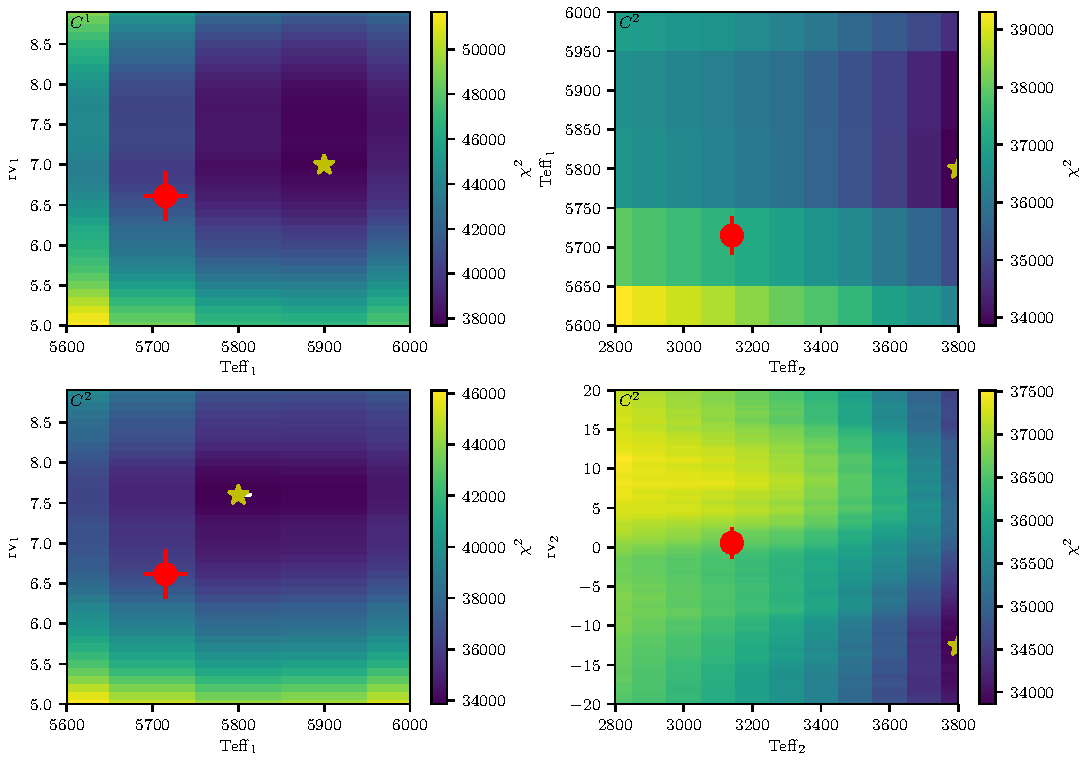
\includegraphics[width=0.7\linewidth]{figures/companion_recovery/HD211847_result_pcolors}
    \caption{\textchisquared{} result grid for observation 2 of {HD 211847}, similar to \cref{fig:Mdwarf_contours,fig:HD211847_simulated_contours}.
    The top right plot shows the application of a single component model (\(C^1\)) while the other three are using a binary model (\(C^2\)).
    Both left hand panels show the distribution of host temperature and host {RV}.\@ The top right panel shows the distribution for host and companion temperature, and the bottom right the companion temperature and radial velocity.
    The red circles indicate the literature values or calculated parameters for the target while the yellow star indicates the minimum \textchisquared{} solution.
    The error bar on the \(\teffsub{1}\) is from the literature while the error bars on \({rv}_1\) and \({rv}_2\) are calculated by propagating the orbital parameter uncertainties though the radial velocity equation.
    The white line shows a 3-\(\sigma\) confidence level about the minimum \textchisquared{} solution grid point, not always visible here due to the large \textchisquared{} values.}
    \label{fig:HD211847_result_contours}
\end{figure*}

\todo{Put error paragraph in a good location}
The error on estimated {RV} values, shown in \cref{fig:HD211847_result_contours}, is calculated by applying the general error propagation formula~\citep{ku_notes_1966} to the RV equation (\cref{eqn:rv2_equation}) and using the errors on the published orbital parameters.
For a function, \(f\), with errors on the inputs \(\delta x\), \(\delta y\) etc., it follows:
\begin{align}
f &= f(x, y, z, \ldots)\\
\delta f &= \sqrt{{\left( \frac{\partial f}{\partial x} \delta x\right)}^2 + {\left(\frac{\partial f}{\partial y} \delta y\right)}^2 + {\left(\frac{\partial f}{\partial z} \delta z\right)}^2 + \ldots}.
\end{align}


\begin{figure*}
    \centering

   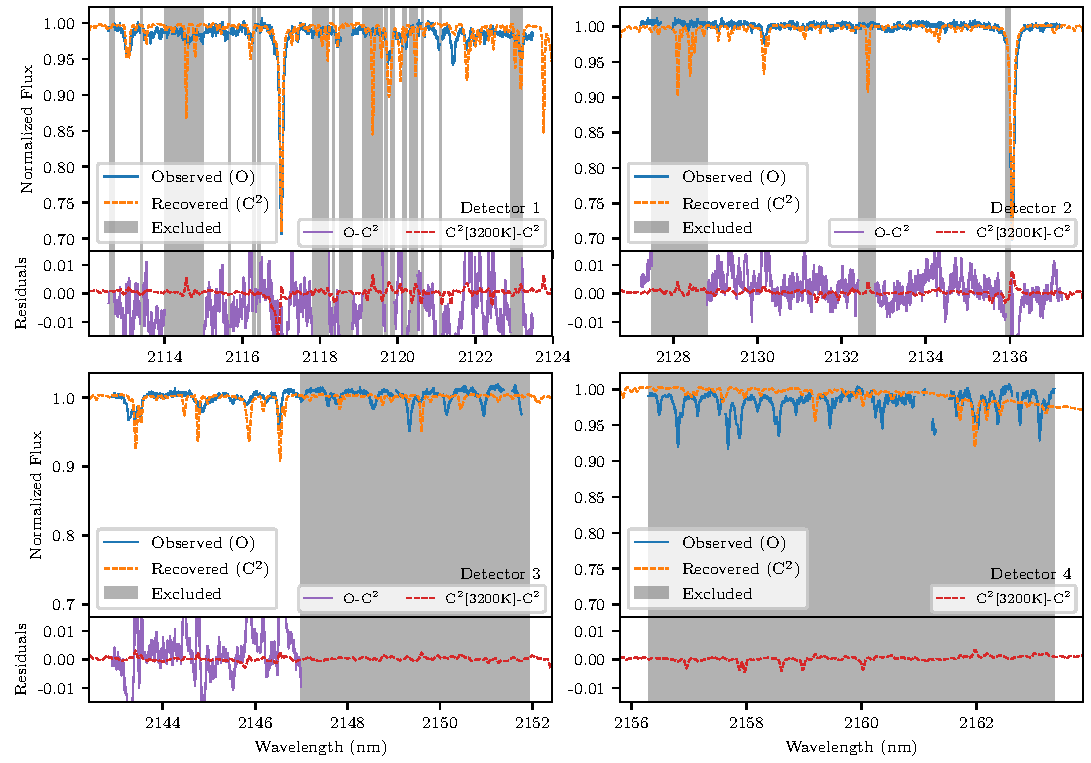
\includegraphics[width=0.7\linewidth]{figures/companion_recovery/visualize_result_residuals}
    \caption{Comparison between the observed {HD 211847} spectrum (blue) and the best fit synthetic binary model (orange dashed) for each detector.
The bottom section of each panel shows the residuals between the parts of the observation used in the \textchisquared{} fit and recovered binary model (\(\rm O-C^2\)) in purple.
The red dashed line shows the difference between the recovered binary model and the binary model with the exact same parameters except for the estimated companion temperature of 3\,200\K{} (\(\rm C^2[3200\K{}]- C^2\)).
The grey shading indicated the wavelength regions where masking has been applied.
The thinner masked regions that match with cuts in the observed spectra are where the centres of deep (>5\%) telluric lines that have been masked out are.}
    \label{fig:visualinspection-hd2118471}
    %\label{fig:visualizeresultresiduals}
\end{figure*}


\subsection{Companion injection-recovery}
\label{subsec:injection-recovery}
To determine the detection limits for this method we employ an injection-recovery approach.
We take the observed spectra and inject onto them a synthetic companion, at the absolute flux ratio to which it would have been added to a synthetic host with the same parameters.
The injected companion {RV} is set to 100\kmps{} so that the companion lines are well separated from the lines of the host.
This separation chosen is slightly larger than what we have with our observations, \(rv_2\) given in \cref{tab:observations}.

We restrict the search space by fixing the host parameters \(\teffsub{1}\) and \(\logg{}_1\) to those recovered fitting the non-injected spectra by a single component model.
The wavelength masking is used to reduce the level of mismatch between synthetic and observed spectra.

We apply the recovery method developed above on the injected spectrum, leaving only the companion \(\teffsub{2}\) and \({rv}_2\) parameters free, to recover the injected companion.
We repeated this for injected companions with temperatures below 5\,000\K{}.

We also perform the injection-recovery with synthetic host spectra, representing each target.
The wavelength range of the synthetic spectra used for this is three sections interpolated to 1\,024 values in the wavelength span of detectors 1, 2, and 3.
For each section, Gaussian noise is added at the level measured in the corresponding detector in the observation of the target being represented.

In \cref{fig:injectrecoveryhd30501} we show the results of the injection-recovery on {HD 30501}.
The blue dots represent the recovered companion temperature when injected into real observations, while the orange triangles represent injection into a synthetic host.
Error bars of \(\pm100\)\K{} are included to indicate the grid size, and do not come from the recovery itself.
The black dashed diagonal is the temperature 1:1 relation, where a correctly recovered companion should lie.

The grey shaded region indicates the \(\pm1\,000\)\K{} temperature range explored for the injection-recovery of the companion.
This shows how the bounds of the grid are recovered at low temperatures.

For {HD 30501} the injection onto synthetic and observed spectra produce similar results.
At temperatures above 3\,800\K{}, in both the real and synthetic spectra, the injected companion is recovered within 100\K{}.
For injected companion temperatures below 3\,800\K{} the temperature recovered is systematically higher than the injected value.
This indicates that the companion is not correctly recovered and is affected by the added noise.
We determine this temperature to be the upper temperature limit for the recovery.
For the other stars we could not conclude on the upper limit due to spectral mismatch issues.
In these cases we use the results from the synthetic injection to derive a temperature recovery cut-off for each target, each simulated with the closest host star spectrum.

In \cref{fig:injection_shape} we show the minimum \textchisquared{} for each companion temperature in the recovery grid.
We do this for 7 different injected companion temperatures between 2\,500 and 4500\K{}.
For the higher temperature companions, the \textchisquared{} is parabolic in shape, recovering the correct temperature, as expected.
At lower temperatures there is a strong asymmetry in the \textchisquared{} with it flattening out on the lower temperature side.
The 1-, 2-, 3-\(\sigma\) values (with 2 degrees of freedom) of 2, 6 and 11 above the minimum \textchisquared{} are not shown in the bottom panel of \cref{fig:injection_shape} which is a close-up around the minimum \textchisquared{} as are indistinguishable in the top panel due to the \textchisquared{} y-scale.
The black vertical line indicates the 2\,300\K{} temperature limit of the {PHOENIX-ACES} models.

\begin{figure}
    \centering
    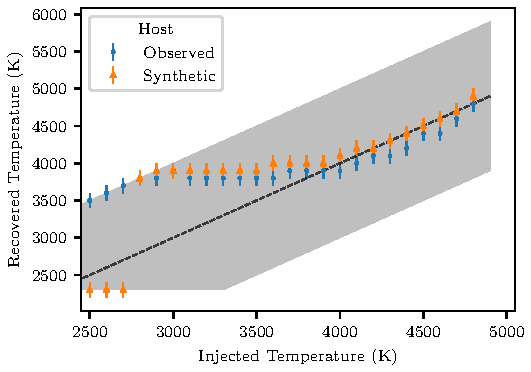
\includegraphics[width=0.6\linewidth]{figures/companion_recovery/inject_recovery_hd30501.pdf}
    \caption{Result of simulated injection-recovery of synthetic companions on {HD 30501}.
    The blue dots and orange triangles indicate the recovered companion temperature for the observed and synthetic spectra respectively.
    The \(\pm100\)\K{} error bars are the grid step of the synthetic models.
    The black dashed diagonal shows the 1:1 temperature relation.
    The grey shaded region indicates the \(\pm1\,000\)\K{} temperature range explored.
    Gaussian noise added to the synthetic spectra was derived from the observed spectra.}
    \label{fig:injectrecoveryhd30501}
\end{figure}


\begin{figure}
    \centering
    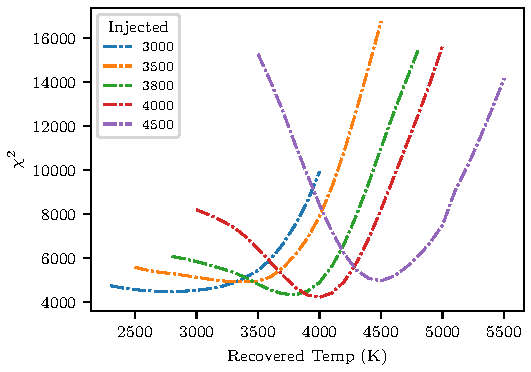
\includegraphics[width=0.7\linewidth]{figures/companion_recovery/chi2_shape_investigation}
    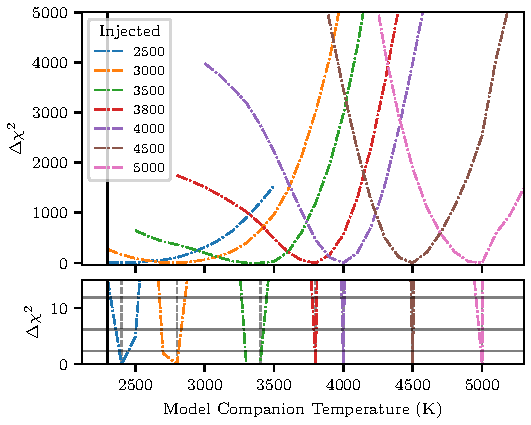
\includegraphics[width=0.7\linewidth]{figures/companion_recovery/chi2_shape_investigation_with_delta}
    \caption{(top) Companion temperature verses \textchisquared{} for simulations with different injected companion temperatures.
    Other fixed parameters for these fully synthetic simulations was \(\teffsub{1}=5\,200\)\K{}, \(\logg_1=4.5\), \(\logg{}_2=5.0\), and both \feh{}=0.0.
    A fixed Gaussian noise corresponding to a \snr{} of 300 was used.
    (bottom) A close up view of \textchisquared{} < 15.
    The three horizontal grey lines indicate the 1-, 2-, 3-$\sigma$ with 2 degrees of freedom.
    The vertical dotted lines indicate the location of the minimum \textchisquared{} recovered for each companion.
    The black solid vertical in both panels shows the 2\,300\K{} cut-off of the {PHOENIX-ACES} models}
    \label{fig:injection_shape}
    %\label{fig:chi2shapeinvestigation}
\end{figure}

%!TEX root = ../thesis.tex
\begin{table}
       \centering
  \begin{threeparttable}

       \caption{Upper mass limits of target companions assuming a companion \logg{}=5.0. Masses are derived from~\citet{baraffe_new_2015} evolutionary models using \(\teff{}\) and \logg{}. The flux ratio \(\rm F_2/F_1\) is  the absolute flux ratio between the cut-off temperature and the target host star.}

        \begin{tabular}{l c c c}
            \toprule
            Target & \txteff{} cut-off (K) & \(\rm F_2/F_1\) & Mass limit (\Mjup{})\\
            \midrule
            {HD 4747}     &  3\,900 & 0.084 & 598 \\
            {HD 162020} & 3\,900 & 0.147 & 598 \\
            {HD 167665} & 3\,800 & 0.054 & 560 \\
            {HD 168443} & 4\,000 & 0.094 & 618 \\
            {HD 202206} & 3\,900 & 0.075 & 598 \\
            {HD 211847} & 3\,900 & 0.079 & 598 \\
            {HD 30501}   & 3\,800\tnote{a} & 0.106 & 560 \\
            \bottomrule
        \end{tabular}
        \label{tab:mass_limits}
        \begin{tablenotes}[flushleft]
            \small
                \item [a] {From observed spectra }
        \end{tablenotes}
  \end{threeparttable}

\end{table}



Using the temperature cut-off values, we derive an upper mass limit for the companions around our stars using the~\citet{baraffe_new_2015} evolutionary models, finding the closest point matching the spectral temperature cut-off and \(\logg{}=5.0\).
These values are given in \cref{tab:mass_limits} and are between 560 and 618~\Mjup{}.
The flux ratio between the cut-off and the host star are also provided for, being between 5 and 15\% in this wavelength span.




% DISCUSSION



\citet{hoeijmakers_search_2015}
{Context.
The spectral signature of an exoplanet can be separated from the spectrum of its host star using high-resolution spectroscopy.
During these observations, the radial component of the planet's orbital velocity changes, resulting in a significant Doppler shift that allows its spectral features to be extracted. \\
     Aims: In this work, we aim to detect\ce{TiO} in the optical transmission spectrum of HD 209458b.
Gaseous\ce{TiO} has been suggested as the cause of the thermal inversion layer invoked to explain the dayside spectrum of this planet. \\
     Methods: We used archival data from the 8.2 m Subaru telescope taken with the High Dispersion Spectrograph of a transit of HD 209458b in 2002.
We created model transmission spectra that include absorption by\ce{TiO}, and cross-correlated them with the residual spectral data after removal of the dominating stellar absorption features.
We subsequently co-added the correlation signal in time, taking the change in Doppler shift due to the orbit of the planet into account. \\
     Results: We detect no significant cross-correlation signal due to\ce{TiO}, though artificial injection of our template spectra into the data indicates a sensitivity down to a volume-mixing ratio of \textasciitilde{}10\textsuperscript{-10}.
However, cross-correlating the template spectra with a {HARPS} spectrum of Barnard's star yields only a weak wavelength-dependent correlation, even though Barnard's star is an M4V dwarf that exhibits clear \ce{TiO} absorption.
We infer that the\ce{TiO} line list poorly matches the real positions of\ce{TiO} lines at spectral resolutions of \textasciitilde{}100 000.
Similar line lists are also used in the {PHOENIX} and Kurucz stellar atmosphere suites and we show that their synthetic M-dwarf spectra also correlate poorly with the {HARPS} spectra of Barnard's star and five other M dwarfs.
We conclude that the lack of an accurate\ce{TiO} line list is currently critically hampering this high-resolution retrieval technique.},




\subsection{Junk from paper about BT-settl}

The {PHOENIX-ACES} models also provide dimensions of effective radius of the star, in the header.
This is required for the method presented here as we need to scale the spectra by their respective surface area when combining together.


The effective radius of the modelled star are provided in the fits header and required for the calculation of the flux ratio.


As we do not recover suitable results for HD211847 which is supposed to have a temperature around 3\,400\K{} we suspect that it is not possible for lower temperature either so don't try to extend to the {BT-Settl} models.


\textbf{
     {PHOENIX-ACES}  defines grid as Teff,\logg{} and Mass which can then be used to determine Radii.
See~\citep{husser_new_2013} section 2.3.1 Mass.}





\subsection{Incremental changes}
\textbf{incremental changes in models are small}

We took the synthetic models and investigated how the synthetic binary changed as the model parameters were incremented.
For the temperature of the companion to be incremented by 100\K{} this resulted in change to the spectrum with a standard deviation of \textbf{XXX}.
This is around a \snr{} of around 500.
The change in the models with incremental changes in temperature is small, Changes in \logg{} and \feh{} are larger but we fixed these for the application above.





\subsection{Note about a target - discussion of results}
Another example is \object{HD 162020}, which has the lowest orbital period (8.4 days) of our targets.
It should have been possible to obtain an optimal pair of observations in one semester, but the second observation was taken immediately following the first.
This means that the \(\rm \delta {RV} = 0.363\kmps{}\)between the two observations, is comparable to the \(\Delta {RV}\)that occurs during each individual observation.
With tighter scheduling restrictions this target could have been observed with the optimal {RV} separation at the extrema of \(\Delta {RV}=2 K_{2}\).
Whether the flux ratio of \(7e^{-6}\) for this target and the interaction of different spectral lines would have made it possible to recover companion mass is a separate issue.



\subsubsection{Wavelength range}
The wavelength choice for the spectra analysed here, observed with the intention to apply the spectral differential technique, was selected due to the location of the \emph{K}-band telluric absorption window.
This wavelength range, with a narrow wavelength range \(\sim50\)\nm{} set by the {CRIRES} instrument.
This wavelength range is likely not the best choice for the proposed study. \todo{finish this line} may contribute to the poor results from the companion recovery technique.

For instance~\citet{passegger_fundamental_2016} used four different spectral regions for the precise parameter determination of M-dwarfs.
Specific lines from the different wavelength regions are affected differently by the model parameters: \(\teff{}\), \logg{}, and \feh{}; and are used to break degeneracies in the {PHOENIX-ACES} parameter space.

Changing the wavelength coverage to regions with lines sensitive to stellar parameters for both stars and BDs, as well as using a larger wavelength range that will be achieved by {CRIRES+}, may help to improve the recovery results of the companion recovery technique presented here.
We note that if the wavelength range is increased by taking separate observations at different wavelengths, not covered by a single exposure, then changes in the {RV} of both components between the different wavelength observations may need to be accounted for.



\subsection{Comparison to other methods}
kolbl 2014,  passenger 2016, 2018




\section{Summary}

	
	%!TEX root = ../thesis.tex
% NIR-information

\chapter{Information content of \nir{} Spectra}
\label{cha:nir_content}

The work presented in this chapter focuses on calculating and analysing the information content of stellar spectra ,specifically the radial velocity precision in the \nir{}. \todo{this doesn't seem right}{It is very different from the previous chapters in which the detection of the companions spectra was attempted.}

The field of exoplanet detection in the \nir{} is expanding with several new high resolution \nir{} spectrographs available in the near future. For instance {CARMENES} is already performing observations while SPIRou, {NIRPS}, and CRIRES+ are near completion. One science objective common to all four instruments is the detection small mass planets around {M-dwarf} stars utilizing the radial velocity technique.
The fundamental radial velocity precision of {M-dwarf} spectra attainable at different wavelength regions calculated in \citet{figueira_radial_2016} was used to influence some design choices of SPIRou, {NIRPS} specifically.

The purpose of the work presented in this chapter is to extend the work of \citet{figueira_radial_2016}, computing the theoretical RV precision of stellar spectra over a wider range of situations. A investigation into the effect of \logg{} and \feh{} on precision is performed and a comparison of RV precision of he recently observed \nir{} {M-dwarf} spectra from {CARMENES} library and their synthetic counterparts will be performed. This is to test how the {RV} precision of synthetic models compares to reality.
The aim is to compare the fundamental precision of \nir{} spectra to the synthetic models, to


\section{Overview}

The pursuit of detecting exoplanets, especially ``habitable'' and ``Earth-like'' planets, requires state-of-the-art instrumentation with high precision. One of the key detection methods, the Radial Velocity ({RV}) method, measures the wobble induced on the Star by the planet as they orbit their common barycentre \reference{rv method}.  {\red{} add Some stuff about mass and period from Pedros paper}  \todo{put in introduction??}



A increase in the number of \nir{} spectrographs is increasing to focus on cooler {M-dwarfs} stars which have a easier* chance of detecting Earth-like planets in the habitable zone. \change{Check mission statements for these}{SPIRou, {NIRPS}} and {CARMENES}. Also {CRIRES+}\ldots{}
This work continues the assessment of {RV} precision levels possible in this domain.
\todo{For example from Figueira 2016 see figure} A more precise measurement can be achieved from X band then the \emph{Y}-band\ldots{} or in order XYZ of precision.

\missingfigure{An example from Figueira et al. 2016}



This work is not directly related to detecting exoplanet atmospheres themselves but investigates the theoretical and observed {RV} precision of {M-dwarf} spectra in the \nir{}. This has previously helped the aid the direction of instrument design by identifying the wavelength regions with the best {RV} precision~\citep{figueira_radial_2016} but can also help in the planning of observations, by understanding how the precision changes with spectral type and observed {SNR}. This can help in detecting the presence of ``habitable Earth-like'' planets around {M-dwarfs} which will likely have their atmospheres eventually probed.


\section{Radial velocity precision}
The first detections of extrasolar planets with the {RV} technique were hot-Jupiters; Jupiter mass planets in close orbits to their star . The RV precision required to detector the first hot-Jupiter, 51 Peg b, was \todo{find mayor queloz precision achieved} \cite{mayor_jupitermass_1995} using \todo{what reference} Since that time the instrumental development and the detection and observations technique refined to achieve {RV} precisions better than 1\mps{}. The recently commissioned ESPRESSO optical spectrograph is designed with the goal of achieving 10\cmps{}. The level of precision required to detect an Earth mass planet in an 1 year orbit round a Sun-like star.

Over the years the community has push the limits of this technique to smaller and smaller planetary masses. An example is shown in \fref{fig:year_mass}.

\begin{figure}
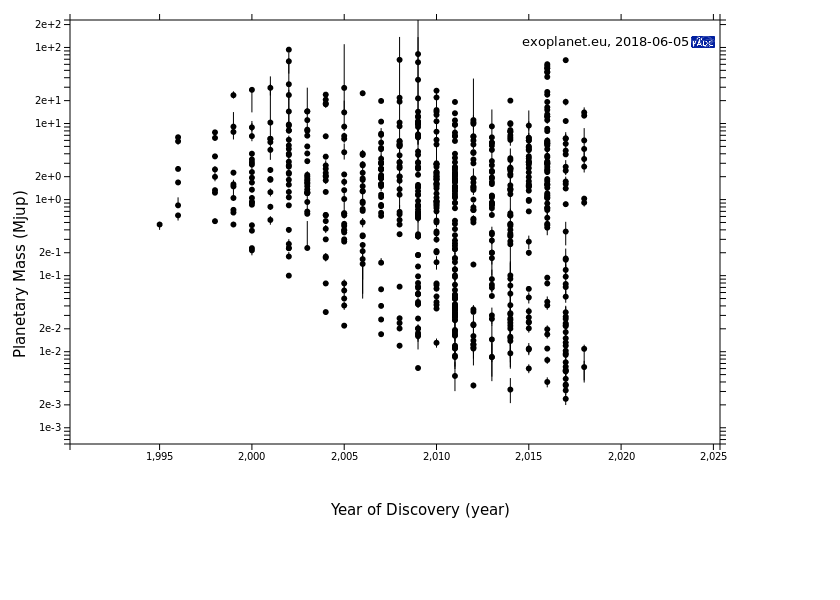
\includegraphics[width=0.8\linewidth]{figures/year_planet_mass.png}
\caption{Mass of discovered planets verse year. From Exoplanet.eu}
\label{fig:year_mass}
\end{figure}


{RV} amplitude scales with mass of the star \({M_{\star}}^{-2/3}\) and with the planetary orbital period \({P_{\textrm{orb}}}^{-2/3}\).

The detection of an Earth-mass planet inside the habitable zone around a solar-type star, the {RV} amplitude is 10 \cmps{}. If that a planet with the same characteristics is instead orbiting a {M-dwarf}, the {RV} amplitude is larger than 1\mps{}. This is due to two factors, the smaller mass of the host star, and the closer habitable zone, due to a lower luminosity output of the host.

\citet{artigau_optical_2018} recently compared archival spectra of Barnard's Star, an {M-dwarf}, and found that state-of-the-art atmosphere models over-predict the \emph{Y}- and \emph{J}-band {RV} content by more than a factor of \(\sim 2\), while under-predicting the \emph{H} and \emph{K}-band content by half.
{\red{} in this work we find similar?}

We are currently aiming to extend this work over the whole {M-dwarf} range, from {M0}-{M9}.

\todo{History of Precision calculations}
History of Precision calculations:
Connes 1\,985 -
Bouchy et al. 2001  - photon noise limit on rv measurements.
\cite{figueira_radial_2016} - focus on {M-dwarfs} parameter range to specify new instrumentation windows to focus.
Reiners 2017 -  {CARMENES} sample. Some precision
pedros school section other precision source \({r}^{1.5}\)


\subsection{Fundamental photon noise limitation}
\label{fundamental_precision}
A technique to calculate the theoretical radial velocity precision of a spectrum using the full spectral information in an optimal way was presented by~\citet{connes_absolute_1985}. Here we provide the radial velocity precision derivation following~\citet{connes_absolute_1985, bouchy_fundamental_2001, figueira_radial_2016}. A majority of this derivation follows~\citet{bouchy_fundamental_2001} with extra explanations and notes added.

\begin{figure}
    \centering
    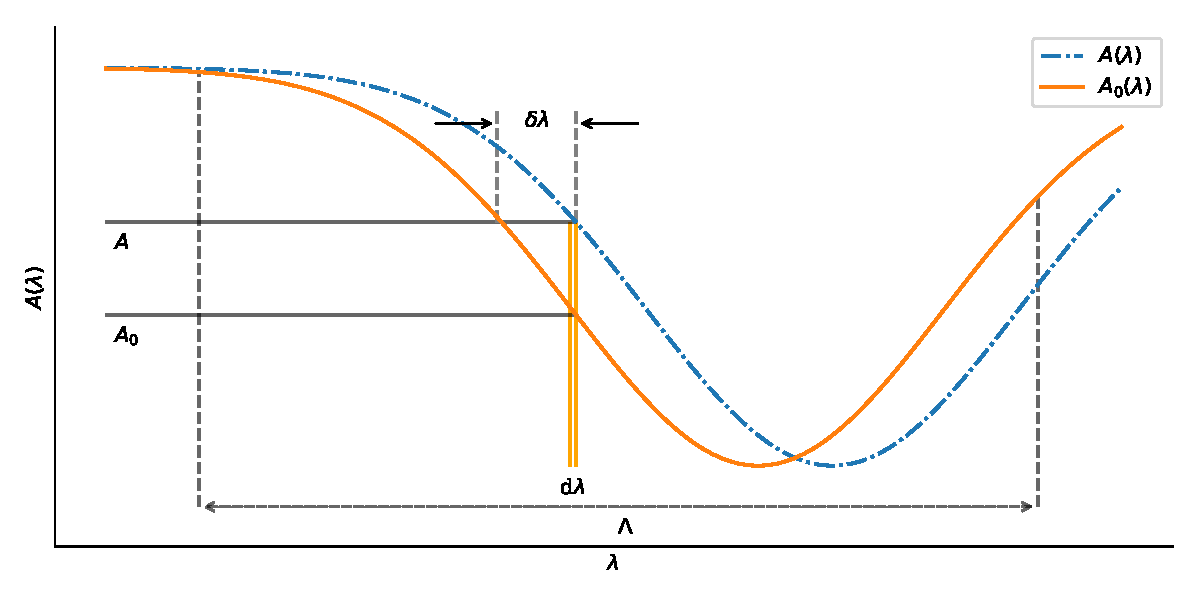
\includegraphics[width=0.7\linewidth]{figures/information-content/precision_plot.pdf}
    \caption{Arbitrary spectral line with a shift \(\delta \lambda\), inspired by~\citet{connes_absolute_1985}.  \(\Lambda\) is the wavelength range considered.}
    \label{fig:precisionderivation}
\end{figure}
\todo{add \(\delta A\) to plots}

For demonstration purposes  \fref{fig:precisionderivation} show a portion of an arbitrary spectrum \(A(\lambda)\), for demonstration purposes over a wavelength range \(\Lambda\). Here \(A_0(\lambda)\) is the reference spectrum while \(A(\lambda)\) is observed some later time with an apparent wavelength shift observed. It shows most of a single Gaussian line as spectral lines contain the most information but the requirement of spectral lines is not a requirement.

The Doppler shift of a spectrum is given by:
\begin{equation}
\frac{\delta V}{c} = \frac{\delta \lambda}{\lambda},
\label{eq:dopplershift}
\end{equation}
where \(c\) is the speed of light in a vacuum, and \(\delta \lambda\) is the shift in wavelength \(\lambda\) due to the velocity \(\delta V\).

\todo{intensity change from connes is vertically in the slice d lambda}

Using basic calculus \(\delta y = \pd{y}{x} \delta x \nonumber\), and for a Doppler shift that is small compared to the line-width\footnote{Although~\citet{connes_absolute_1985} show that the approximation in \eref{eq:intensitychange} is adequate under all circumstances}, the observable intensity change in a wavelength slice \(d \lambda\) (or at a given pixel) can be expressed by:

\begin{equation}
\delta A(i) = A(i) - A_0(i) \simeq \pd{A_0(i)}{\lambda(i)} \delta \lambda
\label{eq:intensitychange}
\end{equation}

Rearranging \eref{eq:intensitychange} for \(\delta \lambda\) and combining it with \eref{eq:dopplershift}, the Doppler shift of then becomes:
\begin{equation}
    \frac{\delta V(i)}{c} = \frac{A(i) - A_0(i) }{\lambda(i) (\partial A_0(i)/\partial \lambda(i))} \label{eq:delta_v_i}
\end{equation}

This equation shows that the radial velocity measured at pixel, i, through a change in the intensity in the recorded spectrum, \(A(i)-A_0(i)\), and inversely proportional to the slope of the spectrum, \({\partial A_0(i)}/{\partial \lambda(i)}\).
\ref{eq:delta_v_i} provides a separate measurement of the radial velocity shift for every pixel, $i$, in the spectrum. The sensitivity of the velocity measurement can be improved, and the noise decreased by using the information from the whole  spectral range, \(\Lambda\). This is achieved by taking the weighted average\footnote{Weighted average on x is \(\bar{x} = \frac{\sum{ x(i)W(i)}}{\sum {W(i)}}\)} over all pixels in the spectral range using an optimal pixel weight \(W(i)\).

\begin{equation}
\bar{\frac{\delta V}{c}} = \frac{\sum{\frac{\delta V(i)}{c}W(i)}}{\sum {W(i)}}.
\end{equation}

Statistically, the optimal weights are proportional to the inverse square of the individual dispersion (variance),

\begin{equation}
W(i) = \frac{1}{{\left(\frac{\delta V_{\rms}(i)}{c}\right)}^{2}}, \label{eq:weights}
\end{equation}
where \(X_{\rms}\) is the dispersion on the quantity \(X\).


The individual dispersion of the velocity measurement \(\delta V_{\rms}(i)\) is the dispersion that would result from several measurements of the reference spectrum all with the same Doppler shift (e.g.\ zero). \eref{eq:delta_v_i} thus becomes:
\begin{equation}
    \frac{\delta V_{\rms}(i)}{c} = \frac{{[A(i) - A_0(i)]}_{\rms} }{\lambda(i) (\partial A_0(i)/\partial \lambda(i))}. \label{eq:delta_v_i_rms}
\end{equation}
The noise of the spectrum A is the quadratic sum of the photon noise \(\sqrt{A}\) and the detector noise \(\sigma_D\). The spectrum \(A_0\) is considered noise free.

\begin{equation}
{[{A(i)-A_0(i)}]}_{\rms} = {[{A(i)} - 0]}_{\rms} = \sqrt{{\sqrt{A(i)}}^{2} + {{\sigma}^{2}}_{D}} \label{eq:noise}
\end{equation}
Considering that the Doppler shift is small and that \(A\) and \(A_0\) have the same intensity level, then \(A = A_0\) can be set. Using Equations~\ref{eq:delta_v_i},~\ref{eq:weights}, and~\ref{eq:noise} the optimum weights then become solely dependent on the reference spectrum.

\begin{equation}
W(i) = \frac{{\lambda}^{2}(i) {({\partial A_0(i)}/{\partial \lambda(i)})}^{2}}{A(i) + {\sigma}^{2}_{D}} \label{eq:optimal_weight}
\end{equation}

This weighting function can be modified to mask out and eliminate unwanted lines in the spectrum. For instance in the removal of telluric absorption lines in observed spectra. This is achieved to setting the particular pixel weights to zero.

With the optimal weights set, the weighed average velocity change measured from the full spectral range \(\Lambda\), is given by:

\begin{eqnarray}
    \frac{\overline{\delta V}}{c} &= \frac{
        \sum{
            \frac{
                A(i) - A_0(i)}{
                \lambda(i) \left({\partial A_0(i)}/{\partial \lambda(i)}\right)} W(i)}}{
             \sum{{W(i)}}} \\
    &= \frac{
        \sum {
            (\frac
                {A(i) - A_0(i)}
                {\lambda(i) (\partial A_0(i)/\partial \lambda(i))}) \frac
                    {{\lambda}^{2}(i) {({\partial A_0(i)}/{\partial \lambda(i)})}^{2}}
                    {A_{0}(i) + {\sigma}^{2}_{D}}
                 }
         }
    {\frac
        {{\lambda}^{2}(i) {({\partial A_0(i)}/{\partial \lambda(i)})}^{2}}{A_{0}(i) + {{\sigma}^{2}}_{D}}
        } \\
    &= \\
    &= \frac{\sum{(A(i) - A_0(i)){\left(\frac{W(i)}{A_0 +{\sigma}_{D}^{2}}\right)}^{1/2}}}{\sum{W(i)}}
    \label{eq:delta_v_eqarray}
\end{eqnarray}\unfinished{Finish this equation (9 of bouchy 2001)}
\unfinished{Try the symbolic package from PC}

The important quantity for {RV} measurements is not just the velocity values themselves but also the dispersion on the measured velocity, the RV precision, \(\delta V_{\rms}\), from the spectrum. This allows one to assess the planetary detectability limitations attainable in the spectra. From rearranging \eref{eq:weights} the dispersion is given by:

\begin{equation}
    \overline{\frac{\delta V_{\rms}}{c}} = \frac{1}{\sqrt{\sum{\,W(i)}}} = \frac{1}{Q \sqrt{\sum{\,A_0(i)}}}. \label{eq:dv_rms}
\end{equation}
With this the velocity precision is inversely proportional to the sum of the optimal pixel weights.

A spectral quality factor, Q, is defined as for the pure photon noise case in~\cite{connes_absolute_1985, connes_demonstration_1996}, as:
\begin{equation}
Q = \frac{\sqrt{\sum{\,W(i)}}}{\sqrt{\sum{\,A_0(i)}}}.
\end{equation}

The radial velocity precision or uncertainty can be rearranged in terms of the spectral quality;

\begin{equation}
    \delta V_{\rms} = \frac{c}{Q \sqrt{\sum {\,A_0(i)}}} = \frac{c}{Q \sqrt{{N}_{{e}^{-}}}} \approx \frac{c}{Q (S/N)},
\end{equation}

where \(\sum A_0(i) = {N}_{{e}^{-}}\) is considered to be the total number of photo-electrons \({N}_{{e}^{-}}\) counted in the spectral range considered.\todo{explain snr}{where the \({SNR}=\sqrt{N_{{e}^{-}}}\)for large N}
where the \({SNR}=\sqrt{N_{{e}^{-}}}\)for large N. \unfinished{It is convenient to use this version when comparing observed spectra with different S/N.?}


This quality factor, Q, is flux independent and is purely a function of the spectral profile within the spectral range considered. It is a measure of the line richness i.e., quantity and depth. For example a spectrum with many sharp lines will have a high Q. This quality factor is valid for the pure photon noise case only in which \(\sigma_{D} =0\) and \({[A(i)]}_{\rms} = A_0\). The instrumental resolution of the spectrograph also effects the spectral quality as it induces line broadening.

The number of photo-electrons counted \(N_{{e}^{-}}\) depends on the stellar magnitude, detector efficiency and integration time. It can be estimated using
 \begin{equation}
 N_{{e}^{-}} = P_{avg} * S_{tel} * T_{\textrm{exp}} * \alpha* \Lambda,
 \end{equation}

where \(P_{avg}\) is the average monochromatic stellar brightness
across the wavelength range \(\Lambda\) in \si{\photons\per\second\per\centi\metre\squared\per\centi\metre},
\(S_{tel}\) is the telescope collecting area in \si{\centi\metre\squared},
\(T_{\textrm{exp}}\) is the integration time in \si{\second},

and \(\alpha\) the overall efficiency (including atmosphere, telescope, spectrograph and detector).

This can be used to determine the {RV} precision for a given instrument, and be useful in exposure time calculators for planning observations for RV surveys and exoplanet detection.

In the case of several \(\delta V\) measurements computed for \(k\) spectral slices (or spectral orders) then the error on the average \(\overline{\delta V}\) is given by the error on a weighted average:
\begin{equation}
\overline{\delta {V}_{\rms}} = \frac{1}{\sqrt{\sum_k{{(\frac{1}{\delta V_{\rms}(k)})}^{2}}}}
\end{equation}


This work follows~\cite{figueira_radial_2016} by exclusively considering a high signal-to-noise regime in which \(A(i) + \sigma_{D}^{2} \sim A(i)\) can be approximated.


\footnote{pure detector noise the fluctuation are independent of the spectrum \(A\) and the quality factor for pure detector noise is \(Q_D = \frac{\sum{{\lambda}^{2} {(\partial A_0(i)/\partial \lambda(i))}^{2}}}{\sum{\, A_0(i)}}\) as derived by~\cite{connes_absolute_1985}. }


This technique has been tested and demonstrated on observations by~\citet{connes_demonstration_1996} and been used to determine predict the accuracy or performance limits of spectrograph instrumentation \citep[e.g.][]{connes_absolute_1985,bouchy_fundamental_2001} and can influence the design (and/or use) of spectrographs
 (e.g.\ SPIROU~\citep{artigau_spirou_2014,figueira_radial_2016})
\unfinished{Does spectrograph pipelines such as HARPS use these equations to measure estimate/precision?}


Considering that \(\sum{A_0(i)} = N_{{e}^{-}}\)is the total number of photoelectrons counted over the whole spectral range then the uncertainty in the velocity change is finally given by:

\begin{equation}
\delta V_{\rms} = \frac{c}{Q \sqrt{N_{{e}^{-}}}} \approx \frac{c}{Q (S/N)}, \label{eq:rv_SNR}
\end{equation}

where the \({SNR}=\sqrt{N_{{e}^{-}}}\)for large N. \unfinished{It is convenient to use this version when comparing observed spectra with different S/N.?}


In the unrealistic case where all the pixel weights are identical $W(i)=w$, then we can also see that the precision with decreases as $1/\sqrt{N}$ due to an increase in the number of pixels, or a increase in spectral range.
 \begin{equation}
 \delta V_{\rms} = \frac{c}{\sum{W(i)}} \approx \frac{c}{\sqrt{N w}}=  \frac{c}{\sqrt{N}\sqrt{w}}, \label{eq:sqrtN}
 \end{equation}


A separate general formula for RV precision is given by \citet{hatzes_spectrograph_1992} in terms of general spectral parameters.
\begin{equation}
\sigma = \frac{1}{\sqrt{F} \sqrt{\Lambda} {R}^{1.5}}
\end{equation}

Here the $\sqrt{F}$ represents the SNR of the spectrum in the possion-noise dominated regime. The $\Lambda$ comes from assuming a homogenous distribution of line, with the same line properties, per unit length.


The 1.5 factor. ....

\subsubsection{summarize}
Summarize the derivation

\subsection{Prepare phoenix aces models}:
\# see~\citet{figueira_radial_2016}

Convert SED to counts.


Scale to 100 \snr{} per resolution element in \emph{J}-band.

Convolutions

\subsection{Rotation convolution}
Stellar rotation has the affect of broadening spectral lines as the different portions of the stellar surface have a variation of radial velocity between \(\pm v \sin i\).
Rotation is applied to a non-rotating spectrum by convolution with a rotation kernel.
The stellar rotational kernel used is given by~\citet{gray_observation_2005};

\todo{top view diagram of rotation?}

\begin{align}
G(\Delta\lambda) &= \frac{2(1-\epsilon){[1-{(\Delta\lambda /{\Delta\lambda}_{L})}^{2}]}^{1/2} +   \frac{1}{2}\pi\epsilon[1-{(\Delta\lambda /{\Delta\lambda}_{L})}^{2}]}{\pi (1-\epsilon/3)\vsini}\\
      &= c_{1}{[1- {(\Delta\lambda /\Delta\lambda_{L})}^{2}]}^{1/2} + c_{2}[1-{(\Delta\lambda /\Delta\lambda_{L})}^{2}] \label{eqn:rotational_profile}
\end{align}
where
\begin{equation}
c_1 = \frac{2(1-\epsilon)} {\pi (1-\epsilon/3)\vsini},  \hspace{4em} c_2 = \frac{\frac{1}{2}\pi\epsilon} {\pi (1-\epsilon/3)\vsini},
\end{equation}
are constants which depend on the equatorial rotational velocity \(\vsini\).

Here $\Delta\lambda$ is the wavelength position from the non-rotating line centre, $\Delta\lambda_{L}$ is the maximum line shift of the line centre at the edge of the stellar disk at which point the Doppler shift is  \(\vsini\); $\Delta\lambda_{L} = \lambda \frac{\vsini}{c}$.

This kernel arises from integrating the rotational velocity profile across the surface of the stellar disk and as such the rotation kernel is bounded in the range  $[-\Delta\lambda_L, \Delta\lambda_{L}]$ from the line centre.
This kernel also accounts for limb-darkening on the stellar disk with the linear limb darkening coefficient used in this work fixed at $\epsilon=0.6$ as done in \citet{figueira_radial_2016}.

Since the synthetic models do not have a consistent wavelength grid, the discretization of applying the convolution kernel onto the changing wavelength grid causes the result of each pixel to be multiplied by a slightly different kernel area.
Therefore, the result is divided by a convolution of a spectrum of ones with the same wavelength resolution to normalize the convolution.

As the Doppler shift \(\vsini\) is transformed into wavelength by multiplication of $\lambda  / c$ there is a wavelength dependence on the rotation kernel shape. That is, the rotation kernel at each pixel is unique and requires separate calculation. For small wavelength ranges this can be held fixed to improve performance. This simplifications is not performed in this work as large wavelength ranges are considered.


\subsection{Instrumental Convolution}
Following the rotational convolution the spectra are convolved with Gaussian instrumental profile ({\textrm{IP}}) with the {\fwhm}  constrained by the spectral resolution R, $\fwhm= \lambda/R$.

The Gaussian convolution kernel is of the form
\begin{equation}
IP(\Delta\lambda) = \frac{1}{\sigma \sqrt{2\pi}} \exp^{-\frac{{\Delta\lambda}^{2}}{2 {\sigma}^{2}}}    \label{eqn:IP_profile}
\end{equation}

with $\sigma = \frac{\fwhm}{2\sqrt{2 \ln(2)}}$, and $\Delta \lambda$ again the difference from the line centre (normally this would be written as $(x-\mu)$ where $\mu$ is the Gaussian centre).

This assumes that the instrument profile of a particular instrument is in-fact Gaussian. This assumption of a Gaussian instrumental profile is a good starting point for high-resolution spectrographs, and shown to be valid for CRIRES \citep{seifahrt_synthesising_2010}.
If the instrument profile of a particular instrument is well characterized, then it could replace the Gaussian profile used here.

For instance \citet{artigau_optical_2018}  state that the instrumental profile of a (circular) fibre-fed spectrograph such as {HARPS} is mathematically equivalent to a cosine between $\frac{-pi}{2}$ and $\frac{pi}{2}$ with a width equivalent to the Gaussian {\fwhm}.

The integration of a circular fibre is given by
\begin{equation}
\textrm{IP}_{\textrm{fibre}(\Delta\lambda)} = \cos(B\cdot\Delta\lambda) ,  \hspace{2em} [-pi/2B, pi/2B]
\end{equation}
where \todo{define fwhm0}{$B = \frac{\fwhm_{0}}{\fwhm}$ } is a scales to give the same area? \todo{CHECKTHISRESUSLT!!!!!!}
following the description from \citet{artigau_optical_2018}.  They also mention that the result using this $\textrm{IP}_{\textrm{fibre}}$ are all consistent with the Gaussian kernel.

\subsection{Numerical Convolution}
\label{subsec:numerical_convolution}
In this work the stellar models undergo broadening by convolution with rotation and instrumental profile kernels (Equations~\ref{eqn:rotational_profile} and~\ref{eqn:IP_profile}).
The convolutions are performed by analysing a single pixel at a time, and selecting the neighbouring pixels that fall within the convolution window\footnote{Region in which the convolution kernel will affect this particular pixel} for that pixel.
The value of the convolution kernel is calculated at the position of each pixel selected, multiplied by the flux of each pixel and then summed to provide the new value at the selected single pixel{$^{\textbf{*}}$}.
 The shape of the convolution kernels and the size of convolution window are wavelength dependant (${\fwhm}=\lambda / R$ and $\Delta\lambda_{L}=\lambda \frac{\vsini}{c}$) and must be calculated separately for each pixel, making the convolution computationally expensive.

 However, the computation of the convolution of individual pixels is an ``embarrassingly parallel''\footnote{\href{https://en.wikipedia.org/wiki/Embarrassingly\_parallel}{https://en.wikipedia.org/wiki/Embarrassingly\_parallel}} problem.
 What this means is that convolution result for pixel $i+1$ does not depend on the convolution result obtained for pixel $i$.
 Therefore, parallel processing was implemented to improve the performance of the convolution, roughly dividing the convolution time by the number of processors used.

The python package \emph{PyAstronomy} also contains functions that perform rotational and instrumental broadening. Those functions however require that the spectrum have uniformly spaced $x$-coordinate spacing which is not a requirement for the implementation of \emph{eniric} used here. \emph{PyAstronomy}, while implemented a ``slow'' full version of the rotational convolution, with a wavelength dependent kernel, they also provide ``fast'' convolution kernels that are fixed, taking the central wavelength value. These are significantly faster but are only valid for very short wavelength regions, in which the kernels do not significantly change. They are not suitable for use in this work due to the large wavelength span of spectroscopic bands and the wavelength dependant spacing of the spectra. A comparison of the performance between \emph{PyAstronomy} convolution and the convolutions implemented in \emph{eniric} and used here are given in a \emph{Jupyter} notebook in the repository of ``eniric'', basically they fall in between the ``fast'' and ``slow'' implementation of \emph{PyAstronomy}.

One factor the needs consideration when convolving with an non-uniformly spaced spectrum is effect of the sampling on the convolution.
For instance the number of point inside the convolution, as well as their location will effect the area of the convolution kernel.
To normalize the convolution result it is divided by the convolution of a unitary spectrum of ones, with the same spacing.
\citet{figueira_radial_2016} performed this unitary convolution separately and applied the normalization afterwards.
In the improved implementation the convolution normalization is performed directly after the convolution kernel multiplication at \(\textbf{*}\).

For example for the rotational convolution result of the value for pixel $i$ becomes
\[{A}^{\prime}(\lambda_{i}) =  \frac{\sum A(\Delta\lambda_{i}) \cdot G(\Delta\lambda_{i})}{\sum G(\Delta\lambda_{i})},\]
where $\Delta\lambda_{i}$ are the values between in the range $\lambda_{i} (1-\frac{\vsini}{c}) \le\lambda_{i} \le \lambda_{i} (1+ \frac{\vsini}{c})$,
instead of only
\[{A}^{\prime}(\lambda_{i}) =  \sum A(\Delta\lambda_{i}) \cdot G(\Delta\lambda_{i}).\]


By default edge effects are avoided by providing an input spectra sufficiently wider than the desired output spectrum to prevent edge effects on the portion of the spectrum desired. Since two convolutions are preformed one after the other the original input spectrum is selected wider than needed so that no edge effects will be present after both  addition of  rotation and instrumental broadening by $\vsini$ and R.

%-----------------------------------
%    SUBSECTION 2
%-----------------------------------
\section{}
Preparation of {CARMENES} spectra.


\missingfigure{Example of {CARMENES} spectra before and after correction}

\subsection{Bands}
The bands are selected based on the strong water absorption. This can be seen the {CARMENES} spectra in Figure~\reference{Add figure here}\todo{Add figure here}. The wavelength ranges used in this work~\citet{figueira_radial_2016} and used in this work are given in \tref{tab:band_ranges}.
\begin{table}
    \centering
    \caption{The wavelength ranges of the \nir{} spectral bands.}
    \begin{tabular}{cc}
        \toprule
        Band & Range (\um{})\\
        \midrule
        Z & 0.83 -- 0.93\\
        Y & 1.00 -- 1.10\\
        J & 1.17 -- 1.33\\
        H & 1.50 -- 1.75\\
        K & 2.07 -- 2.35\\
        \bottomrule
    \end{tabular}
    \label{tab:band_ranges}
\end{table}



\subsection{Comparing models to {CARMENES}.}
Already somewhat done in Reiners. (use all spectra). They measured the precision obtained in the spectra.

Band by band like \citet{figueira_radial_2016}?
Certain\% steps like Bouchy or Artigau


Can do Barnard's star in {CARMENES}. \todo{finish this} compared to models in Artigau.

\DTLsetseparator{,}
\DTLloadrawdb{targets}{data/carmenes_selection.csv}%

\begin{table*}[h]
    \centering
    \caption{CARMENES library target selection spanning the {M-dwarf} spectral range.}
    \begin{tabular}{l l l r c c c c}%
        \toprule
        Karmn & Name & SpT &  \(\textrm{SNR}_{\textrm{NIR}}\)  & Temp (K) &\logg{} & \feh{} & v\(\sin{i}\) (\kmps{})\\
        \midrule
        \DTLforeach*{targets}{\id=Karmn,\name=Name,\sptype=SpT,\SNR=NIR-SNR,\TEFF=Teff, \LOGG=logg,\metal=FeH, \rot=ROT-Vsini}{
            \DTLiffirstrow{}{\\}\id{} & \name{} &\sptype{} & \SNR{} & \TEFF{} & \LOGG{} & \metal{} & \rot{}
        }
        \\
        \bottomrule
    \end{tabular}
    \label{tab:targets}
\end{table*}

%!TEX root = ../thesis.tex

\begin{table}[h]
    \caption{csv2tex table}
    \begin{tabular}{lllrrrrr}
        \toprule
        Karmn &            Name &   SpT &  NIR-SNR &    Teff &  logg &   FeH &  ROT-Vsini \\
        \midrule
        J20533+621 &      BD+61 2068 &  M0.5 &      257 &  3772.0 &     - & -0.01 &       2.66 \\
        J04290+219 &       BD+21 652 &  M0.5 &      212 &  4037.0 &  3.99 & -0.21 &       1.11 \\
        J07274+052 &   Luyten's Star &  M3.5 &      254 &  3467.0 &     - & -0.11 &          - \\
        J17578+046 &  Barnard's Star &  M3.5 &      236 &  3247.0 &     - & -0.32 &          - \\
        J11055+435 &          WX UMa &  M5.5 &      140 &  3304.0 &     - &     - &          - \\
        J10564+070 &          CN Leo &  M6.0 &      133 &  2960.0 &     - &     - &          - \\
        J18356+329 &  LSR J1835+3259 &  M8.5 &       50 &  2578.0 &     - & -0.40 &      37.60 \\
        J04198+425 &  LSR J0419+4233 &  M8.5 &       42 &       - &     - &  0.22 &          - \\
    \bottomrule
    \end{tabular}\label{tab:carmenes_selection}
\end{table}

%\begin{table}
\label{}
\caption{csv2tex table transposed}
\begin{tabular}{lllllllll}
\toprule
{} &           0 &           1 &              2 &               3 &           4 &           5 &               6 &               7 \\
\midrule
Karmn     &  J20533+621 &  J04290+219 &     J07274+052 &      J17578+046 &  J11055+435 &  J10564+070 &      J18356+329 &      J04198+425 \\
Name      &  BD+61 2068 &   BD+21 652 &  Luyten's Star &  Barnard's Star &      WX UMa &      CN Leo &  LSR J1835+3259 &  LSR J0419+4233 \\
SpT       &        M0.5 &        M0.5 &           M3.5 &            M3.5 &        M5.5 &        M6.0 &            M8.5 &            M8.5 \\
NIR-SNR   &         257 &         212 &            254 &             236 &         140 &         133 &              50 &              42 \\
Teff      &        3772 &        4037 &           3467 &            3247 &        3304 &        2960 &            2578 &               - \\
logg      &           - &        3.99 &              - &               - &           - &           - &               - &               - \\
FeH       &       -0.01 &       -0.21 &          -0.11 &           -0.32 &           - &           - &            -0.4 &            0.22 \\
ROT-Vsini &        2.66 &        1.11 &              - &               - &           - &           - &            37.6 &               - \\
\bottomrule
\end{tabular}
\end{table}


\section{Metallicity \logg{} effects}
We explore the effect of metallicity and \logg{} on the spectral quality of spectra in the {PHOENIX-ACES} library by extending the quality factor and precisions computation to \feh{} between -1 -- 1 and \logg{} of 4.0 -- 5.5. In \fref{fig:deviations} the variation of quality factor with broadening of R=100\,000 and $\vsini=1.0$\kmps{} across the {M-dwarf} spectral types and the \nir{} bands is shown. We observed multiple different effects present.


The \emph{Z}-band has a large separation in spectral quality due to spectral type, this is because the continuum the \emph{Z}-band is severely eroded in the spectra of late M's as they cool. Each spectral type also behaves very differently to a change in \feh{} and \logg{}. For {M0} and {M3} there is an increase with \feh{} below solar metallicity, above solar metallicity the slopes of the lines dramatically increase, especially for {M3}. For {M6} and {M9} there is a step slope with \feh{} below solar metallicity, which flattens off at solar metallicity, and even decreases for the {M9} spectra above solar metallicity.
As \logg{} increases in the \emph{Z}-band there is a decrease in quality. There is a consistently large separation between early and late M's that. The quality for {M6} is very shallow, while for {M9} the quality is nearly flat for \logg{}=4.0 and 4.5 but then decreases sharply at higher \logg{}.

\emph{Y}-band -\\

\emph{J}-band - \\

For the H and \emph{K}-band there is fairly consistent linear trend for all spectral types, with the quality factor increasing with an increase in \feh{} and decreasing with an increase in \logg{}. There is also only a relatively small variation in quality factor due to the spectral type.



\begin{figure}
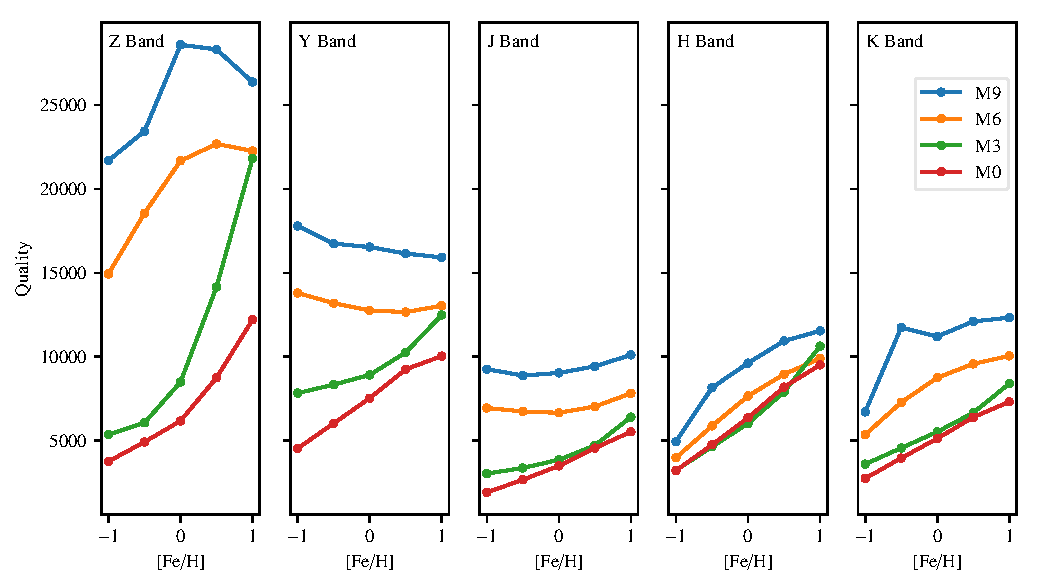
\includegraphics[width=0.99\linewidth]{figures/information-content/metalicity_effect.pdf}\\
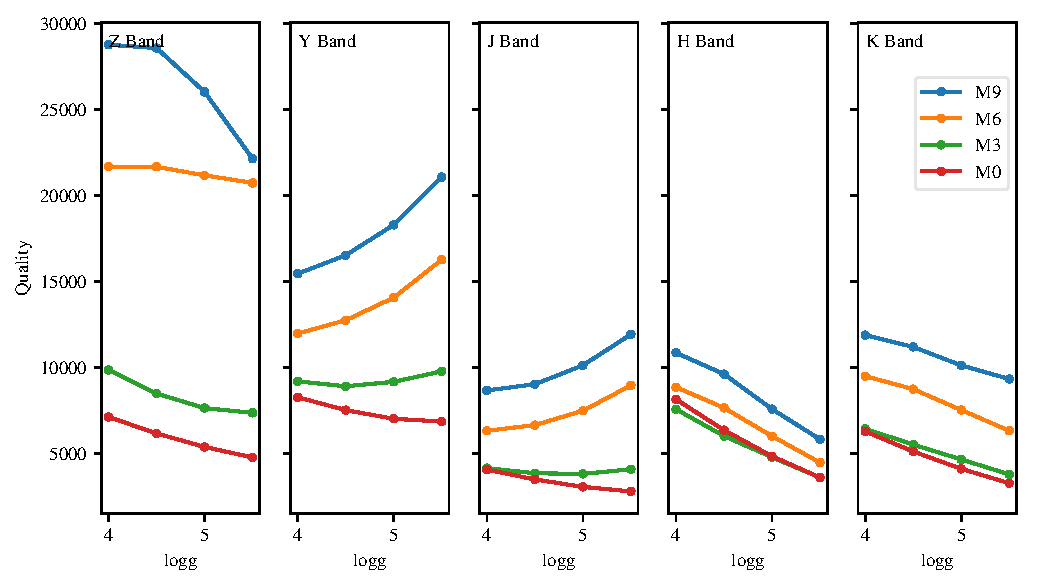
\includegraphics[width=0.99\linewidth]{figures/information-content/logg_effect.pdf}
\caption{Quality factor changes across spectral type and bands for variations in \feh{} and \logg{}. Broadening values are R=100\,000 and \(\vsini\) = 1.0\kmps{}. Top: Quality factor variation of \feh{} between -1.0 to 1.0 at a fixed \logg{}=4.5. Bottom: Quality factor variation of \logg{} between 4 and 5.5 with fixed \feh{}=0.0. Note a higher quality factor corresponds to an increased {RV} precision.}
\label{fig:deviations}
\end{figure}


\clearpage

\section{Updating {RV} precision software}
To undertake the calculation of RV precisions
A large section of this work involved optimizing the original code used in~\citet{figueira_radial_2016}.
Care needs to be taken to optimize the code. The original code used in~\citet{figueira_radial_2016} was slow, taking around 2 hours per simulation, this led to multiple weeks of processing time to compute the precision's for the original paper.

In this section we document the changes made to the code in the course of attempting to improving it. Features that change the derived {RV} precision are specifically documented in detail, with relative precision changes provided.

This work resulted in a submission of a publication\footnote{Available at \href{http://joss.theoj.org/papers/384bfc031df47ecef2d88328f63e5479}{http://joss.theoj.org/papers/384bfc031df47ecef2d88328f63e5479}} to \emph{The Journal of Open Source Software}\footnote{\href{http://joss.theoj.org/}{joss.theoj.org/}} (JOSS) {Neal and Figueria 2018 (in prep.)} with the source code openly available on \href{Github}{https://github.com/jason-neal/eniric}.


\subsection{Automated testing}
To insure that any changes made to the code did not change the underling results. This involved writing automatic tests for the software. This practice is crucial in computer science ins commercial software development but seldom done in research but is becoming more popular. \reference{works of software testing in research.}
Some work focused on testing ideology from computer science. Although not perfect implementation I began by adding automated tests to the code to check individual parts of it.
Before making changes I created automated tests that would confirm the functionality of pieces of the code. I could then make changes to the code, to improve the performance without worrying that the results were different.
Namely that the same precision were calculated in the end.

Functional test and unit tests.


 \subsection{Performance}
 \label{subsection:code_performance}
    There was a major performance bottleneck in the convolution stage, which increased the performance around 250\,X itself.
    The algorithm looped though the pixels in the spectrum, selecting out the necessary section around a given pixel with a comprehension list (for loop if inside range).
    Turning the result into a numpy array, performing the sum for that pixel and appending it to a list.
The performance issue was a python implementation detail to do with applying a comprehension list to a numpy array, then slicing the numpy array with the ends of the list, then converting it back into a numpy array, all of which is preformed on a very large spectrum array.
Creating a numpy boolean mask instead of the comprehension list, and applying the boolean mask to the array is much faster. Remaining entirely in the compiled numpy code and not converting between lists and numpy arrays (with involve type checking overhead).
This slow operation was done for every pixel/wavelength in the spectrum twice, once for each convolution.

caching convolution result to prevent recomputing the same values. \emph{Joblib}.  Also embarrassingly parallel so added multiprocessing support.

The convolution is still the slowest part. There are other methods that work on uniform spectra, which have not been tried to see how they affect the performance or {RV} precision results.
\textbf{Insert code samples.}


\subsection{Model extension}
The solution is to iterate over each pixel but create a mask array and use numpy indexing to select the required pixel span. (this remains in numpy)
These operations all remain in numpy so do not waste time converting between lists and numpy arrays, in which Python need to constantly check and convert the type of each item.

This shows a lesson in the usefulness of test driven development, or testing of code in science.


An normalization step was originally done after the convolution, to normalize out the effect of the convolution on a spectrum of 1s, due to the changing wavelength grids sampling. This was brought inside the main convolution by dividing the pixel by the convolution of a spectrum of ones at the same time. (again in numpy so it is quick)

Parallelization as embarrassingly parallel, the result of each pixel is independent of result of neighbours.

This is not a criticism of the work done by the original author (my supervisor). It is easier to modify a working system then to create one from scratch.

Computer code is not the important part in scientific exploration., although becoming more important in open source and reproducibility efforts. Often forgotten in

\# Handle any phoenix aces models.


\section{Numerical Gradient}
\label{sec:numerical_gradient}
One of the key insights from Equations~\ref{eq:optimal_weight} and~\ref{eq:dv_rms} is that the radial velocity error is inversely proportional gradient of the spectra, In numerically computing the {RV} precision, the result is dependent on the numerical method used to compute the gradient.
In original code used in~\citet{figueira_radial_2016} the gradient or slope is approximated using the forward finite difference method. The numpy package provides a function to calculate the gradient using a more advanced methods that compute a more precise gradient. In this section we explore the affect of improving the precision of the numerical gradient on the final {RV} precision.

The simplest way to calculate the derivative using finite difference methods~\citep{quarteroni_numerical_2000}. These arising from the Newton's definition of the derivative for a continuous function \(f(x)\) which should be familiar from introductory calculus:
\[f'(x) = \lim_{h \to 0} \frac{f(x+h)-f(x)}{h}~.\]

There are three common varieties of the finite difference,
 \[{FFD} = \frac{f(x+h)-f(x)}{h},  {CFD}=\frac{f(x+\frac{1}{2}h)-f(x-\frac{1}{2}h)}{h}, {BFD}=\frac{f(x)-f(x-h)}{h}\,,\] called the forwards ({FFD}), central ({CFD}), and backwards ({BFD}) finite differences respectively. The order of uncertainty on the {FFD}/{BFD} is \(\mathcal{O}(h)\) while for the {CFD} it is \(\mathcal{O}({h}^{2})\)~\citep{quarteroni_numerical_2000}. As the wavelength spacing between samples/pixels (h) is small the {CFD} will a more precise value for the gradient at each pixel.

In our case \(h\) is the difference in wavelength between the two pixels considered. In the {FFD} case the gradient at pixel \(i\) becomes:
\begin{equation}
\frac{\partial A_0(i)}{\partial\lambda(i)} = \frac{A_0(i+1) - A_0(i)}{\lambda(i+1)-\lambda(i)}, \hspace{2em} 1 \leq i \leq n-1.
\label{eq:ffd_precision}
\end{equation}
At each pixel the numerical derivative is evaluated to the average slope between itself and the following pixel and is an approximation to the derivative. This only extends to \(i= n-1\), where \(n\) is the number of points in the spectrum, and the last pixel is dropped from the {RV} calculation.\footnote{This is important in the case of Condition~\#2.}


The \emph{gradient}\footnote{Documentation available at \href{https://docs.scipy.org/doc/numpy/reference/generated/numpy.gradient.html\#id1 }{https://docs.scipy.org/doc/numpy/reference/generated/numpy.gradient.html\#id1}}  method provided in Numpy contains a more advanced numerical methods to calculate the derivative. It uses a \textit{compact difference} method~\citep{quarteroni_numerical_2000} which expand the finite differences using a Taylor expansion and then selecting coefficients to minimize the \textit{consistency error}.
From the Numpy documentation the consistency error here is \[\eta_i = \partial{f(x_i)}/\partial{x} -  [\alpha f(x_i) + \beta f(x_i +h_d) + \gamma f(x_i - h_s)],\] where \(h_s\) and \(h_d\) are the spacing to the left and right of \(i\) respectively.
With Taylor expansion this turns into solving a linear system of equations:
\[\begin{cases}
         \alpha + \beta + \gamma = 0\\
         -\beta {h_d} + \gamma {h_s} = 1\\
         \beta {h_{d}}^{2} + \gamma {h_{s}}^{2} = 0
    \end{cases}
\]
which result in the approximation of the gradient of the central values to be

\[\frac{\partial{f(x_i)}}{\partial{x}} = \frac{{h_{s}}^{2}f\left(x_{i} + {h_{d}}\right) + \left({h_{d}}^{2} - {h_{s}}^{2}\right)f\left(x_{i}\right) - {h_{d}}^{2}f\left(x_{i}-{h_{s}}\right)} {{h_{s}}{h_{d}}\left({h_{d}} + {h_{s}}\right)} + \mathcal{O}\left(\frac{h_{d}{h_{s}}^{2} + {h_{s}}{h_{d}}^{2}}{{h_{d}} + {h_{s}}}\right) \label{full_compact_difference}.\]

If the spectrum is evenly spaced ${h_{s}}={h_{d}}$  reduces to the standard second order {CFD} approximation:

\[\frac{\partial{f(x_i)}}{\partial{x}} = \frac{f\left(x_{i+1}\right) - f\left(x_{i-1}\right)}{2h} + \mathcal{O}\left({h}^{2}\right)\]


Applying this to our situation, similar to \eref{eq:ffd_precision}, we get:
\[\frac{\partial A_0(i)}{\partial\lambda(i)} = \frac{{\lambda(i-1)}^{2} A_0(i+1) + ({\lambda(i+1)}^{2}-{\lambda(i-1)}^{2}) A_0(i) - {\lambda(i+1)}^{2} A_0(i-1)} {\lambda(i-1)\lambda(i+1)(\lambda(i+1) + \lambda(i-1))}, \hspace{1em} 2 \leq i \leq n-1\]

with an uncertainty of \(\mathcal{O}\left(\frac{\lambda(i+1){\lambda(i-1)}^{2} + \lambda(i-1){\lambda(i+1)}^{2}}{\lambda(i+1) + \lambda(i-1)}\right)\).


{\red{} Wavelength spacing \(\delta\lambda\) between pixels is a function of \(\lambda\), Resolution and sampling choices. Can I do something with this??}

The \emph{gradient} function from Numpy implements central differences for the interior points, accurate to second order, and first order accurate one-sided (forward or backward) differences at the boundaries, computed using the same compact difference procedure.

\missingfigure{uncomment this one}
\begin{figure}
    \centering
   \includegraphics[width=0.8\linewidth]{figures/information-content/spectral_gradients}\\
    \caption{Visualization of the numerical gradient of some spectral lines. Top: The two spectral regions of a stellar spectrum the left hand slide contains short lines near the normalized continuum while on the right a single deep absorption line is shown. Bottom: The numerical gradients for the spectra shown in the top panels; the original {FFD} method is displayed  with \emph{blue squares} while numpy gradient is shown with \emph{green stars}. The \emph{orange circles} are the {FFD} version shifted to the mid-points between pixels for illustrative purposes.}
    \label{fig:gradients}
\end{figure}


%!TEX root = ../thesis.tex

\begin{table}
    \caption{The affect of the numerical gradient function on RV precision. The band label \(\rm VIS\) indicates the visible band while  \(\rm CARM_{VIS}\)  and \(\rm CARM_{NIR}\)  indicate the two wavelength bands of the CARMENES spectrograph. \(\Delta\lambda\) is a wavelength shift applied to analyse the pixel weights at the middle of their FFD gradients for comparison only.}
    \begin{tabular}{ccccccc}
        \toprule
%% Band & $\lambda$ range\_min & wl\_max &  dy/dx   & gradient & Q(dy/dx) & Q(grad) & Q(frac) & RV(dy/dx) & RV\_adj &    RV(grad)    &    RV(frac\_grad)    & RV(frac\_adj)          \\
  &   $\lambda$ range & \multicolumn{3}{c}{RV\(_{rms}\) (\mps{})} & \(\Delta\) RV ratio& \(\Delta\) RV ratio\\
 Gradient method&  &  A &   B & C & (B-A)/A & (C-A)/A \\
 Band  &  \si{\micro\meter} & FFD & FFD+\(\Delta\lambda\) &  CFD &  \% & \% \\
    \midrule
VIS & 0.38 -- 0.78 & 16.1 & 16.2 & 16.9  & 0.6 & 4.9\\
\(\rm CARM_{VIS}\) & 0.52 --  0.96 & 20.9 & 21.0 & 22.0 & 0.3& 5.2 \\
Z & 0.83 -- 0.93 & 76.9 & 77.0 & 78.8  & 0.1 & 2.5\\
Y & 1.00 -- 1.10 & 78.3 & 78.5 & 83.8 & 0.2 & 7.0 \\
J & 1.17 -- 1.33 & 149.3 & 149.4 & 156.4 & 0.1 & 4.7 \\
H & 1.50 -- 1.75 & 119.4 & 119.5 & 122.3 & 0.1 & 2.5 \\
K & 2.07 -- 2.35 & 153.4 & 153.7 & 157.7  & 0.2 & 2.8\\
\(\rm CARM_{NIR}\) & 0.96 -- 1.71 & 46.1 & 46.2 & 48.0 & 0.1& 4.2 \\
NIR & 0.83 -- 2.35 & 36.9 & 36.9 & 38.2 & 0.1 & 3.6  \\
    \bottomrule
    \end{tabular}\label{tab:numerical_gradients}
\end{table}


In \fref{fig:gradients} we visualize the gradients of two small spectral regions computed with the original {FFD}, and the higher precision version incorporated in numpy's gradient function.
The top panels contain the spectrum in the small regions shown, indicating a large spectral line and three small lines near the continuum respectively.
The derivative of the spectra is shown in the bottom panel with the {FFD} method shown with \emph{blue squares} and the numpy gradient shown in \emph{green stars}.
The \emph{orange circles} are the same as {FFD} but shifted horizontally to the midpoints between  pixels.
This is for illustrative purposes and to assess the effect of this offset when calculating the pixel weights.

There a three notable features observed between gradient methods.
The first, which is expected from the {FFD} formulation is that the {FFD} gradient is offset to the left.
The second is that when the horizontal offset is adjusted (orange circles) the gradients lie along the same curve.
Both methods are trying to approximate the real gradient function of the spectrum and is again expected.
The most important feature observed in this though is that there is a slight over-estimate of the gradient by the {FFD} method at the peaks.
In the bottom panels of \fref{fig:gradients}, the points of highest gradient are always from the {FFD} method (blue/orange).
This is the case for all spectral lines and as the optimal pixel weights are proportional to the gradient squared the {FFD} method will apply slightly higher pixel weights to these values, two points per line in the spectrum.
The {FFD} will therefore produce a slightly smaller \(\delta V_{\rms}\) error compared to the more precise gradient function.

In \tref{tab:numerical_gradients} we calculate the  \(\delta V_{\rms}\) using both gradient methods to determine their relative effect on the {RV} precision.

We took a {PHOENIX-ACES} spectrum with \txteff{}=3\,900\K{}, corresponding to {{M0}} spectral type.
The full theoretical precision is calculated (no telluric masking applied) with no rotational or instrumental broadening and the maximum of the continuum of each band scaled to 1.
In this case the {RV} precisions are not comparable between bands and are only to assess the direct effect of the changing the numerical gradient.
The bands name and the spanned wavelength are given.
The columns A, B, C are the {RV} precision for the different gradient methods.
The \(\delta V\) ratios are the relative difference in {RV} when changing from method A (the original {FFD}) to methods B and C.
In this table column B is the {FFD} method but with the wavelength shifted to in between pixels, corresponding to the orange circles in \fref{fig:gradients} while column C is the more precise gradient from numpy.

We find that changing to use the gradient from numpy increases the \(\delta V_{\rms}\) by 2.5--7\%, (decreasing the {RV} precision), due to the over-estimated gradient from the {FFD} method.
As the pixel weights \eref{eq:optimal_weight} are also proportional to \({\lambda}^{2}\) column B was computed to assess the effect of the slight wavelength offset on the {RV} precision, visible in \fref{fig:gradients}.
This small wavelength shift red-ward does changed the {RV} precision by 0.1--0.6\% which is an order of magnitude smaller than the relative change when using numpy's gradient method.

Changing the method of numerical derivatives will change all the precision values given in the~\citet{figueira_radial_2016}. This is a small impact on on the precision compared to other components of the {RV} precision. For instance from \eref{eq:rv_SNR} a increase in \(\delta V_{\rms}\) of between 2.5--7\%  could equally be caused by a small decrease in the \snr{} from 100 (the value used in~\citet{figueira_radial_2016}) to between 95--98.

The current version of the software is now implemented with the gradient method provided by numpy package.

\subsection{Masking Function}
\label{subsec:masking_function}
Another change made to the software is in the application of the masking function, and the treatment of telluric lines. As suggested in~\cite{connes_absolute_1985} and~\cite{bouchy_fundamental_2001} a custom masking function can be applied to the individual pixel weights in \eref{eq:optimal_weight}, such as:

\[W'(i) = W(i)M(i),\label{eq:mask_function}\] where \(M(i)\) is the masking function and \(W'(i)\) are the modified pixel weights.
This masking function can be used in particular for the removal of telluric lines, setting those weights to zero and is in essence what is done when wavelength selection is preformed; assigning zero weight to all pixels outside the desired wavelength range.

This masking function can be used to easily apply the three conditions presented in~\citet{figueira_radial_2016}. First  the 3 masking functions will be defined, then followed by the quantification of how they differ from the previous implementation. The subscripts on the masking functions correspond to the three conditions.
\begin{align}
M_1(i) &= 1 \label{eq:mask1}\\
M_2(i) &= \begin{cases}
0, \hspace{1em} T(i) < \tau\\
1, \hspace{1em} T(i) \ge \tau\\
\end{cases}\label{eq:mask2}\\
M_3(i) &= {T(i)}^{2} \label{eq:mask3}
\end{align}

Here, \(T(i)\) is the telluric transmission spectrum, while \(\tau\) is the transmission depth cut-off. For instance to mask out telluric lines deeper than 2\%,  \(\tau\) would be set at 0.98.

\begin{itemize}
    \item Condition~\#1:
    The first mask, \(M_1\), is the simplest case in which all pixel weights are treated equally. No telluric line masking is considered.

    \item Condition~\#2:
    In the second mask, \(M_2\), the telluric line transmission, \(T(i)\) is used to create a boolean mask of 0's and 1's. When applying this mask to the pixel weights, the pixels effected by telluric lines have 0 weight, removing their contribution to the {\red{} \(RV_{\rms}\)}. Accounting for seasonal variation in Earth's barycentric motion can be easily incorporated into this mask, widening the regions masked out.

    \item Condition~\#3:
    The third mask, \(M_3\), assumes the application of perfect telluric correction consistent with Condition~\#3. The pixel weights are modified by dividing the flux variance by the square of the transmission spectrum \reference{cite the equation when I refer to it}. As the flux variance is the denominator of \eref{eq:optimal_weight}, this is equivalent to multiplication of the weights by a mask of the form \(M_3\).
\end{itemize}

Having the three masks defined in this way makes the implementation of the {RV} precision simpler. In the original version there were three separate implementations, one for each condition. With this, \todo{Check this if it is previous}{as mentioned previously} there was a issue with the implementation of Condition~\#2.

\subsubsection{Masking order}
\label{subsubsec:masking_order}
The order in which the masking is preformed is also important. Masking should be applied only after calculation of the pixel weights. As the pixel weights depend on neighbouring points (through the calculation of the gradients), prematurely removing pixels will affect the precision results.

The original implementation of Condition~\#2 did just this, splitting the spectra into small sections in between the masked off telluric lines. The {\red{}\(RV_{\rms}\)} is calculated for each section and then the results are combined as the weighted error in {\red{} \eref{XXX}} \todo{weighted sum equation}. Analytically this identical to masking the pixel weights with \(M_2\) but not in practice when numerically implemented. \todo{Should I show the working of analytical working out of this in an appendix, or here?}

When the spectrum is split into small sections the number of edges increases and the number of pixels affected by any edge effects increases. Using the {FFD} method to compute the gradient the last pixel is removed/lost. A spectrum split in \(m\) sub-spectra will therefore lose \(m\) pixels due to edge effects (instead of only 1 pixel with the full spectrum).
Even the numpy gradient is not immune to the edge effects in the sub-spectra when splitting the spectrum first. Even though there is no pixels lost, the first and last pixels of each sub-spectra are computed using forward or backward differences, rather than central differences (as they would be in the full spectrum). Hence the gradients and weights of some pixels are slightly changed due to the splitting occurring first.

We quantify the effect of splitting the spectrum before and after calculating the weights in \tref{tab:mask_ordering}. The columns label \emph{Split} represents splitting the spectrum before calculating the pixel weights while the \emph{Mask} columns calculate all the pixel weights first and then apply the \(M_2\) mask. The difference in {RV} precision between both situations and for both gradient methods are given.
For the {FFD} gradient the ordering of masking changes decreases the {\red{}\(RV_{\rms}\)} by 0.2--0.7\%, while for the numpy gradient it is increase but an order of magnitude smaller between 0.01--0.13\%.
The {FFD} gradient is causes a larger difference as points that were masked out are now included where as with the numpy gradient the end values are always included but their gradients are slightly changed.
The last column is the difference ratio between the \emph{Mask} column of both gradient method, this is consistent with \tref{tab:numerical_gradients} with the differences from two gradient methods between 2--7\%.
It shows that the difference from changing order of masking is 1-2 orders of magnitude smaller than changing the gradient method.

The code has been adjusted to consistently apply the masking after the pixel weights are calculated. This retains the most pixels, with the more accurate pixel weights. It has also been changed to just apply \(M_2\) rather than splitting and performing the weighted error calculation.\todo{did I check this was equivalent} This simplifies the implementation in calculating the {RV} precision.

%!TEX root = ../thesis.tex

\begin{table}
    \centering
    \caption{Relative {RV} precision difference for Condition \#2 due to spectral splitting and order of applying the pixel mask. The ratio are the difference between Split and Masked implementations with the same gradient calculation. The last column is the ratio between the Masked versions using the FFD and numpy gradient methods and are consistent with \tref{tab:numerical_gradients}. Results a for an M0 spectral type, with vsini=1.0 and R=100,000.}
    \begin{tabular}{c|ccc|ccc|c}
        \toprule
        & Split & Masked & \(\Delta\)Ratio & Split & Masked & \(\Delta\)Ratio & Masked \\
        Gradient & \multicolumn{3}{c|}{FFD} & \multicolumn{3}{c|}{Numpy} & \(\Delta\)Ratio\\
        Band & \mps{} & \mps{} &  \%  & \mps{} & \mps{} &   \% & \% \\
        \midrule
        Z &  7.42 &  7.38 & -0.66 &  7.76 &  7.77 & 0.13 & 5.3\\
        Y &  4.75 &  4.74 & -0.22 &  5.06 &  5.06 & 0.06 & 6.8\\
        J & 18.58 & 18.53 & -0.29 & 19.57 & 19.57 & 0.01 & 5.6\\
        H &  6.08 &  6.05 & -0.53 &  6.25 &  6.26 & 0.08 & 3.5\\
        K & 32.21 & 32.14 & -0.22 & 33.48 & 33.49 & 0.05 & 4.2\\
        \bottomrule
    \end{tabular}\label{tab:mask_ordering}
\end{table}

{\rd{} The results from these spectra for conditions \#1 and \#3 are consistent with Figueira et al. 2016. \todo{put this some where}}


{\red{} For Condition~\#2 in which there was an error there is no meaningful relation between the new and old values. \todo{put this line elsewhere.}}


\subsection{Atmospheric masking bug}
\label{subsec:condition_two_bug}
One thing that was revealed in testing was that there was an error in the application of Condition~\#2. When the telluric mask was shifted to account for barycentric motion of the earth, and the condition of 3 consecutive pixels in the telluric spectra being lower than the limit (due to the higher sampling) there was an software bug,


A check for this issue was discovered using this unit test.
\begin{lstlisting}[language=Python, caption=Example unit test to catch masking bug.]
def test_telluric_masking(wavelength, transmission):
    mask = telluric_mask(transmission, depth=0.98)
    mask = barycenter_shift(mask)

    # Checks that the mask is still masking out all telluric lines.
    assert np.all(transmission[mask] > 0.98)
\end{lstlisting}
The assert statements checks that when the mask is applied to the transmission spectrum again all of the values are outside of any deep telluric regions. A test like this would have caught this bug.

This bug means that all the {RV} precision values for Condition~\#2 published in~\citet{figueira_radial_2016} incorrect. As the applied masking was unevenly applied~\citet{figueira_radial_2016} the new values {RV} precision values do not all change in the same proportion or direction. Some specific wavelengths and resolutions are essentially unchanged while other results change by over 20\mps{}.  Even though there is an error with condition~\#2 they do not change the overall conclusions of the paper. These are \todo{add conclusions not affected}

\subsection{SNR scaling}
\label{subsec:snr_scaling}
To analyse the relative precision of different spectra they need to normalized to a common reference point. In this section we detail how this was originally done and how this was changed to be adaptable to any library spectra and any reference band.

In the original code this was selected to be a \snr{} per pixel of 100 at the centre of the \textit{J}-band at 1.25\si{\micro\meter}. The normalization values for each band, \(\vsini\) and resolution combination were hard-coded into the analysis. This made it impossible to easily adapt the code to other spectra or parameter combinations.

An automated \snr{} scaling procedure was created to remove the hard-coded values. This updated code finds the centre point of the band of reference for the given spectrum. Totals the photon count across one resolution element, \(\delta\lambda\), and then takes the square root. This is using the definition of the \snr{} as \({SNR} = \sqrt{N}\) for large N. This value is then used to scale the spectrum such that the \snr{} at the reference point is the desired value.

\begin{equation}
    SF =  \frac{\sqrt{\sum{\delta\lambda} A}} {SNR_{desired}}
\end{equation}

\textit{SF} where \textit{SF} is the scaling factor, \(\sum_{\delta\lambda} A\) is the sum of the point in one resolution element and \({SNR}_{desired}\) is the desired \snr{} level requested.

This automated procedure enabled {\red{}\textbf{4}} different features.
\begin{itemize}
\item The ability to analysis other spectral models, not just corresponding to {M0}, {M3}, {M6}, {M9} spectral types.
    - Scaling to a \snr{} per pixel level other than 100.
\item    A \snr{} per pixel other than 100 can be selected.
    - Allowing for other sampling levels (if desired)
\item      Not restricted to a model with 3 samples per resolution element.
\item Different reference bands available.
    Results are not limited to being referenced from the \textit{J}-band. For instance the {RV} precision can now be calculated for a given \snr{} at the centre of the \textit{K}-band. This was one the features requested for the Exposure Time Calculators precision values. For {NIRPS} we provided precision values relative to each individual band, while for {SPIRou} they were relative to the {J}- and {H}-bands.
\end{itemize}
The default values for the \snr{} scaling a still 100 at the centre of the \textit{J}-band, but there is now options to easily change these values.

The centre of each band was visually checked to ensure that there were no spectral lines at the reference locations> If a line was present at the reference point its depth variability across spectral types would affect the \snr{} scaling levels at a greater than the normal change in continuum amplitude/shape.\todo{is this needed}

As shown in \eref{eq:snrequation} the {RV} precision is inversely proportional to the \snr{} level. To access the {RV} precision of any of the values in Table at a different \snr{} level you can apply the following

\begin{equation}
\rm RV_{SNR2} = RV_{SNR1} * \frac{SNR1}{SNR2}
\end{equation}

\todo{SNR plot/diagram}
\section{{SPIRou} and {NIRPS} {ETC}}\label{sec:spirou_nirps_etc}
Having this tool to calculate {RV} precisions efficiently lead to contributions to the Exposure Time Calculators (ETC) for both the {SPIRou} and {NIRPS} spectrographs.

In September 2017 we were requested to provide precision calculations for the {SPIRou} ETC\footnote{\url{http://www.cfht.hawaii.edu/Instruments/SPIRou/SPIRou_etc.php}}. These were the same table as~\citet{figueira_radial_2016} but with a each band referenced to 100~{SNR} in its own band. The modification to use the centre of any band was made to fulfil this request. Notes on the telluric correction issue affect on Condition~2.

In May 2018 we were requested to provide precision calculations for the {NIRPS} {ETC}.\@ This extended the spectral range from {M0}, {M3}, {M6}, {M9} at 3\,900, 3\,500, 2\,800, 2\,600\K{} respectively, but to all temperatures between 2\,500 and 4\,000\K{} inclusively. This provides a finer resolution coverage over the M spectral type, allowed by the {PHOENIX-ACES} library.
Instrumental resolutions of 75,000 and 100\,000 were requested to match the {NIRPS} instrument.
The \logg{} and metallicity, sampling rate remained at the~\citet{figueira_radial_2016} levels of 4.5, 0.0 and 3 respectively.
Precisions were provided for \snr{} of 100 relative to the \emph{J}-, \emph{H}-bands as well as to each band individually. Artigua 2018. (private communication 2018)\todo{Check how to cite priv communication properly} suggested the truly relevant value is the \snr{} in \emph{H}-band for {NIRPS} radial velocities.

The results can be manually generated using ``eniric'' with the following incantation (after installation and configuration of phoenix library spectra.)
\textbf{A table of the precisions created for the {NIRPS} ETC are provided as an online table to our publication} \textit{Neal et al. 2018b (in prep.)}\footnote{Available at \href{blah}{blah}} \unfinished{Inlcude correct links}


These values were both calculated and provided using the {FFD} gradient and with the incorrect masking order for Condition~\#2, splitting before calculating the pixel weights. As we demonstrated in \sref{sec:numerical_gradient} and~\ref{subsubsec:masking_order} these have a {RV} precision \(\sim\)2--7\% better than what would be computed with the current implementation.


\section{ Updated Figueira 2016 results}
\todo{comparison of plots} figueira eta la plot 1, eniric plot

\begin{figure}
    \centering
    \begin{tabular}{cc}

    \includegraphics[width=0.48\linewidth]{figures/information-content/Rvprec_vsini1.pdf} &  % Figueria plot
    \includegraphics[width=0.47\linewidth]{figures/information-content/precision_fourpanel.png}\\ % eniric plot
    \end{tabular}
    \caption{Left: Figure 1 from \citet{figueira_radial_2016}, Right: The same style figure with values updated from this work, computed with \emph{eniric}. The main difference is the area of shaded region due to the problem with Condition~\#2 (which is the upper edge).}
    \label{fig:my_label}
\end{figure}
\todo{Change to 55 m/s upper limit?}

\section{ metalicity / logg extension}



\section{Application to CARMENES spectra}

- target selection

- preparation of observed spectra

- Barnards star (artigau 2018 comparision)


This work is work in progress. So far only 1 of 8 planned CARMENS spectra have been telluric corrected to calculate the RV precision.

{I can calculate the rv precision from models though.}

	%!TEX root = ../thesis.tex
%5-Discussion

\chapter{Discussion}  % Main chapter title

\label{cha:Chapter5} 

%----------------------------------------------------------------------------------------
%	SECTION 1
%----------------------------------------------------------------------------------------

\section{Main Section 1}



%-----------------------------------
%	SUBSECTION 1
%-----------------------------------
\subsection{Subsection 1}


%-----------------------------------
%	SUBSECTION 2
%-----------------------------------

\subsection{Subsection 2}

%----------------------------------------------------------------------------------------
%	SECTION 2
%----------------------------------------------------------------------------------------

\section{Main Section 2}



	%!TEX root = ../thesis.tex
%6-Conclusions

\chapter{Conclusions}  % Main chapter title

\label{cha:conclusions}

%--------------------------------------------------------------------------------------------------------------------------------------------

\section{Conclusions from Paper}
\label{sec:conclusions}

This work explored two methods to try and detect the faint spectra of stellar companions, using high resolution near-infrared spectra.
Two different methods were explored with many limitations uncovered.

The objective of the observations acquired in this program was to a apply the differential technique.
For the differential technique the observations need to be sufficiently separated, such that the {RV} of the companion is greater than the {\fwhm} to avoid spectral cancellation of the companion.
Unfortunately, due to operational reasons, this condition was not met.
As such we employed an alternative method, that we termed the spectral recovery, which ended up revealing different difficulties.

For the spectral recovery the host-companion {RV} separation should also ideally be greater then the {\fwhm} to avoid blended lines.
The spectral mismatch between models and reality in the \nir{}negatively affects the performance of the synthetic recovery technique on the observed spectra.
With all these effects we are unsuccessful in the detection of the \nir{}spectra of {BD} companions, with the mass upper-limits set at 600~\Mjup{} from the synthetic recovery technique.

This work highlights many of the difficulties when dealing with the spectral recovery of \nir{}spectra.
The obstacles to overcome are the data reduction of \nir{}CMOS detectors, that are not yet at the level of visible CCDs, along with a precise telluric correction and wavelength calibration (two interrelated aspects, as thoroughly discussed).
Another important aspect is the mismatch between \nir{}high-resolution spectra and the observed spectra.
In spite of the continuous effort of the modelling community, our work, along with several cited contemporary ones, shows that this mismatch is still one of the main factors preventing us from performing spectral recovery in the \nir{}.\@ This work highlights that this is a compound problem for Brown Dwarfs, for which the spectral models are worse informed due to lack of observations at high-resolution.

Other than the improvement of the spectral models, the observing community can increase their odds of success by paying attention to the scheduling of observations and the wavelength domains to explore.
Our work shows that observing in the areas of lower telluric absorption, as is frequently done, is not a guarantee of success due to the scarcity of deep lines in cold objects.
Moreover, due to the mismatch between models and observations, the ability to obtain a first spectra before settling on a wavelength range, or changing settings on the fly, is extremely useful for the success of these campaigns.

We hope that this work can act as a guide for the planning of future observations of targets with faint {BD} and planetary companions with the upcoming generation of high resolution spectrographs in the near- and mid-infrared such as {CRIRES+} and JWST observations.


\todo{NIR analysis work}{Finish off this}



\section{Future Work}

Future of {RV} precision

Machine learning techniques to the RV precision measured on the spectral library.
For instance can it fit models of stellar parameters, or instrument/rotational broadening.
Similar to theory?


A way to combine the information for the \logg{} and \feh{} observed in section 6.X.X...


Machine Learning RV precision of {PHOENIX-ACES} models.







\subsection{Future implementation}
\todo{reduce this for the conclusions}
\label{subsec:future}
\subsubsection{High resolution instrumentation}
\label{subsubsec:highres}
The future of high resolution near- and mid- IR spectrographs is looking bright, with many new ground- and space-based instruments currently being developed.
Notable examples include CARMENES (550--1710\nm{},  R=82\,000) which is now operational~\citep{quirrenbach_carmenes_2014}, while SPIRou (980--2350\nm{},  R=73\,500)~\cite{artigau_spirou_2014} and NIRPS (970--1810\nm{}, R=100\,000)~\cite{bouchy_nearinfrared_2017} are still being assembled and installed.
The eagerly awaited {JWST} \textbf{cite} will also be launched soon\footnote{Recently pushed to around May 2020} providing observations in both the \nir{} (600--5300\nm{}, R=2700) and mid-IR (4900--28\,800\nm{}, R$\sim$1550--3250) regions without contamination from \textrm{our} atmosphere.

The upgrade of CRIRES to CRIRES+~\citep{dorn_crires_2016} will increase the wavelength coverage of a single shot capture by at least a factor of 3--5.
This larger wavelength span would be extremely beneficial for the \textchisquared{} performance of the spectral recovery method, increasing the number of useful lines and spectral features to be fitted with the models.

On the modelling side, there are continual improvements in atmospheric modelling and their associated synthetic spectral libraries: as seen with the evolution of the {BT-Settl} models~\cite{allard_btsettl_2013}.
With additional physics and improved line lists and solar abundances~\citep [e.g.][]{asplund_chemical_2009,caffau_solar_2011}, the synthetic libraries are reaching a better agreement with \nir{} observations.
An improved agreement between the \nir{} observations and synthetic spectra will be crucial to improve the performance of the spectral recovery technique presented here.

Although not successful with the CRIRES data used here, the instrumental stage is set to attempt these techniques presented here using the next-generation of high resolution spectrographs.
The lessons learned in this analysis need to be taken into account in order to achieve the best chance of a successful detection.


\section{Conclusions from paper}
\label{sec:conclusionsfrom paper}
This work aimed at pushing down the detection limit of faint companions, using high resolution near-infrared spectra.
Two different methods were explored with many limitations uncovered.

The objective of the observations acquired in this program was to a apply the differential technique.
For the differential technique the observations need to be sufficiently separated, such that the {RV} of the companion is greater than the {FWHM} to avoid spectral cancellation of the companion.
Unfortunately, due to operational reasons, this condition was not met.
As such \textrm{we} employed an alternative method, that \textrm{we} termed the spectral recovery; this method is in principle fully equivalent, but ended up revealing different difficulties.

For the spectral recovery the host-companion {RV} separation should also ideally be greater then the {FWHM} to avoid blended lines.
The spectral mismatch between models and reality in the \nir{} negatively affects the performance of the synthetic recovery technique on the observed spectra.
With all these effects \textrm{we} are unsuccessful in the detection of the \nir{} spectra of {BD} companions,  with the mass upper-limits set at 600\Mjup{} from the synthetic recovery technique.

This work highlights many of the difficulties when dealing with the spectral recovery of \nir{} spectra.
The obstacles to overcome are the data reduction of \nir{} CMOS detectors, that are not yet at the level of visible CCDs, along with a precise telluric correction and wavelength calibration (two interrelated aspects, as thoroughly discussed).
Another important aspect is the mismatch between \nir{} high-resolution spectra and the observed spectra.
In spite of the continuous effort of the modelling community, \textrm{our} work, along with several cited contemporary ones, shows that this mismatch is still one of the main factors preventing us from perform spectral recovery in the \nir{}.
This work highlights that this is a compound problem for Brown Dwarfs, for which the spectral models are worse informed due to lack of observations at high-resolution.

Other than the improvement of the spectral models, the observing community can increase their odds of success by paying attention to the scheduling of observations and the wavelength domains to explore.
Our work shows that observing in the areas of lower telluric absorption, as is frequently done, is not a guarantee of success due to the scarcity of deep lines in cold objects.
Moreover, due to the mismatch between models and observations, the ability to obtain a first spectra before settling on a wavelength range, or changing settings on the fly, is extremely useful for the success of these campaigns.

We hope that this work can act as a guide for the planning of future observations of targets with faint {BD} and planetary companions with the upcoming generation of high resolution spectrographs in the near- and mid- infrared such as CRIRES+ and {JWST} observations.





	\appendix
	\unfinished{Precision table needs fixed up}	
    %%!TEX root = ../thesis.tex
% Appendix Template

\chapter{NIR Precision amendment} % Main appendix title

\label{AppendixX} % Change X to a consecutive letter; for referencing this appendix elsewhere, use \ref{AppendixX}

During the improvement of the NIR precision software a significant error was discovered in the telluric masking. Basically the algorithm to detect the edges of telluric lines did not work correctly. This meant the telluric masks applied in the second criteria of \citet{figueira_radial_2016} are significantly incorrect.

Here we include the table from Figueira 2016 with the condition 2 being significantly different. 
The are some slight modifications of the conditions 1 and 3, or the order 0.1 .from original values. 


\unfinished{needs the rounding performed.}{table}

% Load in the ENIRC precision data

%\DTLsetseparator{ }
%%\DTLloaddb{precision}{./appendices/precisiondata2017.tsv}
%
%\begin{longtable}{cccc}
%    \caption{Results of the simulations described in Sect.\,........}\label{TableData}
%    \\
%    \hline\hline
%    Simulation & $\sigma_{RV}$(Cond.\,1) & $\sigma_{RV}$(Cond.\,2) & $\sigma_{RV}$(Cond.\,3) \\ 
%    (SpTp - Band - $v.sin{i}$ - R) & [m/s]& [m/s] & [m/s]%\\
%    \hline
%    \endfirsthead
%    \caption{continued.}%\\
%    \hline\hline
%    Simulation & $\sigma_{RV}$(Cond.\,1) & $\sigma_{RV}$(Cond.\,2) & $\sigma_{RV}$(Cond.\,3) %\\ 
%    \hline
%    \endhead
%    \hline
%    \endfoot
%    \caption{NIR precision}
%    \centering
%
%    \toprule
%    &&&&\\
%    %\DTLforeachkeyinrow{precision}{\id=id, \condone=prec1, \condtwo=prec2, \condthree=prec3}{
%     %    \\
%     %    \id & \condone & \condtwo & \condthree 
%     %    }
% 
%\end{longtable}


\DTLsetseparator{ }
% \DTLloadrawdb{precisions}{precision_results_2017_ref_band-J_snr-100.0.dat}%

\longtab[2]{
    \begin{longtable}{cccc}
        
        \caption{Correction to results of the simulations described in Table\,A.1 of \citet{figueira_radial_2016}.}\label{TableData}
        \\
        \hline\hline
        Simulation & $\sigma_{RV}$(Cond.\,1) & $\sigma_{RV}$(Cond.\,2) & $\sigma_{RV}$(Cond.\,3) \\ 
        (SpTp - Band - $v.sin{i}$ - R) & [m/s]& [m/s] & [m/s]\\
        \hline
        \endfirsthead
        \caption{continued.}\\
        \hline\hline
        Simulation & $\sigma_{RV}$(Cond.\,1) & $\sigma_{RV}$(Cond.\,2) & $\sigma_{RV}$(Cond.\,3) \\
        \hline
        \endhead 
        \hline
        \endfoot
        ...&....&...&precision\_results\_2017\_ref\_band-J\_snr-100.0.dat\\
        %\DTLforeach*{precisions}{\sim=id, \condone=prec1, \condtwo=prec2, \condthree=prec3}{%  \DTLiffirstrow{}{\\}  if first row don't add a new line at start.
        %\DTLiffirstrow{}{\\}\sim & \condone & \condtwo & \condthree
        %}
        
    \end{longtable}
}
	%!TEX root = ../thesis.tex
% Appendix Template

\chapter{Artifacts in Optimal Extraction} % Main appendix title

\label{appendix:artifacts}


% Table of nods optimally reduced replaced by rectangular extraction and bad pixel replacement.
%!TEX root = ../thesis.tex
% Table of nods replaced for correction. 
\change{Maybe transpose \tref{tab:nod_replacement} to be shorter?}{}
\change{CHANGE \# into the ESO identification number 1b 2a etc}
\begin{table}
    \caption{Identification of all the optimally reduced nod spectra which had artefacts that were replaced by the rectangular extractions, corrected for bad pixels. The numbers represent the position in the nod cycle ABBAABBA. The number of the observation for each target is given by \#.}
    \label{tab:nod_replacement}
    \centering
    \begin{tabular}{cccccccc}
        \toprule
      & & \multicolumn{4}{c}{Detector}& \\
         Target  & \#  & 1 & 2 & 3 & 4 & Total \\ 
        \midrule
        \object{HD 4747}   & 1 & 8 & 5, 8 & 8 & 1, 5, 8 & 7\\
        \object{HD 162020} & 1 & - & 7, 8& - & - & 2\\ 
        \object{HD 162020} & 2 & - & 2 & - & 8 & 2\\ 
        \object{HD 167665} & 1 & 2, 4 & 8 & 1, 6 &  4, 5 & 7\\ 
        \object{HD 167665} & 2 & 2 & 3 & 1 & 8 & 4\\ 
        \object{HD 167665} & 3 & 6 & 3, 7 & - & 8 & 4\\ 
        \object{HD 168443} & 1& - & - & - & 7, 8 & 2\\ 
        \object{HD 168443} & 2 & - & 2, 4 & 6 & 8 & 4\\ 
        \object{HD 202206} & 1 & - & 6, 7& 1& - & 3\\ 
        \object{HD 202206} & 2 & 5 & - & 7,8 & - & 3\\ 
        \object{HD 202206} & 3 & 8 & 3 &  6 & 6 & 4\\ 
        \object{HD 211847} & 1 & - & 5, 7 & 2 & 4 & 4\\ 
        \object{HD 211847} & 2 & 2 & 1, 7 & 7 & 8 & 5\\ 
        \object{HD 30501}  & 1 & 7 & 7 & - & 8 & 3\\ 
        \object{HD 30501}  & 2 & 7, 8 & 3, 5, 7, 8 & 2, 7 & 2, 3&10 \\ 
        \object{HD 30501}  & 3 & 4, 8 & 2, 6, 7& 4, 8 & 7& 8\\ 
        \object{HD 30501}  & 4 & 1, 2, 4 & 3 & 5, 6 & 6 & 7\\
         \midrule
            &&&&&& 79/544\\
    \bottomrule
    \end{tabular} 
\end{table}

As mentioned in \sref{subsubsec:reductionartifacts} there were artifacts observed from the optimal reduction of the DRACS pipeline. In \tref{tab:nod_replacement} we provide a list of all the specific nods for each observation and detector that we observed artifacts and replaced with our explained method.  

With 8 nods per observation, and 4 detectors for the 17 observation there are 544 individual nod spectra. \tref{tab:nod_replacement} identifies 79 individual nods that contain artifacts which is 14.5\%.   Only 16/68 (23.5\%) detector observations have nods without any artifacts and no single observation has no artifacts in any nod spectra across the 4 detectors.




In this appendix we also provide more example images of the artifacts observed from the optimal reduction of the DRACS pipeline. We have selected one observation and detector for each observed target to show a variety of the artifacts observed.

In each image the top panel contains the 8 nod spectra extracted using the optimal method, including variance weighting. The middle panel contains the rectangular extraction (sum of the aperture), including the bad pixels.

It is clear that the large extracted artifacts occur due to single spikes observed in the rectangular extraction. What is unclear is why it only occurs some of the time.
 

\todo{THESE need to be properly selected and a caption given, one without any artifacts also?}
\todo{Style needs to be tweaked also}
 
 \begin{figure}
     \centering
     \includegraphics[width=0.7\linewidth]{figures/reduction/bp_plots/extraction_comparision_HD4747-1_chip_1}
     \caption{Artifact example for HD4747. Optimal and rectangular nods, continuum normalized and vertically offset.}
     \label{fig:artifact_example1}
 \end{figure}
 \begin{figure}
     \centering
     \includegraphics[width=0.7\linewidth]{figures/reduction/bp_plots/extraction_comparision_HD4747-1_chip_2}
     \caption{Same as \fref{fig:artifact_example1} but for HD162020. {\red change picture}}
     \label{fig:artifact_example2}
 \end{figure}
 \begin{figure}
     \centering
     \includegraphics[width=0.7\linewidth]{figures/reduction/bp_plots/extraction_comparision_HD4747-1_chip_3}
     \caption{Same as \fref{fig:artifact_example1} but for HD167665. {\red change picture}}
     \label{fig:artifact_example3}
 \end{figure}
 \begin{figure}
     \centering
     \includegraphics[width=0.7\linewidth]{figures/reduction/bp_plots/extraction_comparision_HD4747-1_chip_4}
     \caption{Same as \fref{fig:artifact_example1} but for HD202206. {\red change picture}}
     \label{fig:artifact_example4}
 \end{figure}
 \begin{figure}
     \centering
     \includegraphics[width=0.7\linewidth]{figures/reduction/bp_plots/extraction_comparision_HD30501-1_chip_1}
     \caption{Same as \fref{fig:artifact_example1} but for HD168443. {\red change picture}}
     \label{fig:artifact_example5}
 \end{figure}
  \begin{figure}
     \centering
     \includegraphics[width=0.7\linewidth]{figures/reduction/bp_plots/extraction_comparision_HD30501-1_chip_1}
     \caption{Same as \fref{fig:artifact_example1} but for HD211847. {\red change picture}}
     \label{fig:artifact_example6}
 \end{figure}
  \begin{figure}
    \centering
    \includegraphics[width=0.7\linewidth]{figures/reduction/bp_plots/extraction_comparision_HD30501-1_chip_1}
    \caption{Same as \fref{fig:artifact_example1} but for 30501. {\red change picture}}
    \label{fig:artifact_example7}
\end{figure}
 
    
    % Bibliography
	\addcontentsline{toc}{chapter}{Bibliography}
	\bibliography{thesis}  % do not inlcude .bib extension
	\bibliographystyle{astron}
	\nocite{} %include everything.
	
	
\end{document}
